%Este trabalho está licenciado sob a Licença Atribuição-CompartilhaIgual 4.0 Internacional Creative Commons. Para visualizar uma cópia desta licença, visite http://creativecommons.org/licenses/by-sa/4.0/deed.pt_BR ou mande uma carta para Creative Commons, PO Box 1866, Mountain View, CA 94042, USA.

\documentclass[12pt]{book}

%%% preambulo
\input ../preambulo.tex
\input ../preambulo_counters.tex
\input ../preambulo_python.tex

\begin{document}

\frontmatter

\title{Equações Diferenciais Ordinárias}
\author{Pedro H A Konzen}
\date{\today}
\ifishtml
\else
\addcontentsline{toc}{chapter}{Capa}
\fi

\maketitle

% licença


\chapter*{Licença}\label{licenca}
\addcontentsline{toc}{chapter}{Licença}

Este texto é disponibilizado sob a Licença Atribuição-CompartilhaIgual 4.0 Internacional Creative Commons. Para visualizar uma cópia desta licença, visite 
\begin{center}
  \url{http://creativecommons.org/licenses/by-sa/4.0/deed.pt\_BR} 
\end{center}
ou mande uma carta para Creative Commons, PO Box 1866, Mountain View, CA 94042, USA.




\chapter*{Prefácio}\label{prefacio}
\addcontentsline{toc}{chapter}{Prefácio}

O site \href{https://www.notaspedrok.com.br}{notaspedrok.com.br} é uma plataforma que construí para o compartilhamento de minhas notas de aula. Essas anotações feitas como preparação de aulas é uma prática comum de professoras/es. Muitas vezes feitas a rabiscos em rascunhos com validade tão curta quanto o momento em que são concebidas, outras vezes, com capricho de um diário guardado a sete chaves. Notas de aula também são feitas por estudantes - são anotações, fotos, prints, entre outras formas de registros de partes dessas mesmas aulas. Essa dispersão de material didático sempre me intrigou e foi o que me motivou a iniciar o site.

Com início em 2018, o site contava com apenas três notas incipientes. De lá para cá, conforme fui expandido e revisando os materiais, o site foi ganhando acessos de vários locais do mundo, em especial, de países de língua portuguesa. No momento, conta com 13 notas de aula, além de minicursos e uma coleção de vídeos e áudios.

As notas de \emph{Matemática Numérica III} abordam tópicos sobre sistemas lineares de médio/grande porte, sistemas não-lineares, problemas de otimização, problemas de autovalores e integração auto-adaptativa. Códigos exemplos são apresentados em linguagem {\python}.

Aproveito para agradecer a todas/os que de forma assídua ou esporádica contribuem com correções, sugestões e críticas! ;)

\begin{flushright}
  Pedro H A Konzen

  \url{https://www.notaspedrok.com.br}
\end{flushright}

\tableofcontents
\addcontentsline{toc}{chapter}{Conteúdo}

\mainmatter



\chapter{Introdução}\label{cap_intro}
\thispagestyle{fancy}

\emconstrucao
\chapter{EDO de primeira ordem}\label{cap_edo1ordem}
\thispagestyle{fancy}

Neste capítulo, discutimos propriedades e métodos analíticos de solução de equações diferenciais de primeira ordem.

\section{Equação linear}\label{cap_edo1ordem_sec_eqlinear}

A forma geral de uma \emph{EDO linear de primeira ordem} é
\begin{equation}
  P(t)\frac{dy}{dt} + Q(t)y = G(t),
\end{equation}
onde $P(t) \neq 0$, $Q(t)$ e $G(t)$ são funções de $t$. Esta pode ser reescrita na forma
\begin{equation}
  \color{blue}{\frac{dy}{dt} + p(t)y = g(t)},
\end{equation}
escolhendo $p(t) = Q(t)/P(t)$ e $g(t) = G(t)/P(t)$.

\subsection{EDO autônoma e homogênea}
\badgeYouTube{ThRMKG342BQ}

% \begin{flushright}  \href{https://archive.org/details/metodo-de-solucao-edo-ordem-1-linear-coeficientes-constantes-homogenea_20200421}{[Vídeo]} | [Áudio] | \href{https://phkonzen.github.io/notas/contato.html}{[Contatar]}
% \end{flushright}

Primeiramente, vamos considerar o caso em que $p(t) \equiv a \neq 0$ (constante) e $g(t) \equiv 0$, i.e.
\begin{equation}\label{eq:edo1linear_pc_g0}
  \color{blue}{\frac{dy}{dt} + ay = 0.}
\end{equation}
Observamos que $y(t)\equiv 0$ é solução trivial. Agora, para $y(t)\neq 0$, podemos reescrever esta equação da seguinte forma
\begin{align}
  \frac{dy}{dt} &= -ay \\
  \frac{1}{y}\frac{dy}{dt} &= -a
\end{align}
Integrando em relação a $t$, obtemos
\begin{align}
  \int \frac{1}{y}\frac{dy}{dt}\,dt &= -\int a\,dt \\
  \ln|y| &= -at + c \\
  e^{\ln|y|} &= e^{-at + c} \\
  e^{\ln|y|} &= e^{-at}e^c \\
  |y| &= ce^{-at},
\end{align}
onde $c$ é uma constante indeterminada. Da definição do valor absoluto, temos esta última equação nos fornece que
\begin{gather}
  y>0 \\
  \Rightarrow y = |y| = ce^{-at}
\end{gather}
e
\begin{gather}
  y<0 \\
  \Rightarrow -y = |y| = ce^{-at}\\
  \Rightarrow y=-ce^{-at}.
\end{gather}
Lembrando que $c$ é uma constante indeterminada, em qualquer caso, temos
\begin{equation}
  y(t) = ce^{-at}.
\end{equation}
Observamos, ainda, que tomando $c=0$ esta última equação também engloba a solução trivial $y(t)\equiv 0$.

Portanto, concluímos que a \emph{solução geral} de \eqref{eq:edo1linear_pc_g0} é
\begin{equation}
  \color{blue}{y(t) = ce^{-at}.}
\end{equation}

\begin{ex}\label{ex:edo1o_pvi}
  Vamos resolver o seguinte Problema de Valor Inicial (PVI)
  \begin{align}
    &y' - y = 0, \quad t>0,\\
    &y(0) = 1.
  \end{align}
  
  Começamos calculando a solução geral da EDO:
  \begin{align}
    y' &= y\\
    \frac{1}{y}\frac{dy}{dt} &= 1 \\
    \int \frac{1}{y}\frac{dy}{dt}\,dt &= \int 1\,dt \\
    \ln|y| &= t + c \\
    e^{\ln|y|} &= e^{t+c}\\
    y(t) &= ce^{t}.\\
  \end{align}
  Por fim, aplicamos a condição inicial
  \begin{align}
    y(0) &= 1 \\
    ce^{0} &= 1 \\
    c &= 1
  \end{align}
  Concluímos que a solução do PVI é
  \begin{equation}
    y(t) = e^{t}.
  \end{equation}

  \begin{figure}[H]
    \centering
    \includegraphics[width=0.7\textwidth]{cap_edo1ordem/dados/fig_ex_edo1o_pvi/fig_ex_edo1o_pvi}
    \caption{Solução do problema de valor inicial tratado no Exemplo \ref{ex:edo1o_pvi}.}
    \label{fig:ex_edo1o_pvi}
  \end{figure}

  \ifispython
  No \python, podemos computar a solução solução geral da EDO com os seguintes comandos:
  \begin{lstlisting}
    In : from sympy import *
    In : t = symbols('t')
    In : y = symbols('y', cls=Function)
    In : edo = Eq(y(t).diff(t)-y(t),0)
    In : sol = dsolve(edo,y(t))
    In : sol
    Out: Eq(y(t), C1*exp(t))
  \end{lstlisting}
  Então, para aplicarmos a condição inicial e obtermos a solução do PVI, usamos:
  \begin{lstlisting}
    In : C1 = symbols('C1')
    In : cs = solve(Eq(sol.rhs.subs(t,0),1),dict=True)
    In : cs
    Out: [{C1: 1}]
    
    In : sol = sol.subs(cs[0])
    In : sol
    Out: Eq(y(t), exp(t))
  \end{lstlisting}
  O esboço do gráfico da solução pode ser produzido com:
  \begin{lstlisting}
    In: plot(sol.rhs, (t,0, 2), ylabel='$y(t)$')
  \end{lstlisting}
  \fi
\end{ex}

\subsection{Método dos fatores integrantes}

\begin{flushright}
  \href{https://archive.org/details/edo-ordem-1-linear-coeficientes-constantes-nao-homogenea}{[Vídeo]} | [Áudio] | \href{https://phkonzen.github.io/notas/contato.html}{[Contatar]}
\end{flushright}

Vejamos, agora, o caso de uma EDO da forma
\begin{equation}\label{eq:edo1linear_pa_g}
  \color{blue}{\frac{dy}{dt} + ay = g(t).}
\end{equation}

O \emph{método dos fatores integrantes} consiste em multiplicarmos a equação por uma função $\mu = \mu(t)$ (fator integrante) de forma que
\begin{equation}
  \color{blue}{\mu\frac{dy}{dt} + \mu ay = \frac{d}{dt}\left(\mu y\right).}
\end{equation}
Pela regra do produto para derivada, temos que
\begin{equation}
  \mu\frac{dy}{dt} + \mu ay = \mu\frac{dy}{dt} + \mu'y.
\end{equation}
Ou seja, tal função $\mu$ deve satisfazer a seguinte EDO
\begin{equation}
  \color{blue}{\mu' = a\mu.}
\end{equation}
Usando o mesmo procedimento utilizado para \eqref{eq:edo1linear_pc_g0}, obtemos que
\begin{equation}
  \mu(t) = ce^{at}.
\end{equation}
Observamos que qualquer escolha de $c\neq 0$ é apropriada e, por simplicidade, escolhemos $c=1$. Ou seja, escolhemos o fator integrante
\begin{equation}
  \color{blue}{\mu(t) = e^{at}}.
\end{equation}

Agora, retornamos a equação \eqref{eq:edo1linear_pa_g}. Multiplicando-a pelo fator integrante $\mu(t) = e^{at}$, obtemos
\begin{gather}
  \mu\frac{dy}{dt} + \mu a y = \mu g(t) \\
  \frac{d}{dt}\left(\mu y\right) = \mu g(t) \\
  \int \,d(\mu y) = \int \mu g(t)\,dt \\
  \mu y = \int \mu g(t)\,dt + c \\
  y = \frac{1}{\mu}\left[\int \mu g(t)\,dt + c\right]. \\
\end{gather}
Portanto, concluímos que
\begin{equation}
  \color{blue}{y(t) = e^{-at}\left[\int g(t)e^{at}\,dt + c\right]}
\end{equation}
é a \emph{solução geral} de \eqref{eq:edo1linear_pa_g}.

\begin{ex}
  Vamos calcular a solução geral da seguinte EDO
  \begin{equation}\label{eq:exer_edo1linear_1}
    y' - y = 1. 
  \end{equation}
  Aplicando o método dos fatores integrantes, temos
  \begin{align}
    \mu y' - \mu y &= (\mu y)' \\
    &= \mu' y + \mu y'.
  \end{align}
  Ou seja, devemos escolher $\mu$ tal que
  \begin{gather}
    \mu' = -\mu \\
    \frac{1}{\mu}\frac{d\mu}{dt} = -1 \\
    \int \frac{1}{\mu}\,d\mu = -\int 1\,dt \\
    \ln|\mu| = -t + c \\
    \mu = ce^{-t}
  \end{gather}
  Por simplicidade, escolhemos $\mu = e^{-t}$.

  Com isso, a EDO \eqref{eq:exer_edo1linear_1} pode ser reescrita como
  \begin{gather}
    \frac{d}{dt}\left(\mu y\right) = \mu\cdot 1 \\
    \frac{d}{dt}\left(e^{-t}y\right) = e^{-t}.
  \end{gather}
  Integrando, obtemos
  \begin{gather}
    e^{-t}y = \int e^{-t}\,dt \\
    e^{-t}y(t) = -e^{-t} + c \\
    y(t) = -e^te^{-t} + ce^{t} \\
    y(t) =  -1 + ce^{t},
  \end{gather}
  a qual é a solução geral. A figura abaixo contém esboços dos gráficos da solução geral para diferentes valores de $c$.

  \begin{figure}[H]
    \centering
    \includegraphics[width=0.7\textwidth]{cap_edo1ordem/dados/fig_ex_edo1o_fi/fig_ex_edo1o_fi}
    \caption[Esboço do gráfico da solução geral para diferentes valores de $c$.]{Esboço do gráfico da solução geral para: (verde) $c=1$, (vermelho) $c=0$ e (azul) $c=-1$.}
    \label{fig:ex_edo1o_fi}
  \end{figure}

  \ifispython
  No \python, podemos computar a solução solução geral da EDO e fazer o gráfico acima com os seguintes comandos:
  \begin{lstlisting}
    In : from sympy import *
    In : y = symbols('y', cls=Function)
    In : t,C1 = symbols('t,C1')
    In : edo = Eq(diff(y(t),t)-y(t),1)
    In : sg = dsolve(edo)
    In : sg
    Out: Eq(y(t), C1*exp(t) - 1)
    
    In : p = plot(sg.rhs.subs(C1,-1), (t,-2,2), \
    ...:          ylabel='y(t)', line_color='blue', show=False)
    ...: 
    In : q = plot(sg.rhs.subs(C1,0), (t,-2,2), \
    ...:          ylabel='y(t)', line_color='red', show=False)
    ...: 
    In : p.extend(q)
    In : q = plot(sg.rhs.subs(C1,1), (t,-2,2), \
    ...:          ylabel='y(t)', line_color='green', show=False)
    ...: 
    In : p.extend(q)
    In : p.show()
  \end{lstlisting}
  \fi
\end{ex}

\subsection{Caso geral}

\begin{flushright}
  \href{https://archive.org/details/edo-ordem-1-linear}{[Vídeo]} | [Áudio] | \href{https://phkonzen.github.io/notas/contato.html}{[Contatar]}
\end{flushright}

O caso geral de uma EDO linear de primeira ordem
\begin{equation}\label{eq:edo1linear_pg}
  \color{blue}{y' + p(t)y = g(t)}
\end{equation}
também pode ser resolvido pelo \emph{método dos fatores integrantes}. Neste caso, o fator integrante $\mu = \mu(t)$ deve ser escolhido de forma que
\begin{gather}
  \mu y' + \mu p(t)y = (\mu y)'\\
      {\color{red}\mu y'} + {\color{blue}\mu p(t)}y = {\color{blue}\mu'}y + {\color{red}\mu y'},
\end{gather}
ou seja
\begin{equation}
  {\color{blue}\mu' = p(t)\mu}.
\end{equation}
Integrando, obtemos o \emph{fator integrante}
\begin{equation}
  \color{blue}{\mu(t) = e^{\int p(t)\,dt}.}
\end{equation}

Usando este fator integrante, a equação \eqref{eq:edo1linear_pg} pode ser reescrita da seguinte maneira
\begin{equation}
  \frac{d}{dt}\left(\mu y\right) = \mu g(t).
\end{equation}
Integrando, obtemos a \emph{solução geral}
\begin{equation}
  \color{blue}{y(t) = \frac{1}{\mu(t)}\left[\int \mu(t) g(t)\,dt + c\right].}
\end{equation}

\begin{ex}
  Vamos calcular a solução geral da seguinte EDO
  \begin{equation}\label{ex:edo1linear_geral}
    y' + \frac{1}{t}y = t.
  \end{equation}

  Primeiramente, calculamos o fator integrante $\mu = \mu(t)$ tal que
  \begin{equation}
    \mu y' + {\color{blue}\mu \frac{1}{t}} y = (\mu y)' = {\color{blue}\mu'}y + \mu y'.
  \end{equation}
  Ou seja, precisamos que
  \begin{equation}
    \mu' = \frac{1}{t}\mu.
  \end{equation}
  Integrando, obtemos
  \begin{align}
    \mu(t) &= e^{\int \frac{1}{t}\,dt} \\
    &= e^{\ln|t|} \\
    &= t
  \end{align}

  Aplicando o fator integrante a EDO \eqref{ex:edo1linear_geral}, obtemos
  \begin{gather}
    \frac{d}{dt}\left(t y\right) = t^2 \\
    ty = \int t^2\,dt \\
    y = \frac{1}{t}\left[\frac{t^3}{3} + c\right] \\
    y = \frac{t^2}{3} + \frac{c}{t}
  \end{gather}
\end{ex}

\subsection{Aplicação em modelagem}

\begin{flushright}
  [Vídeo] | [Áudio] | \href{https://phkonzen.github.io/notas/contato.html}{[Contatar]}
\end{flushright}

\begin{ex}\normalfont{(Mistura em tanque)}
  No instante inicial $t=0$~s (segundo), um tanque contem $q_0$~kg (quilograma) de sal dissolvido em $l$~L (litro) de água. Uma solução de $s$~kg/L de sal e água entra no tanque a uma taxa de $r$~L/s. Esta solução mistura-se com o líquido presente no tanque e a mistura final sai do tanque a mesma taxa de $r$~L/s.

  Vamos modelar a quantidade de sal $q$~kg presente no tanque a cada instante $t$~s. Temos que $q$ é função do tempo $t$~s, i.e. $q = q(t)$. A condição inicial é
  \begin{equation}
    q(0) = q_0.
  \end{equation}
  A taxa de variação de $q$ no tempo é $dq/dt$ e é modelada por
  \begin{equation}
    \frac{dq}{dt} = \underbrace{sr}_{\text{taxa de entrada}} - \underbrace{\frac{q}{l}r}_{\text{taxa de saída}}.
  \end{equation}
  Ou seja, o problema é modelado como o seguinte PVI
  \begin{align}
    &\frac{dq}{dt} = sr - \frac{q}{l}r,\quad t>0,\\
    &q(0) = q_0,
  \end{align}
  onde $s$, $r$, $l$ e $q_0$ são parâmetros do problema. A EDO relacionada é linear de primeira ordem e, portanto, pode ser resolvida pelo método dos fatores integrantes. Veja o Exercício Resolvido \ref{exeresol:mistura_em_tanque}.
\end{ex}

\begin{ex}\normalfont{(Objeto em queda livre)}
  Seja $m$~kg a massa de um objeto em queda livre em um meio com resistência de $\gamma$~kg/s e aceleração da gravidade de $g$~m/s$^2$. A segunda lei de Newton é a lei física que estabelece que a força total atuando sobre o objeto é igual a sua massa multiplicada por sua aceleração. Desta forma, obtemos
  \begin{equation}
    \underbrace{m\frac{dv}{dt}}_{\text{massa}\times\text{aceleração}} = \underbrace{mg}_{\text{força da gravidade}} - \underbrace{\gamma v}_{\text{força da resistência}]},
  \end{equation}
  onde $v = v(t)$~m/s é a velocidade do objeto (sentido positivo igual ao da força da gravidade). Assumindo que o objeto tem velocidade $v_0$~m/s no instante inicial $t=0$, o modelo resume-se ao seguinte PVI:
  \begin{align}
    &m\frac{dv}{dt} = mg - \gamma v,\quad t>0, \\
    &v(0) = v_0,
  \end{align}
  onde $m$, $g$, $\gamma$ e $v_0$ são parâmetros.
\end{ex}

\subsection*{Exercícios resolvidos}

\begin{flushright}
  [Vídeo] | [Áudio] | \href{https://phkonzen.github.io/notas/contato.html}{[Contatar]}
\end{flushright}

\begin{exeresol}
  Resolva o seguinte PVI
  \begin{align}
    &y' + y = 1, \quad t>0,\\
    &y(0) = 2.
  \end{align}
\end{exeresol}
\begin{resol}
  Primeiramente, obtemos a solução geral da EDO pelo método dos fatores integrante. Para tanto, buscamos pelo fator integrante $\mu$ tal que
  \begin{equation}
    \mu y' + \mu y = (\mu y)',
  \end{equation}
  ou seja,
  \begin{gather}
    \mu' = \mu \\
    \mu(t) = e^{t}.
  \end{gather}
  Obtido o fator integrante, reescrevemos a EDO como segue
  \begin{gather}
    \frac{d}{dt}\left(\mu y\right) = \mu\cdot 1 \\
    \frac{d}{dt}\left(e^ty\right) = e^t.
  \end{gather}
  Integrando, obtemos a solução geral
  \begin{equation}
    y = 1 + ce^{-t}.
  \end{equation}

  Aplicando a condição inicial, obtemos
  \begin{gather}
    y(0) = 2 \\
    1 + ce^{-0} = 2 \\
    c = 1.
  \end{gather}

  Concluímos que a solução do PVI é $y(t) = 1 + e^{-t}$.
\end{resol}

\begin{exeresol}
  Calcule a solução geral da EDO
  \begin{align}
    y' + \frac{1}{t}y = \sen(t),\quad t>0.
  \end{align}
\end{exeresol}
\begin{resol}
  Buscamos pelo fator integrante $\mu$ tal que
  \begin{equation}
    \mu y' + \mu \frac{1}{t}y = (\mu y)',
  \end{equation}
  ou seja,
  \begin{gather}
    \mu' = \frac{\mu}{t} \\
    \mu(t) = e^{\int \frac{1}{t}\,dt} = e^{\ln|t|} = t.
  \end{gather}
  Obtido o fator integrante, reescrevemos a EDO como segue
  \begin{gather}
    \frac{d}{dt}\left(\mu y\right) = \mu\cdot \sen(t) \\
    \frac{d}{dt}\left(t y\right) = t\sen(t).
  \end{gather}
  Integrando, obtemos a solução geral
  \begin{equation}
    y(t) = \frac{c}{t}  + \frac{\sen(t)}{t} - \cos(t).
  \end{equation}
\end{resol}

\begin{exeresol}(Mistura em tanque)\label{exeresol:mistura_em_tanque}
  No instante inicial $t=0$~s (segundo), um tanque contem $100$~kg de sal dissolvidos em $1000$~L d'água. Uma solução de $0,2$~kg/L de sal e água entra no tanque a uma taxa de $10$~L/s. Esta solução mistura-se com o líquido presente no tanque e a mistura final sai do tanque a mesma taxa de $10$~L/s. Calcule a quantidade de sal misturado no tanque após $1$ hora de operação, i.e. quando $t=3600$~s.
\end{exeresol}
\begin{resol}
  Denotando por $q = q(t)$~kg a quantidade de sal misturado no tanque no instante $t$, temos que a taxa de variação de $q$ no tempo é dada por
  \begin{align}
    \frac{dq}{dt} &= 0,2\cdot 10 - \frac{q}{1000}\cdot 10 \\
    &= 2 - \frac{q}{100}.
  \end{align}
  Ou seja, o modelo constitui-se no seguinte PVI
  \begin{align}
    \frac{dq}{dt} = 2 - \frac{q}{100},\quad t>0,\label{eq:exeresol_mistura_edo}\\
    q(0) = 100.
  \end{align}

  Para resolver o problema, vamos usar o método dos fatores integrantes. O fator integrante é escolhido como sendo
  \begin{align}
    \mu(t) &= e^{\int \frac{1}{100}\,dt} \\
    &= e^{t/100}.
  \end{align}
  Segue que a EDO \eqref{eq:exeresol_mistura_edo} pode ser reescrita como
  \begin{equation}
    \frac{d}{dt}\left(qe^{t/100}\right) = 2e^{t/100}.
  \end{equation}
  Integrando, obtemos
  \begin{align}
    q(t) &= e^{-t/100}\int 2e^{t/100}\,dt \\
    &= e^{-t/100}\left(200e^{t/100} + c\right) \\
    &= 200 + ce^{-t/100}.
  \end{align}
  Da condição inicial, obtemos
  \begin{gather}
    q(0) = 100 \\
    200 + c = 100 \\
    c = -100.
  \end{gather}
  Logo, a solução do PVI é
  \begin{equation}
    q(t) = 200 - 100e^{-t/100}.
  \end{equation}
  No tempo $t=3600$~s, temos
  \begin{equation}
    q(3600) = 200 - 100e^{-3600/100} \approx 200~\text{kg}.
  \end{equation}
\end{resol}

\subsection*{Exercícios}

\begin{flushright}
  [Vídeo] | [Áudio] | \href{https://phkonzen.github.io/notas/contato.html}{[Contatar]}
\end{flushright}

\begin{exer}
  Calcule a solução do seguinte PVI
  \begin{align}
    &y' + y = 0, \quad t>0, \\
    &y(0) = 1.    
  \end{align}
\end{exer}
\begin{resp}
  $y(t) = e^{-t}$
\end{resp}

\begin{exer}
  Calcule a solução do seguinte PVI
  \begin{align}
    &y' - y = 2, \quad t>0, \\
    &y(0) = 1.    
  \end{align}
\end{exer}
\begin{resp}
  $y(t) = 3e^{t}-2$
\end{resp}

\begin{exer}
  Calcule a solução geral da seguinte EDO
  \begin{equation}
    y' + y = \sen(t).
  \end{equation}
\end{exer}
\begin{resp}
  $y(t) = ce^{-t} + \frac{\sen(x)}{2} - \frac{\cos(x)}{2}$
\end{resp}

\begin{exer}
  Calcule a solução geral do seguinte PVI
  \begin{align}
    &y' + \frac{1}{t}y = 2t,\quad t>1,\\
    &y(1) = 0.
  \end{align}
\end{exer}
\begin{resp}
  $y(t) = \frac{2}{3}\left(t^2 - \frac{1}{t}\right)$
\end{resp}

\begin{exer}
  Calcule a solução geral do seguinte PVI
  \begin{align}
    &ty' + 2y = 1,\quad t>1,\\
    &y(1) = 1.
  \end{align}
\end{exer}
\begin{resp}
  $y(t) = \frac{1}{2}\left(\frac{1}{t^2} + 1\right)$
\end{resp}

\begin{exer}
  Seja um objeto de massa $m = 1$~kg em queda livre sujeito a aceleração da gravidade de $9,8$~m/s$^2$ e resistência do meio de $\gamma = 0,2$~kg/s. Assuma, ainda, que o objeto está em repouso no tempo inicial e a uma altura de $10$~m (metros) do solo. Quanto tempo leva para o objeto atingir o solo.
\end{exer}
\begin{resp}
  $1.5$~s
\end{resp}

\section{Equação separável}\label{cap_edo1ordem_sec_eqsep}

\begin{flushright}
  \href{https://archive.org/details/edo-ordem-1-separavel}{[Vídeo]} | [Áudio] | \href{https://phkonzen.github.io/notas/contato.html}{[Contatar]}
\end{flushright}

Uma EDO de primeira ordem
\begin{equation}
  \frac{dy}{dx} = f(x,y)
\end{equation}
é dita ser uma \emph{equação separável} quando pode ser reescrita na seguinte forma
\begin{equation}\label{eq:def_edo_sep}
  {\color{blue} M(x) + N(y)\frac{dy}{dx} = 0.}
\end{equation}

\begin{ex}\label{ex:edo_sep_def}
  Vejamos os seguintes casos.
  \begin{enumerate}[a)]
  \item É separável a EDO
    \begin{equation}
      \frac{dy}{dx} = \frac{x^2}{y},
    \end{equation}
    pois pode ser reescrita como segue
    \begin{gather}
      \frac{dy}{dx} = \frac{x^2}{y} \\
      y\frac{dy}{dx} = x^2 \\
      \underbrace{-x^2}_{M(x)} + \underbrace{y}_{N(y)}\frac{dy}{dx} = 0.
    \end{gather}
  \item Não é separável a EDO
    \begin{equation}
      e^{xy} - x\frac{dy}{dx} = 0.
    \end{equation}
    Observe que não há como reescrever esta equação na forma \eqref{eq:def_edo_sep}.
  \end{enumerate}
\end{ex}

Agora, vamos ver como podemos resolver uma EDO separável. Consideremos a equação separável
\begin{equation}\label{eq:edo_sep_aux}
  M(x) + N(y)\frac{dy}{dx} = 0.
\end{equation}
Sejam, também, $F=F(x)$ e $G=G(y)$ primitivas de $M$ e $N$, respectivamente. I.e.
\begin{align}
  &\frac{d}{dx}F(x) = M(x),\\
  &\frac{d}{dy}G(y) = N(y).
\end{align}
Lembrando que $y = y(x)$, temos da \emph{regra da cadeia} que
\begin{align}
  \frac{d}{dx}G(y) &= \frac{d G(y)}{dy}\frac{dy}{dx} \\
  &= N(y)\frac{dy}{dx}.
\end{align}
Ou seja, a EDO \eqref{eq:edo_sep_aux} pode ser reescrita na forma
\begin{equation}
  \frac{d}{dx}F(x) + \frac{d}{dx}G(y) = 0
\end{equation}
ou ainda,
\begin{equation}
  \frac{d}{dx}\left(F(x) + G(y)\right) = 0.
\end{equation}
Então, integrando em relação a $x$, obtemos
\begin{equation}
  F(x) + G(y) = c,
\end{equation}
a qual é uma equação algébrica para $y$ que, com sorte, pode ser usada para explicitar a solução da EDO \eqref{eq:edo_sep_aux}.

\begin{ex}\label{ex:edo_sep_metsol}
  Vamos resolver a seguinte EDO separável:
  \begin{equation}
    \frac{dy}{dx} = \frac{x^2}{y}.
  \end{equation}
  \begin{enumerate}[a)]
  \item \emph{Método 1}.
    Primeiramente, reescrevemos a EDO no formato \eqref{eq:def_edo_sep}:
    \begin{equation}
      \underbrace{-x^2}_{M(x)} + \underbrace{y}_{N(y)}\frac{dy}{dx} = 0.
    \end{equation}
    Então, calculamos as primitivas
    \begin{align}
      F(x) &= \int M(x)\,dx\\
      &= \int -x^2\,dx \\
      &= -\frac{x^3}{3} + c
    \end{align}
    e
    \begin{align}
      G(y) &= \int N(y)\,dy \\
      &= \int y\,dy \\
      &= \frac{y^2}{2} + c.
    \end{align}
    Então, segue que a EDO resume-se a seguinte equação algébrica
    \begin{gather}
      F(x) + G(y) = c \\
      -\frac{x^3}{3} + \frac{y^2}{2} = c \label{eq:ex_edo_sep_met1}
    \end{gather}
    a qual é uma equação implícita da solução geral $y = y(x)$. 
    
  \item \emph{Método 2}.
    A EDO separável
    \begin{equation}
      \frac{dy}{dx} = \frac{x^2}{y}
    \end{equation}
    pode ser reescrita como
    \begin{equation}
      y\,dy = x^2\,dx.
    \end{equation}
    Integrando ambos os lados desta equação, obtemos
    \begin{equation}
      \frac{y^2}{2} = \frac{x^3}{3} + c,
    \end{equation}
    a qual é equivalente a solução obtida em \eqref{eq:ex_edo_sep_met1}.
  \end{enumerate}

  Na figura abaixo, temos esboços dos gráficos da solução para diferentes valores de $c$.

  \begin{figure}[H]
    \centering
    \includegraphics[width=0.6\textwidth]{cap_edo1ordem/dados/fig_ex_edo_sep_metsol/fig_ex_edo_sep_metsol}
    \caption{Esboços dos gráficos da solução da EDO do Exemplo \ref{ex:edo_sep_metsol} para: (azul) $c=-1$, (vermelho) $c=0$, (verde) $c=1$ e (preto) $c=2$.}
    \label{fig:ex_edo_sep_metsol}
  \end{figure}

  \ifispython
  No \python, podemos computar a solução com os seguintes comandos:
  \begin{lstlisting}
    In : from sympy import *
    ...: y = symbols('y', cls=Function)
    ...: x,C1 = symbols('x,C1')
    ...: edo = Eq(diff(y(x),x),x**2/y(x))
    ...: sg = dsolve(edo, y(x), simplify=False)
    ...: sg
    Out: Eq(y(x)**2/2, C1 + x**3/3)
  \end{lstlisting}
  Os esboços dos gráficos podem ser feitos com:
  \begin{lstlisting}
    In : var('y')
    ...: sg = sg.subs(y(x),y)
    ...: p = plot_implicit(sg.subs(C1,-1), (x,-4,4), \
    ...:          (y,-4,4), line_color='blue', show=False)
    ...: q = plot_implicit(sg.subs(C1,0), (x,-4,4), \
    ...:          (y,-4,4), line_color='red', show=False)
    ...: p.extend(q)
    ...: q = plot_implicit(sg.subs(C1,1), (x,-4,4), \
    ...:          (y,-4,4), line_color='green', show=False)
    ...: p.extend(q)
    ...: q = plot_implicit(sg.subs(C1,2), (x,-4,4), \
    ...:          (y,-4,4), line_color='black', show=False)
    ...: p.extend(q)
    ...: p.show()
  \end{lstlisting}
  \fi

\end{ex}

\begin{obs}
  Como vimos no exemplo anterior (Exemplo \ref{ex:edo_sep_metsol}), a solução geral de uma EDO separável nem sempre pode ser explicitada. Em muitos casos o procedimento de separar as variáveis nos leva a obter a solução da EDO na forma de uma equação algébrica implícita.
\end{obs}

\subsection{Equação de Verhulst}

\begin{flushright}
  [Vídeo] | [Áudio] | \href{https://phkonzen.github.io/notas/contato.html}{[Contatar]}
\end{flushright}

A \emph{equação de Verhulst}\footnote{Pierre François Verhulst, 1804-1849, matemático belga.} (ou \emph{equação logística}) é um clássico modelo de crescimento populacional. Trata-se da seguinte equação autônoma
\begin{equation}\label{eq:Verhulst}
  {\color{blue}\frac{dy}{dt} = r\left(1 - \frac{y}{K}\right)y},
\end{equation}
onde $y$ é a medida de tamanho da população e os parâmetros são: $r>0$ a taxa de crescimento intrínseca e $K>0$ o nível de saturação.

Antes de resolvermos esta equação, vamos fazer algumas observações que podem ser obtidas diretamente da EDO. Do cálculo, temos que se $dy/dt = 0$ para todos os valores de $t$, então $y$ é constante, i.e. a população se mantém constante. A derivada é nula quando o lado direito de \eqref{eq:Verhulst} for nulo, i.e.
\begin{equation}
  r\left(1 - \frac{y}{K}\right)y = 0.
\end{equation}
Isso ocorre quando $y = 0$ ou quando $y=K$. Ou seja, se a população é nula não há crescimento populacional, bem como, não há crescimento se a população estiver em seu nível de saturação.

Agora, o que ocorre se a população for $0 < y < K$? Neste caso, temos
\begin{equation}
  \frac{dy}{dt} = r\underbrace{\left(1 - \frac{y}{K}\right)}_{>0}y > 0,
\end{equation}
ou seja, a população cresce. Por outro lado, se $y > K$ (a população está acima de seu nível de saturação), então
\begin{equation}
  \frac{dy}{dt} = r\underbrace{\left(1 - \frac{y}{K}\right)}_{<0}y < 0,
\end{equation}
a população decresce. Estas conclusões também nos levam a inferir que
\begin{equation}
  \lim_{t\to\infty} y(t) = K,
\end{equation}
para qualquer população inicial não nula.

\subsubsection{Solução da equação logística}

\begin{flushright}
  [Vídeo] | [Áudio] | \href{https://phkonzen.github.io/notas/contato.html}{[Contatar]}
\end{flushright}

Consideramos o seguinte PVI
\begin{align}
  &\frac{dy}{dt} = r\left(1 - \frac{y}{K}\right)y,\quad t>0,\\
  &y(0) = y_0.
\end{align}

A equação de Verhulst é uma EDO separável, daí segue que
\begin{gather}
  \frac{dy}{dt} = r\left(1 - \frac{y}{K}\right)y \\
  \frac{1}{\left(1 - \frac{y}{K}\right)y}\,dy = r\,dt.
\end{gather}
Vamos integrar o lado esquerdo desta última equação\footnote{Vamos usar de decomposição em frações parciais.}
\begin{align}
  \int \frac{1}{\left(1 - \frac{y}{K}\right)y}\,dy &= \int \left(\frac{1}{y} + \frac{1/K}{1-y/K}\right)\,dy \\
  &= \ln|y| - \ln\left|1 - \frac{y}{K}\right|.
\end{align}
Logo, a solução da equação logística satisfaz a seguinte equação algébrica
\begin{equation}
  \ln|y| - \ln\left|1 - \frac{y}{K}\right| = rt + c,
\end{equation}
onde $c$ é uma constante a determinar. Antes, observamos que esta equação é equivalente a
\begin{equation}
  \ln\left|\frac{y}{1 - \frac{y}{K}}\right| = rt + c.
\end{equation}
Aplicando a função exponencial, obtemos
\begin{equation}\label{eq:Verhulst_aux}
  \frac{y}{1 - y/K} = ce^{rt}.
\end{equation}
Da condição inicial $y(0) = y_0$, encontramos
\begin{equation}\label{eq:Verhulst_c}
  c = \frac{y_0}{1 - y_0/K}.
\end{equation}
Agora, podemos isolar $y$ em \eqref{eq:Verhulst_aux} como segue: 
\begin{gather}
  y = \left(1-\frac{y}{K}\right)ce^{rt}\\
  y = ce^{rt} - y\frac{c}{K}e^{rt} \\
  \left(1 + \frac{c}{K}e^{rt}\right)y = ce^{rt}\\
  y = \frac{ce^{rt}}{1+\frac{c}{K}e^{rt}}
\end{gather}
Então, multiplicando em cima e em baixo por $(K/c)e^{-rt}$, obtemos
\begin{equation}
  y = \frac{K}{\frac{K}{c}e^{-rt} + 1}.
\end{equation}
Por fim, de \eqref{eq:Verhulst_c}, obtemos a solução
\begin{equation}\label{eq:sol_verhulst}
  y(t) = \frac{y_0K}{y_0 + (K-y_0)e^{-rt}}.
\end{equation}

Da solução, corroboramos que a população permanece constante quando $y_0 = 0$ ou $y_0 = K$. Ainda, se $0<y_0<K$ ou $y_0 > K$, temos que
\begin{align}
  \lim_{t\to\infty} y(t) &= \lim_{t\to\infty} \frac{y_0K}{y_0 + (K-y_0)\cancelto{0}{e^{-rt}}} \\
  &= K.
\end{align}

\begin{ex}\label{ex:Verhulst}
  Vamos usar a equação de Verhulst para modelar a dinâmica de uma população com taxa de crescimento intrínseca $r=0,1$ e nível de saturação $K=1$ (bilhão). Pelo que vimos nesta subsecção, temos o modelo
  \begin{align}
    &\frac{dy}{dt} = 0,1\left(1 - y\right)y,\quad t>0,\\
    &y(0) = y_0,
  \end{align}
  onde $y:\mapsto y(t)$ é a solução no tempo $t$ e $y_0$ é a população inicial.

  De \ref{eq:sol_verhulst}, temos a solução
  \begin{equation}
    y(t) = \frac{y_0}{y_0 + (1-y_0)e^{-0,1t}}.
  \end{equation}
  A figura abaixo, mostra a dinâmica da população para $y_0=0,5<K$, $y_0=1=K$ e $y_0=1,5>K$.

  \begin{figure}[H]
    \centering
    \includegraphics[width=0.7\textwidth]{cap_edo1ordem/dados/fig_ex_Verhulst/fig_ex_Verhulst}
    \caption{Exemplo \ref{ex:Verhulst}. Dinâmicas populacionais para: (azul) $y_0=0,5<K$, (preto) $y=1=K$ e (vermelho) $y=1,5>K$.}
    \label{fig:ex_Verhulst}
  \end{figure}
\end{ex}

\subsection*{Exercícios resolvidos}

\begin{flushright}
  [Vídeo] | [Áudio] | \href{https://phkonzen.github.io/notas/contato.html}{[Contatar]}
\end{flushright}

\begin{exeresol} (\href{https://archive.org/details/er-edo-eq-separavel}{$\blacktriangleright$ Vídeo disponível!})
  
  Calcule a solução geral da EDO
  \begin{equation}
    y' = 2y^2 + xy^2.
  \end{equation}
\end{exeresol}
\begin{resol}
  Separando as variáveis, obtemos
  \begin{gather}
    y' = 2y^2 + xy^2 \\
    \frac{dy}{dx} = y^2(2 + x) \\
    \frac{1}{y^2}\,dy = (2+x)\,dx.
  \end{gather}
  Integrando, obtemos a solução geral
  \begin{align}
    -\frac{1}{y} = 2x + \frac{x^2}{2} + c.
  \end{align}
\end{resol}

\begin{exeresol}
  Calcule a solução do PVI
  \begin{align}
    &\frac{dy}{dx} = \frac{x^2}{y},\quad x>0,\\
    &y(0) = 2.
  \end{align}
\end{exeresol}
\begin{resol}
  Separamos as variáveis e integramos
  \begin{gather}
    \frac{dy}{dx} = \frac{x^2}{y} \\
    y\,dy = x^2\,dx \\
    \int y\,dy = \int x^2\,dx \\
    \frac{y^2}{2} = \frac{x^3}{3} + c.
  \end{gather}
  Determinamos a constante $c$ pela aplicação da condição inicial $y(0) = 2$. Ou seja, temos
  \begin{gather}
    \frac{y^2(0)}{2} = \frac{0^3}{3} + c \\
    c = 2.
  \end{gather}
  Logo, a solução $y = y(x)$ do PVI é dada pela equação algébrica
  \begin{equation}
    \frac{y^2}{2} = \frac{x^3}{3} + 2.
  \end{equation}
  Buscando explicitar a solução, observamos que
  \begin{gather}
    y^2 = \frac{2}{3}x^3 + 4 \\
    y = \pm\sqrt{\frac{2}{3}x^3+4}.
  \end{gather}
  Lembrando que $y(0) = 2$, temos necessariamente que
  \begin{equation}
    y(x) = \sqrt{\frac{2}{3}x^3 + 4}.
  \end{equation}
\end{resol}

\begin{exeresol}(Crescimento populacional com limiar)
  Considere o seguinte modelo de crescimento populacional
  \begin{align*}
    &\frac{dy}{dt} = -r\left(1 - \frac{y}{L}\right)y,\quad t>0,\\
    &y(0) = y_0,
  \end{align*}
  onde $y = y(t)$ é o tamanho da população, $y_0 \geq 0$ é a população inicial e são parâmetros $r, L > 0$. Forneça os valores de $y_0$ para os quais a população é crescente.
\end{exeresol}
\begin{resol}
  A população $y$ é crescente quando
  \begin{equation}
    \frac{dy}{dt} > 0.
  \end{equation}
  Logo, precisamos ter
  \begin{equation}
    -r\left(1 - \frac{y}{L}\right)y > 0.
  \end{equation}
  Isto ocorre quando
  \begin{gather}
    1 - \frac{y}{L} < 0 \\
    y > L.
  \end{gather}
  Logo, concluímos que uma população inicial $y_0 > L$ é necessária para produzir uma taxa de crescimento populacional positiva.
\end{resol}

\subsection*{Exercícios}

\begin{flushright}
  [Vídeo] | [Áudio] | \href{https://phkonzen.github.io/notas/contato.html}{[Contatar]}
\end{flushright}

\begin{exer}
  Calcule a solução de
  \begin{align}
    \frac{dy}{dx} = xe^y,\quad x>0,\\
    y(0) = 1.
  \end{align}
\end{exer}
\begin{resp}
  $y(x) = \ln\left(\frac{2}{2e^{-1}-x^2}\right)$.
\end{resp}

\begin{exer}
  Resolva a EDO
  \begin{equation}
    y' + y^2\cos x = 0.
  \end{equation}
\end{exer}
\begin{resp}
  $y(x) = \frac{1}{c + \sen x}$
\end{resp}

\begin{exer}
  Resolva o PVI
  \begin{equation}
    e^{x+y}y' = 1,\quad x>0,\\
    y(0) = 0.
  \end{equation}
\end{exer}
\begin{resp}
  $y(x) = \ln\left(2 - e^{-x}\right)$
\end{resp}

\begin{exer}
  Considere o seguinte modelo de crescimento populacional
  \begin{align*}
    &\frac{dy}{dt} = -r\left(1 - \frac{y}{L}\right)y,\quad t>0,\\
    &y(0) = y_0,
  \end{align*}
  onde $y = y(t)$ é o tamanho da população, $y_0 \geq 0$ é a população inicial e são parâmetros $r, L > 0$. Qual é a tendência da população $y = y(t)$ quando $t\to\infty$ e
  \begin{enumerate}[a)]
  \item $y_0 = 0$;
  \item $0 < y_0 < L$;
  \item $y_0 = L$;
  \item $y_0 > L$
  \end{enumerate}
\end{exer}
\begin{resp}
  a)~$y(t) \equiv 0$; b)~$y(t)\to 0$; c)~$y(t)\equiv L$; d)~$y(t)\to\infty$.
\end{resp}

\begin{exer}
  Resolva o seguinte modelo de crescimento populacional
  \begin{align*}
    &\frac{dy}{dt} = -r\left(1 - \frac{y}{L}\right)y,\quad t>0,\\
    &y(0) = y_0,
  \end{align*}
  onde $y = y(t)$ é o tamanho da população, $y_0 \geq 0$ é a população inicial e são parâmetros $r, L > 0$.
\end{exer}
\begin{resp}
  $\displaystyle y(t) = \frac{y_0L}{y_0 + (L-y_0)e^{rt}}$.
\end{resp}

\begin{exer}
  Considere o seguinte modelo de crescimento populacional
  \begin{align*}
    &\frac{dy}{dt} = -r\left(1 - \frac{y}{L}\right)\left(1 - \frac{y}{K}\right)y,\quad t>0,\\
    &y(0) = y_0,
  \end{align*}
  onde $y = y(t)$ é o tamanho da população, $y_0 \geq 0$ é a população inicial e são parâmetros $r > 0$, $K>L>0$. Qual é a tendência da população $y = y(t)$ quando $t\to\infty$ e
  \begin{enumerate}[a)]
  \item $y_0 = 0$;
  \item $0 < y_0 < L$;
  \item $y_0 = L$
  \item $L < y_0 < K$;
  \item $y_0 = K$
  \item $y_0 > K$
  \end{enumerate}
\end{exer}
\begin{resp}
  a)~$y(t) \equiv 0$; b)~$y(t)\to 0$; c)~$y(t)\equiv L$; d)~$y(t)\to K$; e)~$y(t)\equiv K$; f)~$y(t)\to K$.
\end{resp}

\section{Equação exata}\label{cap_edo1ordem_sec_eqexata}

\begin{flushright}
  \href{https://archive.org/details/edo-ordem-1-exata}{[Vídeo]} | [Áudio] | \href{https://phkonzen.github.io/notas/contato.html}{[Contatar]}
\end{flushright}

Uma EDO
\begin{equation}\label{eq:edo1ordem_exata}
  {\color{blue} M(x,y) + N(x,y)\frac{dy}{dx} = 0}
\end{equation}
é uma \emph{equação exata} quando
\begin{equation}
  {\color{blue} \frac{\p}{\p y}M(x,y) = \frac{\p}{\p x}N(x,y)}.
\end{equation}
Neste caso, pode-se calcular uma função $\Psi = \Psi(x,y)$ tal que
\begin{equation}
  {\color{blue}\frac{\p\Psi}{\p x} = M(x,y),\quad\frac{\p\Psi}{\p y} = N(x,y)}.
\end{equation}
Com isso, e lembrando que $y:\mapsto y(x)$, a EDO \eqref{eq:edo1ordem_exata} é equivalente a\footnote{$\displaystyle \frac{\p}{\p x}f(y(x)) = \frac{\p f}{\p y}\frac{d y}{dx}$}
\begin{align}
  \frac{d}{dx}\Psi(x,y) &= \frac{\p\Psi}{\p x} + \frac{\p\Psi}{\p y}\frac{dy}{dx} \\
  &= M(x,y) + N(x,y)\frac{dy}{dx} \\
  &= 0.
\end{align}
Logo, temos a \emph{solução geral}
\begin{equation}
  {\color{blue}\Psi(x,y) = c}.
\end{equation}

\begin{ex}\label{ex:edo1ordem_exata}
  Vamos resolver a seguinte EDO
  \begin{equation}\label{eq:ex_edo1ordem_exata}
    (3x^2 - 2xy + 2) + (6y^2 - x^2 + 3)\frac{dy}{dx} = 0.
  \end{equation}
  Denotamos
  \begin{align}
    M(x,y) &= 3x^2 - 2xy + 2,\\
    N(x,y) &= 6y^2 - x^2 + 3.
  \end{align}
  Calculando as derivadas parciais
  \begin{align}
    \frac{\p}{\p y}M(x,y) = -2x, \\
    \frac{\p}{\p x}N(x,y) = -2x,
  \end{align}
  vemos que \eqref{eq:ex_edo1ordem_exata} é uma equação exata. Desta forma, buscamos por uma função $\Psi = \Psi(x,y)$ tal que
  \begin{equation}
    \frac{\p\Psi}{\p x} = M(x,y),\quad\frac{\p\Psi}{\p y} = N(x,y).
  \end{equation}
  \begin{enumerate}[a)]
  \item \emph{Método 1.}
    Podemos calcular $\Psi$ a partir de
    \begin{equation}
      \frac{\p\Psi}{\p x} = M(x,y).
    \end{equation}
    Integrando em relação a $x$, obtemos
    \begin{align}
      \Psi(x,y) &= \int M(x,y)\,dx + f(y)\\
      &= \int 3x^2-2xy+2\,dx + f(y) \\
      &= x^3-x^2y+2x + f(y).
    \end{align}
    Para encontrar $f(y)$, usamos
    \begin{equation}
      \frac{\p\Psi}{\p y} = N(x,y).
    \end{equation}
    No caso, temos
    \begin{align}
      -x^2 + f'(y) = 6y^2 - x^2 + 3,
    \end{align}
    donde
    \begin{align}
      f'(y) = 6y^2 + 3.
    \end{align}
    Integrando em relação a $y$, obtemos
    \begin{align}
      f(y) &= \int 6y^2 + 3\,dy \\
      &= 2y^3 + 3y + c.
    \end{align}
    Concluímos que
    \begin{equation}
      \Psi(x,y) = x^3 - x^2y + 2x + 2y^3 + 3y + c.
    \end{equation}
    A solução geral da EDO é dada pela equação implícita
    \begin{equation}
      x^3 - x^2y + 2x + 2y^3 + 3y = c.
    \end{equation}
  \item \emph{Método 2.}
    Partimos da equação
    \begin{equation}
      \frac{\p\Psi}{\p y} = N(x,y).
    \end{equation}
    Integrando em relação a $y$, obtemos
    \begin{align}
      \Psi(x,y) &= \int N(x,y)\,dy + g(x)\\
      &= \int 6y^2 - x^2 + 3\,dy + g(x) \\
      &= 2y^3 - x^2y + 3y + g(x).
    \end{align}
    Agora, usando
    \begin{equation}
      \frac{\p\Psi}{\p x} = M(x,y),
    \end{equation}
    temos
    \begin{gather}
      -2xy + g'(x) = 3x^2 - 2xy + 2 \\
      g'(x) = 3x^2 + 2.
    \end{gather}
    Integrando em relação a $x$, obtemos
    \begin{align}
      g(x) &= \int 3x^2 + 2\,dx + c \\
      &= x^3 + 2x + c.
    \end{align}
    Ou seja, obtivemos
    \begin{equation}
      \Psi(x,y) = 2y^3 - x^2y + 3y + x^3 + 2x + c,
    \end{equation}
    o que nos fornece a solução geral
    \begin{equation}
      2y^3 - x^2y + 3y + x^3 + 2x = c.
    \end{equation}
  \end{enumerate}

  Na figura abaixo, temos esboços da solução geral para diferentes valores de $c$.

  \begin{figure}[H]
    \centering
    \includegraphics[width=0.6\textwidth]{./cap_edo1ordem/dados/fig_ex_edo1ordem_exata/fig_ex_edo1ordem_exata}
    \caption{Exemplo \ref{ex:edo1ordem_exata}. Esboços da solução geral para: (azul) $c=-10$, (preto) $c=-5$, (verde) $c=5$.}
    \label{fig:ex_edo1ordem_exata}
  \end{figure}
  
  \ifispython
  No \python, podemos computar a solução geral da EDO com os seguintes códigos:
  \begin{lstlisting}
    In : from sympy import *
    ...: y = Function('y')
    ...: x,C1 = symbols('x,C1')
    ...: edo = 3*x**2-2*x*y(x)+2 + (6*y(x)**2-x**2+3)*diff(y(x),x)
    ...: sg = dsolve(edo, y(x), simplify=False)
    ...: sg
    Out: Eq(x**3 - x**2*y(x) + 2*x + 2*y(x)**3 + 3*y(x), C1)
  \end{lstlisting}
  Os esboços dos gráficos podem ser obtidos com:
  \begin{lstlisting}
    In : var('y')
    ...: sg = sg.subs(y(x),y)
    ...: p = plot_implicit(sg.subs(C1,-10),
    ...:          (x,-3,3), (y,-3,3),
    ...:          line_color='blue', show=False)
    ...: q = plot_implicit(sg.subs(C1,-5),
    ...:          (x,-3,3), (y,-3,3),
    ...:          line_color='black', show=False)
    ...: p.extend(q)
    ...: q = plot_implicit(sg.subs(C1,5),
    ...:          (x,-3,3), (y,-3,3),
    ...:          line_color='green', show=False)
    ...: p.extend(q)
    ...: p.show()
  \end{lstlisting}
  \fi
\end{ex}

\subsection{Método dos fatores integrantes}

\begin{flushright}
  [Vídeo] | [Áudio] | \href{https://phkonzen.github.io/notas/contato.html}{[Contatar]}
\end{flushright}

Para algumas equações
\begin{equation}\label{eq:eqnexata}
  {\color{blue}M(x,y) + N(x,y)\frac{dy}{dx} = 0}
\end{equation}
não exatas é possível aplicar o método dos fatores integrantes para convertê-las em equações exatas.

A ideia é buscar por um fator integrante $\mu = \mu(x,y)$ tal que
\begin{equation}
  {\color{blue}\mu M(x,y) + \mu N(x,y)\frac{dy}{dx} = 0}
\end{equation}
seja uma equação exata, i.e.
\begin{equation}
  \frac{\p}{\p y}\left(\mu M(x,y)\right) = \frac{\p}{\p x}\left(\mu N(x,y)\right).
\end{equation}
Ou seja, $\mu$ deve ser tal que
\begin{gather}
  \frac{\p}{\p y}\left(\mu M(x,y)\right) - \frac{\p}{\p x}\left(\mu N(x,y)\right) = 0 \\
  \mu_y M + \mu M_y - \mu_x N - \mu N_x = 0.
\end{gather}
Com isso, pode-se concluir que $\mu = \mu(x,y)$ deve satisfazer
\begin{equation}\label{eq:eqexata_fatorint}
  {\color{blue}M\mu_y - N\mu_x + (M_y - N_x)\mu = 0}.
\end{equation}

Em geral, resolver \eqref{eq:eqexata_fatorint} pode ser tão ou mais difícil que resolver a EDO original \eqref{eq:eqnexata}. Vejamos alguns casos em que é possível encontrar o fator $\mu$.

\subsubsection{$\pmb{\mu = \mu(x)}$}

\begin{flushright}
  [Vídeo] | [Áudio] | \href{https://phkonzen.github.io/notas/contato.html}{[Contatar]}
\end{flushright}

No caso de $\mu = \mu(x)$ (função de $x$ apenas), a equação \eqref{eq:eqexata_fatorint} resume-se a
\begin{equation}\label{eq:eqnexata_fatorintx}
  {\color{blue}\frac{d\mu}{dx} = \frac{M_y-N_x}{N}\mu}.
\end{equation}
Ou seja, se
\begin{equation}
  \frac{M_y-N_x}{N}
\end{equation}
é função apenas de $x$, então podemos calcular um fator integrante $\mu = \mu(x)$ resolvendo a EDO linear \eqref{eq:eqnexata_fatorintx}.

\begin{ex}\label{ex:edo1ordem_exata_fix}
  Vamos resolver a EDO
  \begin{equation}\label{eq:nexata_fatintx}
    (x+2)\sen(y) + x\cos(y)\frac{dy}{dx} = 0.
  \end{equation}
  Denotando
  \begin{align}
    M(x,y) &= (x+2)\sen(y) \\
    N(x,y) &= x\cos(y)
  \end{align}
  vemos que
  \begin{equation}
    \frac{\p}{\p y}M(x,y) = (x+2)\cos(y) \neq \cos(y) = \frac{\p}{\p x}N(x,y).
  \end{equation}
  Ou seja, não é uma equação exata. Por outro lado,
  \begin{align}
    \frac{M_y-N_x}{N} &= \frac{(x+2)\cos(y) - \cos(y)}{x\cos(y)} \\
    &= \frac{x+1}{x}
  \end{align}
  é função apenas de $x$, o que nos indica a existência de um fator integrante $\mu = \mu(x)$ satisfazendo a seguinte EDO linear
  \begin{equation}
    \frac{d}{dx}\mu = \frac{M_y-N_x}{N}\mu. 
  \end{equation}
  Ou seja, resolvemos
  \begin{gather}
    \frac{d\mu}{dx} = \frac{x+1}{x}\mu \\
    \frac{1}{\mu}\,d\mu = \frac{x+1}{x}\,dx \\
    \ln|\mu| = x + \ln|x| + c \\
    \mu = cxe^x.
  \end{gather}

  Com isso, escolhendo o fator integrante $\mu = xe^x$ a equação
  \begin{equation}\label{eq:nexata_fatintx_aux}
    \mu M + \mu N\frac{dy}{dx} = 0
  \end{equation}
  é exata e é equivalente a EDO \eqref{eq:nexata_fatintx}. De fato, temos
  \begin{align}
    \frac{\p}{\p y}(\mu M) &= \frac{\p}{\p y}\left[(x^2+2x)e^x\sen(y)\right] \\
    &= (x^2+2x)e^x\cos(y) \\
    &= \frac{\p}{\p x} \left[x^2e^x\cos(y)\right] \\
    &= \frac{\p}{\p x}(\mu N).
  \end{align}

  Para resolver \eqref{eq:nexata_fatintx_aux}, buscamos por uma função $\Psi = \Psi(x,y)$ tal que
  \begin{gather}
    \frac{\p}{\p y}\Psi(x,y) = \mu N \\
    \Psi(x,y) = \int x^2e^x\cos(y)\,dy + f(x) \\
    \Psi(x,y) = x^2e^x\sen(y) + f(x).
  \end{gather}
  Bem como, $\Psi$ deve satisfazer
  \begin{gather}
    \frac{\p}{\p x}\Psi(x,y) = \mu M \\
    (x^2 + 2x)e^x\sen(y) + f'(x) = (x^2 + 2x)e^x\sen(y) \\
    f'(x) = 0 \\
    f(x) = c.
  \end{gather}

  Logo, podemos concluir que a solução geral de \eqref{eq:nexata_fatintx}  é dada por
  \begin{equation}\label{eq:ex_edo1ordem_exata_fix_sol}
    x^2e^x\sen(y) = c.  
  \end{equation}

  \ifispython
  No \python, podemos computar a solução geral com:
  \begin{lstlisting}
    In : from sympy import *
    ...: y = Function('y')
    ...: x,C1 = symbols('x,C1')
    ...: edo = (x+2)*sin(y(x))+x*cos(y(x))*diff(y(x),x)
    ...: sg = dsolve(edo, y(x), simplify=False)
    ...: sg
    Out: Eq(log(cos(y(x))**2 - 1)/2, C1 - x - 2*log(x))
  \end{lstlisting}
  Esta solução é equivalente a \eqref{eq:ex_edo1ordem_exata_fix_sol}?
  \fi
\end{ex}

\ifispython
\begin{obs}
  A função \verb+checkodesol+ do \sympy permite verificar se uma expressão/equação é solução de uma dada EDO. No caso de exemplo anterior (Exemplo \ref{ex:edo1ordem_exata_fix}), podemos verificar a solução \eqref{eq:ex_edo1ordem_exata_fix_sol} com o seguinte código:
  \begin{lstlisting}
    In : from sympy import *
    ...: y = Function('y')
    ...: x,C1 = symbols('x,C1')
    ...: edo = (x+2)*sin(y(x))+x*cos(y(x))*diff(y(x),x)
    ...: sol = Eq(x**2*exp(x)*sin(y(x)),C1)
    ...: checkodesol(edo,sol)
    Out: [(True, 0), (True, 0)]
  \end{lstlisting}
\end{obs}
\fi

\subsubsection{$\pmb{\mu = \mu(y)}$}

\begin{flushright}
  [Vídeo] | [Áudio] | \href{https://phkonzen.github.io/notas/contato.html}{[Contatar]}
\end{flushright}

No caso de $\mu = \mu(y)$ (função de $y$ apenas), a equação \eqref{eq:eqexata_fatorint} resume-se a
\begin{equation}\label{eq:eqnexata_fatorinty}
  {\color{blue}\frac{d\mu}{dy} = \frac{N_x-M_y}{M}\mu}.
\end{equation}
Ou seja, se
\begin{equation}
  \frac{N_x-M_y}{M}
\end{equation}
é função apenas de $y$, então podemos calcular um fator integrante $\mu = \mu(y)$ resolvendo a EDO linear \eqref{eq:eqnexata_fatorinty}.

\begin{ex}
  Vamos resolver a EDO
  \begin{equation}\label{eq:ex_nexata_fatinty}
    y + (2x - ye^y)\frac{dy}{dx} = 0.
  \end{equation}
  Denotando
  \begin{align}
    M(x,y) &= y \\
    N(x,y) &= 2x - ye^y
  \end{align}
  vemos que
  \begin{equation}
    \frac{\p}{\p y}M(x,y) = 1 \neq 2 = \frac{\p}{\p x}N(x,y).
  \end{equation}
  Ou seja, não é uma equação exata. Por outro lado,
  \begin{equation}
    \frac{N_x-M_y}{M} = \frac{1}{y}
  \end{equation}
  é função apenas de $y$. Com isso, podemos obter um fator integrante $\mu = \mu(y)$ resolvendo a seguinte EDO linear
  \begin{gather}
    \frac{d\mu}{dy} = \frac{N_x-M_y}{M}\mu \\
    \frac{d\mu}{dy} = \frac{1}{y}\mu \\
    \frac{1}{\mu}\,d\mu = \frac{1}{y}\,dy \\
    \ln|\mu| = \ln|y| + c \\
    \mu = cy.
  \end{gather}

  Desta forma, podemos escolher o fator integrante $\mu = y$ de forma que a equação
  \begin{equation}\label{eq:ex_exata_fatinty}
    \mu M + \mu N\frac{dy}{dx} = 0
  \end{equation}
  é exata e equivalente a EDO \eqref{eq:ex_nexata_fatinty}. De fato, temos
  \begin{align}
    \frac{\p}{\p y}(\mu M) &= \frac{\p}{\p y}(y^2) \\
    &= 2y \\
    &= \frac{\p}{\p x}\left[(2x-ye^y)y\right] \\
    &= \frac{\p}{\p x}(\mu N).
  \end{align}
  
  Sendo \eqref{eq:ex_exata_fatinty} uma equação exata, buscamos por uma função $\Psi = \Psi(x,y)$ tal que
  \begin{gather}
    \frac{\p}{\p x}\Psi(x,y) = \mu M(x,y) \\
    \Psi(x,y) = \int y^2\,dx + f(y) \\
    \Psi(x,y) = xy^2 + f(y).
  \end{gather}
  Bem como,
  \begin{gather}
    \frac{\p}{\p y}\Psi(x,y) = \mu N(x,y) \\
    2xy + f'(y) = 2xy - y^2e^{y} \\
    f'(y) = -y^2e^{y} \\
    f(y) = -(y^2-2y+2)e^y + c.
  \end{gather}

  Logo, concluímos que a solução geral da EDO \eqref{eq:ex_nexata_fatinty} é
  \begin{equation}
    xy^2 - (y^2-2y+2)e^y = c.
  \end{equation}

  \ifispython
  Vamos verificar esta solução no \python:
  \begin{lstlisting}
    from sympy import *
    y = Function('y')
    x,C1 = symbols('x,C1')
    edo = y(x)+(2*x-y(x)*exp(y(x)))*diff(y(x),x)
    sol = Eq(x*y(x)**2-(y(x)**2-2*y(x)+2)*exp(y(x)),C1)
    checkodesol(edo,sol,func=y(x),solve_for_func=False)
  \end{lstlisting}
  Tendo em vista que o \sympy\;não resolve esta EDO diretamente, a opção \verb+solve_for_func=False+ foi utilizada para impedir que o \sympy\;tente resolver a EDO.
  \fi
\end{ex}

\subsection*{Exercícios resolvidos}

\begin{flushright}
  [Vídeo] | [Áudio] | \href{https://phkonzen.github.io/notas/contato.html}{[Contatar]}
\end{flushright}

\begin{exeresol}
  Verifique se a EDO
  \begin{equation}
    x^2 + (2xy-y^2)\frac{dy}{dx} = -y^2
  \end{equation}
  é exata. Caso não seja, busque por um fator integrante para reescrevê-la como uma equação exata.
\end{exeresol}
\begin{resol}
  Para verificarmos se a equação é exata, vamos colocá-la reescrevê-la na seguinte forma
  \begin{equation}
    x^2 + y^2 + (2xy-y^2)\frac{dy}{dx} = 0.
  \end{equation}
  Com isso, identificamos
  \begin{align}
    M(x,y) &= x^2 + y^2,\\
    N(x,y) &= 2xy-y^2.
  \end{align}
  Ainda, temos
  \begin{equation}
    \frac{\p M}{\p y} = 2y
  \end{equation}
  e
  \begin{equation}
    \frac{\p N}{\p x} = 2y.
  \end{equation}
  Como
  \begin{equation}
    \frac{\p M}{\p y} = \frac{\p N}{\p x},
  \end{equation}
  concluímos que a EDO é exata.
\end{resol}

\begin{exeresol}
  Resolva o seguinte PVI:
  \begin{align}
    &sen(y) + (x\cos(y)+1)\frac{dy}{dx} = 0,\\
    &y(0)=\pi.
  \end{align}
\end{exeresol}
\begin{resol}
  Denotando
  \begin{equation}
    M(x,y) = \sen(y),\quad N(x,y) = x\cos(y)+1,
  \end{equation}
  vemos que a EDO associada ao PVI é uma equação exata. Logo, para resolvê-la buscamos por uma função $\Psi = \Psi(x,y)$ tal que
  \begin{gather}
    \frac{\p \Psi}{\p x} = M(x,y) \\
    \Psi = \int M(x,y)\,dx + f(y) \\
    \Psi = x\sen(y) + f(y).
  \end{gather}
  Bem como, $\Psi$ deve ser tal que
  \begin{gather}
    \frac{\p}{\p y}\Psi(x,y) = N(x,y) \\
    x\cos(y) + f'(y) = x\cos(y)+1 \\
    f'(y) = 1 \\
    f(y) = y + c.
  \end{gather}
  Logo, a solução geral da EDO associada é dada por
  \begin{equation}
    x\sen(y) + y = c.
  \end{equation}

  Por fim, aplicando a condição inicial $y(0) = 1$, obtemos
  \begin{gather}
    0\cdot\sen(1)+1 = c \\
    c = 1.
  \end{gather}
  Concluímos que a solução do PVI é dada por
  \begin{equation}
    x\sen(y) + y = 1.
  \end{equation}
\end{resol}

\subsection*{Exercícios}

\begin{flushright}
  [Vídeo] | [Áudio] | \href{https://phkonzen.github.io/notas/contato.html}{[Contatar]}
\end{flushright}

\begin{exer}
  Verifique se a seguinte EDO é exata. Justifique sua resposta.
  \begin{equation}
    \frac{dy}{dx} = \frac{\cos(y)}{1+x\sen(y)}.
  \end{equation}
\end{exer}
\begin{resp}
  Exata
\end{resp}

\begin{exer}
  Resolva a seguinte EDO
  \begin{equation}
    \cos(y) + (1-x\sen(y))\frac{dy}{dx} = 0.
  \end{equation}
\end{exer}
\begin{resp}
  $x\cos(y) + y = c$
\end{resp}

\begin{exer}
  Mostre que a seguinte EDO não é exata
  \begin{equation}
    xy^2+1 - x^2y\frac{dy}{dx} = 0.
  \end{equation}
  Ainda, mostre que o fator integrante $\mu = x^{-4}$ pode ser usado para transformar esta em uma equação exata. Por fim, resolva-a.
\end{exer}
\begin{resp}
  $-\frac{x^{-2}y^2}{2}-\frac{x^3}{3} = c$
\end{resp}

\begin{exer}
  Resolva a seguinte EDO
  \begin{equation}
    6xy+y^2 + (2x^2+xy)\frac{dy}{dx} = 0.
  \end{equation}
\end{exer}
\begin{resp}
  $(xy+2x^2)^2-4x^4=c$
\end{resp}

\begin{exer}
  Resolva o seguinte PVI
  \begin{equation}
    y + (y-3x)\frac{dy}{dx} = 0,\\
    y(1)=1
  \end{equation}
\end{exer}
\begin{resp}
  $xy^{-3}-\frac{y^{-2}}{2} = \frac{1}{2}$
\end{resp}



\chapter{EDO linear de ordem 2 ou mais alta}\label{cap_edolin}
\thispagestyle{fancy}

\begin{flushright}
  [Vídeo] | [Áudio] | \href{https://phkonzen.github.io/notas/contato.html}{[Contatar]}
\end{flushright}

Neste capítulo, discutimos sobre EDOs lineares, as quais podem ser escritas na seguinte forma
\begin{equation}
  p_n(x)y^{(n)} + p_{n-1}(x)y^{(n-1)} + \cdots + p_0(x)y = g(x),
\end{equation}
sendo $y = y(x)$, $p_n(x)\not\equiv 0$ e $n\geq 2$.

\section{EDO de ordem 2: fundamentos}\label{cap_edolin_sec_edo2I}

\begin{flushright}
  \href{https://archive.org/details/introducao-edo-ordem-2}{[Vídeo]} | [Áudio] | \href{https://phkonzen.github.io/notas/contato.html}{[Contatar]}
\end{flushright}

Nesta seção, vamos nos restringir a \emph{EDOs lineares de segunda ordem, homogêneas e com coeficientes constantes}, i.e. EDOs da forma
\begin{equation}\label{eq:edo2_hom_coefconst}
  {\color{blue}ay'' + by' + cy = 0},
\end{equation}
onde $y = y(t)$ e $a, b, c$ são parâmetros constantes (números reais).

Vamos buscar por soluções da forma ${\color{blue}y(t) = e^{rt}}$, onde $r$ é constante. Substituindo na equação \eqref{eq:edo2_hom_coefconst}, obtemos
\begin{align}
  & a\left(e^{rt}\right)'' + b\left(e^{rt}\right)' + ce^{rt} = 0 \\
  & \Rightarrow ar^2e^{rt} + bre^{rt} + ce^{rt} = 0 \\
  & \Rightarrow {\color{blue}(ar^2 + br + c)e^{rt} = 0}.
\end{align}
Ou seja, $y(t) = e^{rt}$ é solução de \eqref{eq:edo2_hom_coefconst} quando
\begin{equation}
  {\color{blue}ar^2 + br + c = 0}.
\end{equation}
Esta é chamada de \emph{equação característica} de \eqref{eq:edo2_hom_coefconst}.

\begin{ex}\label{ex:ed2o_homcc}
  Vamos buscar por soluções de
  \begin{equation}\label{eq:ex_ed2o_hom_coefconst1}
    y'' - 4y = 0.
  \end{equation}
  Buscamos por $r$ tal que $y(t) = e^{rt}$ seja solução desta equação. Substituindo na equação, obtemos
  \begin{align}
    \left(e^{rt}\right)'' - 4e^{rt} = 0 \Rightarrow (r^2 - 4)e^{rt} = 0
  \end{align}
  o que nos fornece a equação característica
  \begin{equation}
    r^2 - 4 = 0.
  \end{equation}
  As soluções desta equação são $r_1 = -2$ e $r_2 = 2$. Ou seja, obtemos as seguintes \emph{soluções particulares} da EDO
  \begin{equation}
    y_1(t) = e^{-2t}\quad\text{e}\quad y_2(t) = e^{2t}.
  \end{equation}

  Observamos, ainda, que para quaisquer constantes $c_1$ e $c_2$,
  \begin{equation}
    y(t) = c_1e^{-2t} + c_2e^{2t}
  \end{equation}
  também é solução da EDO \eqref{eq:ex_ed2o_hom_coefconst1}. De fato, temos
  \begin{align}
    y'' - 4y &= \left(c_1e^{-2t} + c_2e^{2t}\right)'' -4\left(c_1e^{-2t}+c_2e^{2t}\right) \\
    &= 4c_1e^{-2t} + 4c_2e^{2t} -4c_1e^{-2t} -4c_2e^{2t} \\
    &= 0.
  \end{align}

  Como veremos logo mais,
  \begin{equation}
    y(t) = c_1e^{-2t} + c_2e^{2t}
  \end{equation}
  é a \emph{solução geral} de \eqref{eq:ex_ed2o_hom_coefconst1}.
\end{ex}

\subsection{Conjunto fundamental de soluções}

\begin{flushright}
  \href{https://archive.org/details/wronskiano-edo-de-ordem-2}{[Vídeo]} | [Áudio] | \href{https://phkonzen.github.io/notas/contato.html}{[Contatar]}
\end{flushright}

Sejam $y_1 = y_1(t)$ e $y_2 = y_2(t)$ soluções de
\begin{equation}\label{eq:ed2o_homcc}
  ay'' + by' + cy = 0.
\end{equation}
Então,
\begin{equation}
  y(t) = c_1y_1(t) + c_2y_2(t)
\end{equation}
também é solução de \eqref{eq:ed2o_homcc}.

De fato, basta verificar que
\begin{align}
  ay'' + by' + cy &= a(c_1y_1+c_2y_2)'' \\
  &+ b(c_1y_1 + c_2y_2)' \\
  &+ c(c_1y_1 + c_2y_2) \\
  &= c_1(ay_1'' + by_1' + cy_1) \\
  &+ c_2(ay_2'' + by_2' + cy_2) \\
  &= 0.
\end{align}

Suponhamos, ainda, que as soluções $y_1 = y_1(t)$ e $y_2 = y_2(t)$ são tais que o chamado \emph{wronskiano}
\begin{equation}
  {\color{blue}W(y_1,y_2;t) := \left|
    \begin{array}{cc}
      y_1 & y_2 \\
      y_1' & y_2'
    \end{array}
    \right| \neq 0},
\end{equation}
para todo $t$.

Neste caso, sempre é possível escolher as constantes $c_1$ e $c_2$ tais que
\begin{equation}\label{eq:od2o_homcc_sg}
  y(t) = c_1y_1(t) + c_2y_2(t)
\end{equation}
satisfaça o problema de valor inicial
\begin{align}
  &ay'' + by' + cy = 0,\\
  &y(t_0) = y_0,\quad y'(t_0) = y_0',
\end{align}
para quaisquer dados valores $y_0$ e $y'_0$.

De fato, já sabemos que \eqref{eq:od2o_homcc_sg} satisfaz a EDO. Então, $c_1$ e $c_2$ deve satisfazer o seguinte sistema linear
\begin{align}
  y(t_0) &= c_1y_1(t_0) + c_2y_2(t_0) = y_0\\
  y'(t_0) &= c_1y_1'(t_0) + c_2y_2'(t_0) = y_0'.
\end{align}
Do método de Cramer\footnote{Gabriel Cramer, 1704 - 1752, matemático suíço.}, temos
\begin{equation}
  c_1 = \frac{\left|
    \begin{matrix}
      y_0 & y_2(t_0) \\
      y'_0 & y_2'(t_0)
    \end{matrix}
    \right|}{\left|
    \begin{matrix}
      y_1(t_0) & y_2(t_0) \\
      y'_1(t_0) & y_2'(t_0)
    \end{matrix}
    \right|}
\end{equation}
e
\begin{equation}
  c_2 = \frac{\left|
    \begin{matrix}
      y_1(t_0) & y_0\\
      y_1'(t_0) & y'_0
    \end{matrix}
    \right|}{\left|
    \begin{matrix}
      y_1(t_0) & y_2(t_0) \\
      y'_1(t_0) & y_2'(t_0)
    \end{matrix}
    \right|}.
\end{equation}
O \emph{wronskiano não nulo} nos garante a existência de $c_1$ e $c_2$.

Por fim, afirmamos que todas as soluções de \eqref{eq:ed2o_homcc} podem ser escritas como combinação linear de $y_1 = y_1(t)$ e $y_2 = y_2(t)$, i.e. têm a forma
\begin{equation}
  y(t) = c_1y_1(t) + c_2y_2(t).
\end{equation}

De fato, seja $\psi = \psi(t)$ uma solução de \eqref{eq:ed2o_homcc}. Então, $\psi$ é solução do seguinte PVI
\begin{align}
  &ay'' + by' + cy = 0,\\
  &y(t_0) = \psi(t_0),\quad y'(t_0) = \psi'(t_0),
\end{align}
para quaisquer $t_0$ dado. Agora, pelo que vimos acima e lembrando que o wronskiano $W(y_1,y_2;t)\neq 0$, temos que existem constantes $c_1$ e $c_2$ tais que
\begin{equation}
  y(t) = c_1y_1(t) + c_2y_2(t).
\end{equation}
também é solução deste PVI. Da \emph{unicidade de solução}\footnote{Embora não tenha sido apresentada aqui, a unicidade de solução pode ser demonstrada.}, segue que
\begin{equation}
  \psi(t) = c_1y_1(t) + c_2y_2(t).
\end{equation}

Do que vimos aqui, a \emph{solução geral} de \eqref{eq:ed2o_homcc} é
\begin{equation}
  y(t) = c_1y_1(t) + c_2y_2(t)
\end{equation}
dadas quaisquer soluções  $y_1 = y_1(t)$ e $y_2 = y_2(t)$ com wronskiano $W(y_1,y_2;t)\neq 0$ para todo $t$.

\begin{ex}
  No Exemplo \ref{ex:ed2o_homcc}, vimos que
  \begin{equation}
    y_1(t) = e^{-2t}\quad\text{e}\quad y_2(t) = e^{2t}
  \end{equation}
  são soluções particulares de
  \begin{equation}\label{eq:ex_ed2o_homcc}
    y'' - 4y = 0.
  \end{equation}
  Como
  \begin{align}
    W(y_1,y_2;t) &= \left|\begin{matrix}
    y_1 & y_2 \\
    y_1' & y_2' \\
    \end{matrix}\right| \\
    &= \left|\begin{matrix}
    e^{-2t} & e^{2t} \\
    -2e^{-2t} & 2e^{2t} \\
    \end{matrix}\right| \\
    &= 4 \neq 0,
  \end{align}
  temos que
  \begin{equation}
    y(t) = c_1e^{-2t} + c_2e^{2t}
  \end{equation}
  é solução geral de \eqref{eq:ex_ed2o_homcc}.
\end{ex}

\subsection{Raízes reais distintas}

\begin{flushright}
  \href{https://archive.org/details/edo-ordem-2-rrd}{[Vídeo]} | [Áudio] | \href{https://phkonzen.github.io/notas/contato.html}{[Contatar]}
\end{flushright}

Uma EDO da forma
\begin{equation}
  {\color{blue}ay'' + by' + cy = 0}
\end{equation}
tem \emph{solução geral}
\begin{equation}
  y(t) = c_1e^{r_1t} + c_2e^{r_2t}
\end{equation}
quando sua \emph{equação característica}
\begin{equation}
  {\color{blue}ar^2 + br + c = 0}
\end{equation}
tem $r_1$ e $r_2$ como suas raízes reais distintas.

\begin{ex}
  Vamos resolver o seguinte PVI
  \begin{align}
    y'' - 3y' + 2y = 0,\\
    y(0) = 3,\quad y'(0) = 5.
  \end{align}

  Começamos resolvendo a equação característica associada
  \begin{equation}
    r^2 -3r + 2 = 0.
  \end{equation}
  As soluções são
  \begin{align}
    r &= \frac{3 \pm \sqrt{9 - 8}}{2} \\
    &= \frac{3 \pm 1}{2}.
  \end{align}
  Ou seja, $r_1 = 1$ e $r_2 = 2$. Logo,
  \begin{equation}
    y(t) = c_1e^t + c_2e^{2t}
  \end{equation}
  é solução geral da EDO.

  Agora, aplicando as condições iniciais, temos
  \begin{align}
    y(0) = 3 &\Rightarrow c_1 + c_2 = 3,\\
    y'(0) = 5 &\Rightarrow c_1 + 2c_2 = 5.
  \end{align}
  Resolvendo este sistema linear, obtemos $c_1 = 1$ e $c_2 = 2$. Concluímos que
  \begin{equation}
    y(t) = e^t + 2e^{2t}
  \end{equation}
  é a solução do PVI.
\end{ex}

\subsection*{Exercícios resolvidos}

\begin{flushright}
  [Vídeo] | [Áudio] | \href{https://phkonzen.github.io/notas/contato.html}{[Contatar]}
\end{flushright}

\begin{exeresol}
  Calcule a solução geral de
  \begin{equation}
    2y'' + 2y' - 4y = 0.
  \end{equation}
\end{exeresol}
\begin{resol}
  A equação característica associada é
  \begin{equation}
    2r^2 + 2r -4 = 0.
  \end{equation}
  Suas soluções são
  \begin{align}
    r &= \frac{-2 \pm \sqrt{4 - 4\cdot 2\cdot (-4)}}{2} \\
    &= \frac{-2 \pm 6}{4},
  \end{align}
  i.e. $r_1 = -2$ e $r_2 = 1$. Como a equação característica tem raízes reais distintas, concluímos que
  \begin{equation}
    y(t) = c_1e^{-2t} + c_2e^{t}
  \end{equation}
  é solução geral da EDO.
\end{resol}

\begin{exeresol}
  Mostre que se $y_1(t) = e^{-2t}$ e $y_2(t) = e^t$, então o wronskiano
  \begin{equation}
    W(y_1,y_2; t) \neq 0.
  \end{equation}
\end{exeresol}
\begin{resol}
  Calculamos
  \begin{align}
    W(y_1,y_2; t) &= \left|
    \begin{matrix}
      y_1 & y_2 \\
      y_1' & y_2'
    \end{matrix}
    \right|
    &= \left|
    \begin{matrix}
      e^{-2t} & e^t \\
      -2e^{-2t} & e^{t}
    \end{matrix} \right| \\
    &= e^{-2t}e^t + 2e^{-2t}e^t \\
    &= 3e^{-t}.
  \end{align}
  Como $e^{-t} \neq 0$ para todo $t$, temos que $W(y_1,y_2; t)\neq 0$ para todo $t$.
\end{resol}

\subsection*{Exercícios}

\begin{flushright}
  [Vídeo] | [Áudio] | \href{https://phkonzen.github.io/notas/contato.html}{[Contatar]}
\end{flushright}

\begin{exer}
  Calcule a solução geral de
  \begin{equation}
    -2y'' + 2y' + 4y = 0.
  \end{equation}
\end{exer}
\begin{resp}
  $y(t) = c_1e^{-t} + c_2e^{2t}$
\end{resp}

\begin{exer}
  Resolva o seguinte PVI
  \begin{align}
    &y'' = 7y' - 12y,\\
    &y(0) = 0,\quad y'(0) = -1.
  \end{align}
\end{exer}
\begin{resp}
  $y(t) = e^{3t} - e^{4t}$
\end{resp}

\begin{exer}
  Resolva o seguinte PVI
  \begin{align}
    &y'' - 3y' + 2y = 0,\\
    &y(\ln 2) = -2,\quad y'(\ln 2) = -6.
  \end{align}
\end{exer}
\begin{resp}
  $y(t) = e^t - e^{2t}$
\end{resp}

\begin{exer}
  Calcule o wronskiano de $y_1(t) = \cos(t)$ e $y_2(t) = \sen(t)$.
\end{exer}
\begin{resp}
  $1$
\end{resp}

\begin{exer}
  Mostre que se $r_1$ e $r_2$ são raízes reais distintas da equação
  \begin{equation}
    ar^2 + br + c = 0,
  \end{equation}
  então
  \begin{equation}
    y(t) = c_1e^{r_1t} + c_2e^{r_2t}
  \end{equation}
  é solução geral de
  \begin{equation}
    ay'' + by' + cy = 0.
  \end{equation}
\end{exer}
\begin{resp}
  Mostre que $y_1(t) = e^{r_1t}$ e $y_2(t) = e^{r_2t}$ são soluções da EDO com $W(y_1,y_2; t) \neq 0$.
\end{resp}


\section{EDO de ordem 2: raízes complexas ou repetidas}\label{cap_edolin_sec_edo2II}

\begin{flushright}
  [Vídeo] | [Áudio] | \href{https://phkonzen.github.io/notas/contato.html}{[Contatar]}
\end{flushright}

Na Seção \ref{cap_edolin_sec_edo2I} introduzimos as propriedades fundamentais de EDOs lineares de segunda ordem com coeficientes constantes. Em particular, tratamos o caso em que a equação característica tem raízes reais distintas. Nesta seção, estudamos os casos em que a equação característica tem raízes complexas ou raízes duplas.

\subsection{Raízes complexas}

\begin{flushright}
  \href{https://archive.org/details/edo-ordem-2-rc}{[Vídeo]} | [Áudio] | \href{https://phkonzen.github.io/notas/contato.html}{[Contatar]}
\end{flushright}

Consideramos
\begin{equation}\label{eq:ed2o_hcc_rc}
  {\color{blue}ay'' + by' + cy = 0},
\end{equation}
cuja \emph{equação característica}
\begin{equation}
  {\color{blue}ar^2 + br + c = 0}
\end{equation}
tem \emph{raízes complexas}
\begin{equation}
  {\color{blue}r_1 = \lambda + i\mu,\quad r_2 = \lambda - i\mu}.
\end{equation}
As soluções particulares associadas são
\begin{align}
  &y_1(t) = e^{r_1t} = e^{(\lambda + i\mu)t} \\
  &y_2(t) = e^{r_2t} = e^{(\lambda - i\mu)t}.
\end{align}

Da \emph{fórmula de Euler}\footnote{Leonhard Euler, 1707-1783, matemático suíço. Fonte: \href{https://en.wikipedia.org/wiki/Leonhard_Euler}{Wikipedia}.}, temos
\begin{align}
  e^{a+bi} &= e^ae^{bi}\\
  &= e^a(\cos b + i\sen b).
\end{align}
Ou seja, as soluções particulares podem ser reescritas da forma\footnote{Lembre-se que seno é uma função ímpar, i.e. $\sen(-x) = -\sen(x)$.}
\begin{align}
  &y_1(t) = e^{\lambda t}\left[\cos(\mu t) + i\sen(\mu t)\right], \\
  &y_2(t) = e^{\lambda t}\left[\cos(\mu t) - i\sen(\mu t)\right]
\end{align}

Agora, se denotarmos
\begin{equation}
  u(t) = e^{\lambda t}\cos(\mu t)\quad\text{e}\quad v(t) = e^{\lambda t}\sen(\mu t),
\end{equation}
temos
\begin{equation}
  y_1(t) = u(t) + iv(t),\quad y_2(t) = u(t) - iv(t).
\end{equation}
Para concentrar a escrita, vamos denotar
\begin{equation}
  y(t) = u(t) \pm iv(t).
\end{equation}
Substituindo $y = y(t)$ na EDO, obtemos
\begin{align}
  0 &= ay'' + by' + cy \\
  &= a(u'' \pm iv'') \\
  &+ b(u' \pm iv') \\
  &+ c(u + \pm iv) \\
  &= (au'' + bu' + cu) \\
  &\pm i(av'' + bv' + cv).
\end{align}
Ou seja,
\begin{align}
  au'' + bu' + cu &= 0 \\
  av'' + bv' + cv &= 0.
\end{align}
Desta forma, concluímos que $u(t) = e^{\lambda t}\cos(\mu t)$ e $v(t) = e^{\lambda t}\sen(\mu t)$ são soluções particulares da EDO \eqref{eq:ed2o_hcc_rc}. Ainda mais, pode-se mostrar que o wronskiano $W(u,v;t)\neq 0$, i.e. $u$ e $v$ formam um conjunto fundamental de soluções. Do que vimos na Seção \ref{cap_edolin_sec_edo2I}, concluímos que
\begin{equation}
  {\color{blue}y(t) = e^{\lambda t}\left[c_1\cos(\mu t) + c_2\sen(\mu t)\right]}
\end{equation}
é \emph{solução geral} de \eqref{eq:ed2o_hcc_rc}.

\begin{ex}
  Vamos resolver
  \begin{equation}
    y'' + 2y' + 5y = 0.
  \end{equation}

  Começamos identificando a equação característica associada
  \begin{equation}
    r^2 + 2r + 5 = 0.
  \end{equation}
  Suas raízes são
  \begin{align}
    r &= \frac{-2 \pm \sqrt{4 - 4\cdot 1\cdot 5}}{2} \\
    &= -1 \pm 2i.
  \end{align}
  Logo, a solução geral é
  \begin{equation}
    y(t) = e^{-t}\left[c_1\cos(2t) + c_2\sen(2t)\right].
  \end{equation}
\end{ex}

\subsubsection{Modelagem: sistema massa-mola não amortecido}

\begin{flushright}
  [Vídeo] | [Áudio] | \href{https://phkonzen.github.io/notas/contato.html}{[Contatar]}
\end{flushright}

Consideremos um sistema massa-mola não amortecido e sem ação de força externa. Denotamos por $m>0$ a massa, $k>0$ a constante da mola. Desta forma, a lei de Newton do movimento nos fornece o seguinte modelo matemático
\begin{equation}
  ms''(t) = -ks(t),
\end{equation}
onde $s = s(t)$ é a posição da massa ($s=0$ é a posição de repouso, $s>0$ a mola está esticada e $s<0$ a mola está contraída). Ou seja, trata-se de uma EDO de segunda ordem homogênea e com coeficientes constantes.

Supondo que, no tempo inicial $t=0$, a massa está na posição inicial $s_0$ e velocidade $v_0$, temos que a situação física é modelada pelo seguinte PVI
\begin{align}
  & s'' + \frac{k}{m}s = 0,\quad t>0,\\
  & s(0) = s_0,\quad s'(0) = v_0.
\end{align}

Como $k/m>0$, temos que a equação característica associada têm raízes imaginárias
\begin{equation}
  r = \pm \sqrt{\frac{k}{m}}i.
\end{equation}
Logo, a solução geral é
\begin{equation}
  s(t) = c_1\cos\left(\sqrt{\frac{k}{m}}t\right) + c_2\sen\left(\sqrt{\frac{k}{m}}t\right).
\end{equation}
Agora, aplicando as condições iniciais, obtemos
\begin{equation}
  s(t) = s_0\cos\left(\sqrt{\frac{k}{m}}t\right) + v_0\sqrt{\frac{m}{k}}\sen\left(\sqrt{\frac{k}{m}}t\right).
\end{equation}

\subsection{Raízes repetidas}

\begin{flushright}
  \href{https://archive.org/details/edo-ordem-2-rrr}{[Vídeo]} | [Áudio] | \href{https://phkonzen.github.io/notas/contato.html}{[Contatar]}
\end{flushright}

Seja a equação
\begin{equation}\label{eq:ed2o_hcc_rr}
  {\color{blue}ay'' + by' + cy = 0},
\end{equation}
cuja equação característica
\begin{equation}
  {\color{blue}ar^2 + br + c = 0}
\end{equation}
tem raiz dupla\footnote{$b^2-4ac = 0$}
\begin{equation}
  r = \frac{-b}{2a}.
\end{equation}
Neste caso, podemos verificar que
\begin{equation}
  {\color{blue}y_1(t) = e^{-\frac{b}{2a}t}}
\end{equation}
é solução particular de \eqref{eq:ed2o_hcc_rr}.

Vamos usar o \emph{método de redução de ordem} para encontrar uma segunda solução particular $y_2 = y_2(t)$ de \eqref{eq:ed2o_hcc_rr}, lembrando que o wronskiano $W(y_1,y_2; t)$ deve ser não nulo. O método consiste em buscar por uma solução da forma
\begin{align}
  {\color{blue}y_2(t)} &{\color{blue}= u(t)y_1(t)} \\
  &= u(t)e^{-\frac{b}{2a}t}.
\end{align}
Substituindo $y_2$ na EDO \eqref{eq:ed2o_hcc_rr}, obtemos
\begin{align}
  0 &= ay_2'' + by_2' + cy_2 \\
  &= a(u''y_1 + 2u'y_1' + uy_1'') \\
  &+ b(u'y_1 + uy_1') + cuy_1 \\
  &= au''y_1 + (2ay_1' + by_1)u' \\
  &+ (ay_1'' + by_1' + cy_1)u \\
  &= au''y_1 + \left(-\frac{2ab}{2a}e^{-\frac{b}{2a}} + be^{-\frac{b}{2a}}\right)u' \\
  &= au''y_1.
\end{align}
Segue que
\begin{align}
  u'' = 0  &\Rightarrow u' = c_1 \\
  &\Rightarrow u = c_1 + c_2t.
\end{align}
Podemos escolher $c_1$ e $c_2$ arbitrariamente, desde que o wronskiano
\begin{equation}
  W(y_1,y_2;t) \neq 0.
\end{equation}
A escolha mais simples é $c_1 = 0$ e $c_2 = 1$, donde segue que
\begin{equation}
  {\color{blue}y_2(t) = te^{-\frac{b}{2a}t}}.
\end{equation}
Concluímos que a \emph{solução geral} de \eqref{eq:ed2o_hcc_rr} é
\begin{equation}
  {\color{blue}y(t) = (c_1 + c_2t)e^{-\frac{b}{2a}t}}.
\end{equation}

\begin{ex}
  Vamos resolver
  \begin{equation}
    y'' -2y' + y = 0.
  \end{equation}

  Da equação característica
  \begin{equation}
    r^2 - 2r + 1 = 0
  \end{equation}
  obtemos a raiz dupla
  \begin{equation}
    r = 1.
  \end{equation}
  Logo, a solução geral da EDO é
  \begin{equation}
    y(t) = (c_1 + c_2t)e^{t}.
  \end{equation}
\end{ex}

\subsection*{Exercícios resolvidos}

\begin{flushright}
  [Vídeo] | [Áudio] | \href{https://phkonzen.github.io/notas/contato.html}{[Contatar]}
\end{flushright}

\begin{exeresol}
  Resolva
  \begin{align}
    &y'' - 4y' + 5y = 0,\\
    &y(0) = 2,\quad y'(0)=0.
  \end{align}
\end{exeresol}
\begin{resol}
  Resolvendo a equação característica
  \begin{equation}
    r^2 - 4r + 5 = 0,
  \end{equation}
  obtemos as raízes
  \begin{align}
    r &= \frac{4 \pm \sqrt{16 - 4\cdot 1\cdot 5}}{2} \\
    &= 2 \pm i.
  \end{align}
  Logo, a solução geral é
  \begin{equation}
    y(t) = e^{2t}\left[c_1\cos(t) + c_2\sen(t)\right].
  \end{equation}

  Por fim, aplicamos as condições iniciais
  \begin{align}
    y(0) = 2 &\Rightarrow e^{2\cdot 0}\left[c_1\cos(0) + c_2\sen(0)\right] = 2 \\
    &\Rightarrow c_1 = 2.
  \end{align}
  e, observando que
  \begin{equation}
    y'(t) = e^{2t}\left[(2c_1 + c_2)\cos(t) + (2c_2 - c_1)\sen(t)\right]
  \end{equation}
  temos
  \begin{align}
    y'(0) = 0 &\Rightarrow e^{2\cdot 0}(2\cdot 2 + c_2) = 0 \\
    &\Rightarrow 4 + c_2 = 0 \\
    &\Rightarrow c_2 = -4.
  \end{align}
  Concluímos que a solução do PVI é
  \begin{equation}
    y(t) = e^{2t}\left[2\cos(t) - 4\sen(t)\right].
  \end{equation}
\end{resol}

\begin{exeresol}
  Resolva
  \begin{align}
    &y'' + 4y' + 4y = 0,\\
    &y(0) = 0,\quad y'(0)=1.    
  \end{align}
\end{exeresol}
\begin{resol}
  Resolvemos a equação característica
  \begin{equation}
    r^2 + 4r + 4 = 0,
  \end{equation}
  de modo que obtemos uma raiz dupla
  \begin{equation}
    r = -2.
  \end{equation}
  Logo, a solução geral da EDO é
  \begin{equation}
    y(t) = (c_1 + c_2t)e^{-2t}.
  \end{equation}

  Agora, aplicamos as condições iniciais
  \begin{equation}
    y(0) = 0 \Rightarrow c_1 = 0
  \end{equation}
  e, observando que
  \begin{equation}
    y'(t) = (c_2-2c_1-2c_2t)e^{-2t}
  \end{equation}
  \begin{align}
    y'(0) = 1 &\Rightarrow (c_2-2\cdot 0-2c_2\cdot 0)e^{-2\cdot 0} = 1 \\
    &\Rightarrow c_2 = 1.
  \end{align}
  Concluímos que a solução do PVI é
  \begin{equation}
    y(t) = te^{-2t}.
  \end{equation}
\end{resol}

\begin{exeresol}(Sistema massa-mola amortecido)
  Um sistema massa-mola amortecido sem força externa pode ser modelado pelo seguinte PVI
  \begin{align}
    & ms'' + \gamma s' + ks = 0,\quad t>0,\\
    & s(0) = s_0,\quad s'(0) = v_0,
  \end{align}
  onde $s = s(t)$ é a posição da massa ($s=0$ posição de repouso, $s>0$ mola estendida, $m<0$ mola contraída), $m>0$ massa, $\gamma>0$ coeficiente de resistência do meio, $k>0$ constante da mola, $s_0$ posição inicial e $v_0$ velocidade inicial da massa.

  Mostre que $s(t)\to 0$ quando $t\to\infty$, i.e. a massa tende ao repouso ao passar do tempo.
\end{exeresol}
\begin{resol}
  A equação característica associada é
  \begin{equation}
    mr^2 + \gamma r + k = 0,
  \end{equation}
  cujas raízes são
  \begin{equation}
    r_1, r_2 = \frac{-\gamma \pm\sqrt{\gamma^2 - 4mk}}{2m}.
  \end{equation}
  Vejamos as seguintes possibilidades:
  \begin{enumerate}[a)]
  \item $\gamma^2 - 4mk\geq 0$.

    Como $m,k>0$, temos que $\gamma^2-4mk < \gamma^2$ e, portanto, $\sqrt{\gamma^2 - 4mk} < \gamma$. Segue que $r_1, r_2 < 0$. Se $r_1 \neq r_2$, a solução geral é
    \begin{equation}
      s(t) = c_1e^{r_1t} + c_2e^{r_2t}.
    \end{equation}
    Se $r_1=r_2$, a solução geral é
    \begin{equation}
      s(t) = (c_1 + c_2t)e^{-\frac{\gamma}{2m}t}.
    \end{equation}
    Em ambos os casos, $s(t)\to 0$ quando $t\to 0$, devido aos expoentes negativos.

  \item $\gamma^2 -4mk < 0$.

    Neste caso, a solução geral é
    \begin{equation}
      s(t) = e^{-\frac{\gamma}{2m}t}\left[c_1\cos\left(\frac{\gamma^2-4mk}{2m}t\right) + c_2\sen\left(\frac{\gamma^2-4mk}{2m}t\right)\right].
    \end{equation}
    Novamente, como seno e cosseno são funções limitadas, temos que o termo exponencial domina para $t\to 0$. Ou seja, $s(t)\to 0$ quando $t\to 0$.
  \end{enumerate}
\end{resol}

\subsection*{Exercícios}

\begin{flushright}
  [Vídeo] | [Áudio] | \href{https://phkonzen.github.io/notas/contato.html}{[Contatar]}
\end{flushright}

\begin{exer}
  Encontre a solução geral de
  \begin{equation}
    2y'' - 4y' + 4y = 0.
  \end{equation}
\end{exer}
\begin{resp}
  $y(t) = [c_1\sen(t) + c_2\cos(t)]e^{t}$
\end{resp}

\begin{exer}
  Resolva
  \begin{align}
    &2y'' + 12y' = -26y,\\
    &y(0) = 0,\quad y'(0) = 2.
  \end{align}
\end{exer}
\begin{resp}
  $y(t) = e^{-3t}\sen(2t)$
\end{resp}

\begin{exer}
  Encontre a solução geral de
  \begin{equation}
    3y'' + 27y = 18y'
  \end{equation}
\end{exer}
\begin{resp}
  $y(t) = (c_1 + c_2t)e^{3t}$
\end{resp}

\begin{exer}
  Resolva
  \begin{align}
    &-y = 2y' + y'',\\
    &y(0) = 2,\quad y'(0) = 0.
  \end{align}
\end{exer}
\begin{resp}
  $y(t) = (2 + 2t)e^{-t}$
\end{resp}

\begin{ex}
  Mostre que o wronskiano de $y_1(t) = e^{\lambda t}\cos(\mu t)$ e $y_2(t) = e^{\lambda t}\sen(\mu t)$ é não nulo para qualquer $\mu\neq 0$.
\end{ex}
\begin{resp}
  $W(y_1,y_2;t) = \mu e^{2\lambda t} \neq 0$
\end{resp}

\begin{ex}
  Mostre que o wronskiano de $y_1(t) = e^{rt}$ e $y_2(t) = te^{rt}$ é não nulo para qualquer $r$.  
\end{ex}
\begin{resp}
  $W(y_1,y_2;t) = e^{2rt} \neq 0$
\end{resp}

\section{EDO de ordem 2 não homogênea}\label{cap_edolin_sec_edo2III}

\begin{flushright}
  [Vídeo] | \href{https://archive.org/details/s-3-3-edo-ordem-2-nao-homogenea}{[Áudio]} | \href{https://phkonzen.github.io/notas/contato.html}{[Contatar]}
\end{flushright}

Nesta seção, vamos discutir o caso de EDOs lineares de segunda ordem, não-homogêneas e com coeficientes constantes. Tais EDOs têm a forma
\begin{equation}\label{eq:ed2o_nh}
  {\color{blue}y'' + ay' + by = g(t)},
\end{equation}
e pode-se mostrar que sua solução geral é dada como
\begin{equation}
  {\color{blue}y(t) = c_1y_1(t) + c_2y_2(t) + y_p(t)},
\end{equation}
onde $y_1$ e $y_2$ formam um conjunto fundamental de soluções\footnote{São soluções da equação homogênea associada e $W(y_1,y_2;t)\neq 0$.} da equação homogênea associada
\begin{equation}
  y'' + ay' + by = 0
\end{equation}
e $y_p$ é uma solução particular qualquer de \eqref{eq:ed2o_nh}.

\subsection{Método da variação dos parâmetros}

\begin{flushright}
  \href{https://archive.org/details/edo-ordem-2-mvp}{[Vídeo]} | \href{https://archive.org/details/ss-3-3-1-metodo-da-variacao-dos-parametros}{[Áudio]} | \href{https://phkonzen.github.io/notas/contato.html}{[Contatar]}
\end{flushright}

O \emph{método da variação dos parâmetros} consiste em calcular uma solução particular de \eqref{eq:ed2o_nh} da forma
\begin{equation}
  {\color{blue}y_p(t) = u_1(t)y_1(t) + u_2(t)y_2(t)},
\end{equation}
onde $y_1$ e $y_2$ é um conjunto fundamental de soluções da equação homogênea associada, enquanto $u_1$ e $u_2$ são funções a serem determinadas.

Observamos que a única condição que temos para determinar $u_1$ e $u_2$ é a equação \eqref{eq:ed2o_nh}. Ou seja, temos uma equação e duas incógnitas. Para fechar o problema, impomos a seguinte condição extra
\begin{equation}\label{eq:ed2o_nh_mv_1}
  {\color{blue}u_1'y_1 + u_2'y_2 = 0}.
\end{equation}

Com isso, temos
\begin{align}
  y_p'(t) &=  u_1'y_1 + u_1y_1' + u_2'y_2 + u_2y_2' \\
  &= u_1y_1' + u_2y_2'
\end{align}
e
\begin{align}
  y_p''(t) &= u_1'y_1' + u_1y_1'' \\
  &+ u_2'y_2' + u_2y_2''.
\end{align}

Substituindo $y_p$ em \eqref{eq:ed2o_nh}, temos
\begin{align}
  g(t) &= y_p'' + ay_p' + by_p \\
  &= \left(u_1'y_1' + {\color{blue}u_1y_1''} + u_2'y_2' + {\color{red}u_2y_2''} \right) \\
  &+ a({\color{blue}u_1y_1'} + {\color{red}u_2y_2'}) \\
  &+ b({\color{blue}u_1y_1} + {\color{red}u_2y_2}) \\
  &= u_1'y_1' + u_2'y_2' \\
  &+ \underbrace{{\color{blue}u_1(y_1'' + ay_1' + by_1)}}_{=0} \\
  &+ \underbrace{{\color{red}u_2(y_2'' + ay_2' + by_2)}}_{=0} \\
  &= u_1'y_1' + u_2'y_2'. \label{eq:ed2o_nh_mv_2}
\end{align}

Ou seja, \eqref{eq:ed2o_nh_mv_1} e \eqref{eq:ed2o_nh_mv_2} formam o seguinte sistema de equações
\begin{align}
  u_1'y_1 + u_2'y_2 &= 0\\
  u_1'y_1' + u_2'y_2' &= g(t)
\end{align}
que têm $u_1'$ e $u_2'$ como incógnitas. Aplicando o método de Cramer\footnote{Gabriel Cramer, 1704 - 1752, matemático suíço. Fonte: \href{https://en.wikipedia.org/wiki/Gabriel_Cramer}{Wikipedia}.}, obtemos
\begin{align}
  u_1' &= \frac{
    \begin{vmatrix}
      0 & y_2\\
      g(t) & y_2'
    \end{vmatrix}
  }{
    \begin{vmatrix}
      y_1 & y_2\\
      y_1' & y_2'
    \end{vmatrix}
  }\\
  &= -\frac{y_2(t)g(t)}{W(y_1,y_2;t)}
\end{align}
e
\begin{align}
  u_2' &= \frac{
    \begin{vmatrix}
      y_1 & 0 \\
      y_1' & g(t)
    \end{vmatrix}
  }{
    \begin{vmatrix}
      y_1 & y_2\\
      y_1' & y_2'                    
    \end{vmatrix}
  } \\
  &= \frac{y_1(t)g(t)}{W(y_1,y_2;t)}.
\end{align}
Ou, ainda, por integração temos
\begin{equation}\label{eq:ed2o_nh_vp_u1}
  {\color{blue}u_1(t) = -\int \frac{y_2(t)g(t)}{W(y_1,y_2;t)}\,dt}
\end{equation}
e
\begin{equation}\label{eq:ed2o_nh_vp_u2}
  {\color{blue}u_2(t) = \int \frac{y_1(t)g(t)}{W(y_1,y_2;t)}\,dt}.
\end{equation}

Por tudo isso, concluímos que uma solução particular de \eqref{eq:ed2o_nh} é dada por
\begin{align}
  y_p(t) &= -y_1(t)\int \frac{y_2(t)g(t)}{W(y_1,y_2;t)}\,dt \\
  &+ y_2(t)\int \frac{y_1(t)g(t)}{W(y_1,y_2;t)}\,dt.
\end{align}

\begin{ex}\label{ex:ed2o_nh_vp}
  Vamos calcular a solução geral de
  \begin{equation}\label{eq:ex_ed2o_nh_vp}
    y'' - y = e^{2t}.
  \end{equation}

  Começamos determinando um conjunto fundamental de soluções $y_1 = y_1(t)$ e $y_2 = y_2(t)$ da equação homogênea associada
  \begin{equation}
    y'' - y = 0.
  \end{equation}
  A equação característica associada é
  \begin{equation}
    r^2 - 1 = 0,
  \end{equation}
  cujas raízes são $r_1=-1$ e $r_2=1$. Segue que
  \begin{equation}
    y_1(t) = e^{-t}\quad\text{e}\quad y_2(t) = e^t.
  \end{equation}

  Agora, buscamos por uma solução particular de \eqref{eq:ex_ed2o_nh_vp} da forma
  \begin{equation}
    y_p(t) = u_1(t)y_1(t) + u_2(t)y_2(t),
  \end{equation}
  onde $u_1$ é dada em \eqref{eq:ed2o_nh_vp_u1} e $u_2$ por \eqref{eq:ed2o_nh_vp_u2}. Ambas expressões requer o cálculo do wronskiano
  \begin{align}
    W(y_1,y_2;t) &= \left|
    \begin{matrix}
      y_1 & y_2 \\
      y_1' & y_2'
    \end{matrix}
    \right| \\
    &= y_1y_2' - y_2y_1' \\
    &= e^{-t}e^t + e^te^{-t} \\
    &= 2.
  \end{align}
  Com isso, temos
  \begin{align}
    u_1(t) &= -\int \frac{y_2(t)g(t)}{W(y_1,y_2;t)}\,dt \\
    &= -\int \frac{e^te^{2t}}{2}\,dt \\
    &= -\frac{1}{2}\int e^{3t}\,dt \\
    &= -\frac{1}{6}e^{3t}
  \end{align}
  e
  \begin{align}
    u_2(t) &= \int \frac{y_1(t)g(t)}{W(y_1,y_2;t)}\,dt \\
    &= \int \frac{e^{-t}e^{2t}}{2}\,dt \\
    &= \frac{1}{2}\int e^{t}\,dt \\
    &= \frac{1}{2}e^{t}
  \end{align}
  Desta forma, obtemos a solução particular
  \begin{align}
    y_p(t) &= u_1(t)y_1(t) + u_2(t)y_2(t) \\
    &= -\frac{1}{6}e^{3t}e^{-t} + \frac{1}{2}e^{t}e^{t} \\
    &= -\frac{1}{6}e^{2t} + \frac{1}{2}e^{2t} \\
    &= \frac{1}{3}e^{2t}.
  \end{align}
  Observamos que a solução particular é um múltiplo do termo não homogêneo da EDO \eqref{eq:ex_ed2o_nh_vp}. Isso não é apenas um acaso e vamos explorar isso mais adiante no texto.

  Por fim, concluímos que a solução geral de \eqref{eq:ex_ed2o_nh_vp} é
  \begin{align}
    y(t) &= c_1y_1(t) + c_2y_2(t) + y_p(t) \\
    &= c_1e^{-t} + c_2e^t + \frac{1}{3}e^{2t}.
  \end{align}
\end{ex}

\subsection{Método dos coeficientes a determinar}\label{subsec:edolin_o2_mcc}

\begin{flushright}
  \href{https://archive.org/details/edo-ordem-2-mcd}{[Vídeo]} | \href{https://archive.org/details/ss-3-3-2-metodo-dos-coeficientes-a-determinar}{[Áudio]} | \href{https://phkonzen.github.io/notas/contato.html}{[Contatar]}
\end{flushright}

O métodos dos coeficientes a determinar consiste em buscar por uma solução particular na forma de uma combinação linear de funções elementares apropriadas. Tais funções são inferidas a partir do termo não homogêneo da equação.

\subsubsection{$\pmb{g(t) = ce^{st}}$}

\begin{flushright}
  [Vídeo] | [Áudio] | \href{https://phkonzen.github.io/notas/contato.html}{[Contatar]}
\end{flushright}

Uma equação da forma
\begin{equation}
  y'' + ay' + by = ce^{st}
\end{equation}
com $s\neq r_1,r_2$, onde $r_1$ e $r_2$ são raízes da equação característica, admite solução particular
\begin{equation}
  y_p(t) = Ae^{st},
\end{equation}
onde $A$ é uma constante a determinar.

\begin{ex}
  Vamos calcular uma solução particular para
  \begin{equation}
    y'' - y = e^{2t}.
  \end{equation}

  Pelo método dos coeficientes a determinar, buscamos por uma solução particular da forma
  \begin{equation}
    y_p(t) = Ae^{2t},
  \end{equation}
  observando que $r_1=-1$ e $r_2=1$ são raízes da equação característica associada.

  Substituindo $y_p$ na EDO, obtemos
  \begin{align}
    e^{2t} &= y'' - y \\
    &= \left(Ae^{2t}\right)'' - Ae^{2t} \\
    &= (4A - A)e^{2t} \\
    &= 3Ae^{2t}.
  \end{align}
  Segue que
  \begin{equation}
    3A = 1 \Rightarrow A = \frac{1}{3}.
  \end{equation}
  Daí, concluímos que
  \begin{equation}
    y_p(t) = \frac{1}{3}e^{2t}
  \end{equation}
  é solução particular da EDO.
\end{ex}

\begin{obs}
  \begin{enumerate}[a)]
  \item $s = r_1$.
    Uma equação da forma
    \begin{equation}
      y'' + ay' + by = ce^{r_1t},
    \end{equation}
    onde $r_1$ é raiz simples da equação característica associada, admite solução particular
    \begin{equation}
      y_p(t) = Ate^{r_1t}.
    \end{equation}
  \item $s = r$.
    Uma equação da forma
    \begin{equation}
      y'' + ay' + by = ce^{rt},
    \end{equation}
    onde $r$ é raiz dupla da equação característica associada, admite solução particular
    \begin{equation}
      y_p(t) = At^2e^{rt}.
    \end{equation}
  \end{enumerate}
\end{obs}

\subsubsection{$\pmb{g(t) = c_nt^n + c_{n-1}t^{n-1} + \cdots + c_0}$}

\begin{flushright}
  [Vídeo] | [Áudio] | \href{https://phkonzen.github.io/notas/contato.html}{[Contatar]}
\end{flushright}

Uma equação da forma
\begin{equation}
  y'' + ay' + by = c_nt^n + c_{n-1}t^{n-1} + \cdots + c_0
\end{equation}
admite solução particular
\begin{equation}
  y_p(t) = A_nt^n + A_{n-1}t^{n-1} + \cdots + A_0,
\end{equation}
onde $A_n$, $A_{n-1}$, $\dotsc$, $A_0$ são constantes a determinar.

\begin{ex}
  Vamos calcular uma solução particular para
  \begin{equation}
    y'' - 4y = t.
  \end{equation}

  Pelo método dos coeficientes a determinar, buscamos por uma solução particular da forma
  \begin{equation}
    y_p(t) = A_1t + A_0.
  \end{equation}

  Substituindo $y_p$ na EDO, obtemos
  \begin{align}
    t &= y'' - 4y \\
    &= \left(A_1t + A_0\right)'' - 4(A_1t + A_0) \\
    &= -4A_1t - 4A_0.
  \end{align}
  Segue que
  \begin{align}
    -4A_1 = 1 &\Rightarrow A_1 = -\frac{1}{4},\\
    -4A_0 = 0 &\Rightarrow A_0 = 0.
  \end{align}
  Daí, concluímos que
  \begin{equation}
    y_p(t) = -\frac{1}{4}t
  \end{equation}
  é solução particular da EDO.
\end{ex}

\subsubsection{$\pmb{g(t) = c_1\sen(\beta t) + c_2\cos(\beta t)}$}

\begin{flushright}
  [Vídeo] | [Áudio] | \href{https://phkonzen.github.io/notas/contato.html}{[Contatar]}
\end{flushright}

Uma equação da forma
\begin{equation}
  y'' + ay' + by = c_1\sen(\beta t) + c_2\cos(\beta t)
\end{equation}
admite solução particular
\begin{equation}
  y_p(t) = t^s[A_1\sen(\beta t) + A_2\cos(\beta t)],
\end{equation}
onde $s$ é o menor inteiro tal que $y_p$ não seja solução da equação homogênea associada e $A_1$ e $A_2$ são constantes a determinar.

\begin{ex}
  Vamos calcular uma solução particular para
  \begin{equation}
    y'' + 4y = \cos(2t).
  \end{equation}

  Pelo método dos coeficientes a determinar, buscamos por uma solução particular da forma
  \begin{equation}
    y_p(t) = t[A_1\sen(2t) + A_2\cos(2t)],
  \end{equation}
  observando que $y_1(t) = \cos(2t)$ e $y_2(t) = \sen(2t)$ formam um conjunto fundamental de solução para a equação homogênea associada.
  
  Substituindo $y_p$ na EDO, obtemos
  \begin{align}
    \cos(2t) &= y'' + 4y \\
    &= [A_1t\sen(2t) + A_2t\cos(2t)]'' \\
    &+ 4[A_1t\sen(2t) + A_2t\cos(2t)] \\
    &= 4A_1\cos(2t) - 4A_2\sen(2t)
  \end{align}
  Segue que
  \begin{align}
    4A_1 = 1 &\Rightarrow A_1 = \frac{1}{4},\\
    -4A_2 = 0 &\Rightarrow A_2 = 0.
  \end{align}
  Daí, concluímos que
  \begin{equation}
    y_p(t) = \frac{1}{4}t\sen(2t).
  \end{equation}
  é solução particular da EDO.
\end{ex}

\begin{obs}(Resumo)\label{obs:edolin_o2_mcd}
  \begin{center}
    \begin{tabular}{ll}
      $g(t)$ & $y_p(t)$ \\\hline
      $e^{\alpha t}(c_nt^n + c_{n-1}t^{n-1} + \cdots + c_0)$ & $t^se^{\alpha t}(A_nt^n + \cdots + A_0)$ \\
      $e^{\alpha t}[c_1\sen(\beta t) + c_2\cos(\beta t)]$ & $t^se^{\alpha t}[A_1\sen(\beta t) + A_2\cos(\beta t)]$ \\\hline
    \end{tabular}
  \end{center}
  $s = 0, 1, 2$, sendo o menor valor que garanta que $y_p$ não seja solução da equação homogênea associada.
\end{obs}

\subsection*{Exercícios resolvidos}

\begin{flushright}
  [Vídeo] | [Áudio] | \href{https://phkonzen.github.io/notas/contato.html}{[Contatar]}
\end{flushright}

\begin{flushright}
  [Vídeo] | \href{https://archive.org/details/er-s-3-3}{[Áudio]} | \href{https://phkonzen.github.io/notas/contato.html}{[Contatar]}
\end{flushright}


\begin{exeresol}\label{exeresol:ed2o_nh_vp}
  Use o método da variação dos parâmetros para obter uma solução geral de
  \begin{equation}
    y'' - 2y' - 3y = e^{-t}+\sen(t).
  \end{equation}
\end{exeresol}
\begin{resol}
  Primeiramente, resolvemos a equação homogênea associada
  \begin{equation}
    y'' - 2y' - 3y = 0.
  \end{equation}
  Para tanto, buscamos as raízes da equação característica associada
  \begin{equation}
    r^2 - 2r - 3 = 0,
  \end{equation}
  as quais são
  \begin{equation}
    r = \frac{2 \pm \sqrt{4 - 4\cdot 1\cdot (-3)}}{2},
  \end{equation}
  i.e. $r_1 = -1$ e $r_2 = 3$. Logo,
  \begin{equation}
    y_1(t) = e^{-t}\quad\text{e}\quad y_2(t) = e^{3t}
  \end{equation}
  formam um conjunto fundamental de soluções da EDO homogênea.

  Agora, buscamos por uma solução particular
  \begin{equation}
    y_p(t) = u_1(t)y_1(t) + u_2(t)y_2(t)
  \end{equation}
  para a equação não homogênea. Os parâmetros variáveis $u_1 = u_1(t)$ e $u_2 = u_2(t)$ dependem do wronskiano
  \begin{align}
    W(y_1,y_2;t) &= \left|
    \begin{matrix}
      y_1 & y_2 \\
      y_1' & y_2'
    \end{matrix}
    \right| \\
    &= \left|
    \begin{matrix}
      e^{-t} & e^{3t} \\
      -e^{-t} & 3e^{3t}
    \end{matrix}
    \right| \\
    &= 4e^{2t}.
  \end{align}
  Mais especificamente, eles são dados por
  \begin{align}
    u_1(t) &= -\int \frac{y_2(t)g(t)}{W(y_1,y_2;t)}\,dt \\
    &= -\int \frac{e^{3t}[e^{-t} + \sen(t)]}{4e^{2t}}\,dt \\
    &= -\frac{1}{4}t - \frac{1}{8}e^{t}[\sen(t) - \cos(t)]
  \end{align}
  e
  \begin{align}
    u_2(t) &= \int \frac{y_1(t)g(t)}{W(y_1,y_2;t)}\,dt \\
    &= \int \frac{e^{-t}[e^{-t} + \sen(t)]}{4e^{2t}}\,dt \\
    &= -\frac{1}{16}e^{-4t} - \frac{3}{40}e^{-3t}[\sen(t) + \cos(t)]
  \end{align}
  Com isso, temos que a solução particular é
  \begin{align}
    y_p(t) &= \left\{-\frac{1}{4}t - \frac{1}{8}e^{t}[\sen(t) - \cos(t)]\right\}e^{-t} \\
    &+ \left\{-\frac{1}{16}e^{-4t} - \frac{3}{40}e^{-3t}[\sen(t) + \cos(t)]\right\}e^{3t} \\
    &= -\left(\frac{1}{16}+\frac{1}{4}t\right)e^{-t} + \frac{1}{10}\cos(t) - \frac{1}{5}\sen(t).
  \end{align}
  Concluímos que a solução geral é
  \begin{align}
    y(t) &= c_1e^{-t} + c_2e^{3t} \\
    &- \left(\frac{1}{16}+\frac{1}{4}t\right)e^{-t} + \frac{1}{10}\cos(t) - \frac{1}{5}\sen(t) \\
    &= c_1e^{-t} + c_2e^{3t} \\
    &- \frac{t}{4}e^{-t} + \frac{1}{10}\cos(t) - \frac{1}{5}\sen(t).
  \end{align}
\end{resol}

\begin{exeresol}
  Use o método dos coeficientes a determinar para obter uma solução geral de
  \begin{equation}
    y'' - 2y' - 3y = e^{-t}+\sen(t).
  \end{equation}  
\end{exeresol}
\begin{resol}
  Esta é a mesma equação \eqref{exeresol:ed2o_nh_vp} que foi resolvida no ER. \ref{exeresol:ed2o_nh_vp}. Das contas realizadas, sabemos que
  \begin{equation}
    y_1(t) = e^{-t}\quad\text{e}\quad y_2(t) = e^{3t}
  \end{equation}
  são soluções fundamentais da equação homogênea associada.

  Disso e com base no termo não homogêneo
  \begin{equation}
    g(t) = e^{-t} + \sen(t),
  \end{equation}
  buscamos por uma solução particular da forma
  \begin{equation}
    y_p(t) = Ate^{-t} + B\sen(t) + C\cos(t).
  \end{equation}
  Substituindo na EDO, obtemos
  \begin{align}
    e^{-t} + \sen(t) &= y_p'' - 2y_p' - 3y_p \\
    &= -4Ae^{-t}+(2C-4B)\sen(t)-(2B+4C)\cos(t).
  \end{align}
  Logo, devemos ter
  \begin{equation}
    -4A = 1 \Rightarrow A = -\frac{1}{4}
  \end{equation}
  e
  \begin{align}
    -4B+2C &= 1 \\
    -2B-4C &= 0
  \end{align}
  o que nos leva a $C = 1/10$ e $B = -1/5$.

  Com tudo isso, concluímos que a solução geral é
  \begin{align}
    y(t) &= c_1e^{-t} + c_2e^{3t} \\
    &- \frac{t}{4}e^{-t} - \frac{1}{5}\sen(t) + \frac{1}{10}\cos(t).    
  \end{align}
\end{resol}

\subsection*{Exercício}

\begin{flushright}
  [Vídeo] | [Áudio] | \href{https://phkonzen.github.io/notas/contato.html}{[Contatar]}
\end{flushright}

\begin{exer}
  Resolva
  \begin{equation}
    y'' + y' - 2y = e^{2t}
  \end{equation}
  usando
  \begin{enumerate}[a)]
  \item o método da variação dos parâmetros.
  \item o método dos coeficientes a determinar.
  \end{enumerate}
\end{exer}
\begin{resp}
  $y(t) = c_1e^{-2t} + c_2e^t + \frac{1}{4}e^{2t}$
\end{resp}

\begin{exer}
  Resolva
  \begin{equation}
    y'' + y' - 2y = e^{-2t}.
  \end{equation}
\end{exer}
\begin{resp}
  $y(t) = \left(c_1 - \frac{t}{3}\right)e^{-2t} + c_2e^t$
\end{resp}

\begin{exer}
  Resolva
  \begin{equation}
    y'' + 2y' + y = e^{-t}
  \end{equation}
  usando o método dos coeficientes a determinar.
\end{exer}
\begin{resp}
  $y(t) = \left(c_1 + c_2t + \frac{t^2}{2}\right)e^{-t}$
\end{resp}

\begin{exer}
  Resolva
  \begin{equation}
    y'' + 4y = t\cos(2t).
  \end{equation}
\end{exer}
\begin{resp}
  $y(t) = \left(c_1 + \frac{t}{16}\right)\cos(2t) + \left(c_2 + \frac{t^2}{8}\right)\sen(2t)$
\end{resp}

\begin{exer}
  Mostre que se $y_1 = y_1(t)$ é solução de
  \begin{equation}
    y'' + by' + cy = g_1(t)
  \end{equation}
  e $y_2 = y_2(t)$ é solução de
  \begin{equation}
    y'' + by' + cy = g_2(t),
  \end{equation}
  então $y(t) = y_1(t) + y_2(t)$ é solução de
  \begin{equation}
    y'' + by' + cy = g_1(t) + g_2(t).
  \end{equation}
\end{exer}
\begin{resp}
  Dica: Basta usar que $y_1''+by_1'+cy_1=g_1(t)$ e que $y_2''+by_2'+cy_2=g_2(t)$.
\end{resp}

\begin{exer}
  Resolva
  \begin{align}
    &y'' + 3y' + 2y = t,\quad t>0,\\
    &y(0)=0,\quad y'(0)=0.
  \end{align}
\end{exer}
\begin{resp}
  $y(t) = -\frac{1}{4}e^{-2t} + e^{-t} + \frac{t}{2} - \frac{3}{4}$
\end{resp}

\begin{exer}
  Considere um sistema massa-mola modelado por
  \begin{align}
    & ms'' + \gamma s' + ks = \cos(t),\quad t>0,\\
    & s(0) = s_0,\quad s'(0) = v_0,
  \end{align}
  onde $m>0$ é a massa, $\gamma>0$ é o coeficiente de resistência do meio, $k>0$ é a constante da mola, $s=s(t)$ é posição da massa ($s=0$ posição de repouso, $s>0$ mola esticada, $s<0$ mola contraída), $s_0$ é a posição inicial e $v_0$ é a velocidade inicial da massa.

  Supondo que $\gamma^2-4mk = 0$, o que pode se dizer sobre o comportamento de $s=s(t)$ para valores de $t$ muito grandes. 
\end{exer}
\begin{resp}
  $s(t) \approx \displaystyle \frac{1}{\gamma^2 + (k-m)^2}\left(\frac{k-m}{\gamma}\cos(t) + \sen(t)\right)$
\end{resp}

\section{EDO de ordem mais alta}\label{cap_edolin_sec_edon}

\begin{flushright}
  [Vídeo] | [Áudio] | \href{https://phkonzen.github.io/notas/contato.html}{[Contatar]}
\end{flushright}

Os métodos aplicados para EDOs lineares de segunda ordem podem ser estendidos para tratarmos EDOs lineares de ordem mais alta. Aqui, vamos nos restringir ao caso de tais EDOs com coeficientes constantes, i.e. equações da forma
\begin{equation}
  {\color{blue}a_ny^{(n)} + a_{n-1}y^{(n-1)} + \cdots + a_0y = g(x)},
\end{equation}
onde $y = y(t)$, $a_0$, $a_1$, $\dotsc$, $a_{n}$ são constantes dadas e $a_n\neq 0$.

\subsection{EDO homogênea}

\begin{flushright}
  \href{https://archive.org/details/edo-ordem-mais-alta-homogenea}{[Vídeo]} | [Áudio] | \href{https://phkonzen.github.io/notas/contato.html}{[Contatar]}
\end{flushright}

A \emph{solução geral} de uma EDO \emph{homogênea} da forma
\begin{equation}
  {\color{blue}a_ny^{(n)} + a_{n-1}y^{(n-1)} + \cdots + a_0y = 0},
\end{equation}
é dada por
\begin{equation}
  {\color{blue}y(t) = c_1y_1(t) + c_2y_2(t) + \cdots + c_ny_n(t)},
\end{equation}
sendo que $y_1$, $y_2$, $\dotsc$, $y_n$ formam um conjunto fundamental de soluções, i.e. são soluções tais que o \emph{wronskiano}\footnote{Józef Maria Hoene-Wroński, 1776 - 1853, matemático polonês. Fonte: \href{https://en.wikipedia.org/w/index.php?title=J\%C3\%B3zef_Maria_Hoene-Wro\%C5\%84ski\&oldid=939986060}{Wikipedia}.}
\begin{equation}
  W(y_1,y_2,\dotsc,y_n;t) =
  \begin{vmatrix}
    y_1 & y_2 & \cdots & y_n \\
    y_1' & y_2' & \cdots & y_n' \\
    \vdots & \vdots & \vdots & \vdots \\
    y_1^{(n-1)} & y_2^{(n-1)} & \cdots & y_n^{(n-1)}
  \end{vmatrix} \neq 0.
\end{equation}


Podemos obter soluções particulares da forma
\begin{equation}
  {\color{blue}y(t) = e^{rt}}.
\end{equation}
Substituindo na EDO, vemos que $r$ deve satisfazer a \emph{equação característica}
\begin{equation}
  {\color{blue}a_nr^n + a_{n-1}r^{n-1} + \cdots + a_0 = 0}.
\end{equation}
Cada raiz nos fornece uma solução particular $y_p=y_p(t)$:
\begin{enumerate}[a)]
\item se $r = r_p$ é \emph{raiz simples}, então
  $y_p(t) = e^{r_pt}$
\item se $r = r_p$ \emph{raiz de multiplicidade $m$}, então
  \begin{align}
    y_{p+1}(t) &= e^{r_pt} \\
    y_{p+2}(t) &= te^{r_pt} \\
    &\vdots \\
    y_{p+m} &= t^{m-1}e^{r_pt}
  \end{align}
\item se $r = \lambda_p\pm i\mu_p$ é \emph{raiz complexa}, então
  \begin{align}
    y_{p+1} &= e^{\lambda_pt}\cos(\mu_pt) \\
    y_{p+2} &= e^{\lambda_pt}\sen(\mu_pt).
  \end{align}
\end{enumerate}

\begin{ex}\label{ex:edolin_on_h}
  Vamos calcular a solução geral de
  \begin{equation}
    y''' + 2y'' - y' - 2y = 0.
  \end{equation}
  A \emph{equação característica associada} é
  \begin{equation}
    {\color{blue}r^3 + 2r^2 - r - 2} = 0.
  \end{equation}
  Queremos calcular as raízes do polinômio característico. Para tanto, começamos observando que ${\color{red}r=1}$ é raiz, pois $1^3+2\cdot 1^2 - 1 - 2 = 0$. Logo, o polinômio é divisível pelo monômio ${\color{red}(r-1)}$. Calculando a divisão
  \begin{align}
    &\;\;{\color{blue}r^3 + 2r^2 - r - 2} \,|\underline{{\color{red}r-1}\quad}\\
    &\underline{-r^3 + r^2}\quad\quad\quad\quad\;{\color{cyan}r^2+3r+2}\\
    &\quad\quad\; 3r^2 - r\\
    &\quad\; \underline{-3r^2 + 3r}\\
    &\quad\quad\quad\quad 2r - 2\\
    &\quad\quad\quad\underline{-2r + 2}\\
    &\quad\quad\quad\quad\quad\quad 0
  \end{align}
  obtemos, para $r\neq 1$,
  \begin{equation}
    \frac{{\color{blue}r^3 + 2r^2 - r - 2}}{{\color{red}r-1}} = {\color{cyan}r^2+3r+2}
  \end{equation}
  ou, equivalentemente,
  \begin{equation}
    {\color{blue}r^3 + 2r^2 - r - 2} = {\color{red}(r-1)}{\color{cyan}(r^2+3r+2)}
  \end{equation}
  Portanto, as outras raízes do polinômio característico ocorrem quando
  \begin{align}
    &r^2 + 3r + 2 = 0\\
    &r = \frac{-3 \pm \cancelto{1}{\sqrt{9-4\cdot 1\cdot 2}}}{2}\\
    &{\color{red}r = -2},\quad\text{ou}\quad {\color{red}r = -1}.  
  \end{align}
  Concluímos que as soluções da equação característica são ${\color{red}r_1 = -2}$, ${\color{red}r_2 = -1}$ e ${\color{red}r_3=1}$. Logo, a \emph{solução geral} é
  \begin{equation}
    y(t) = c_1e^{-2t} + c_2e^{-t} + c_3e^t.
  \end{equation}

  Vamos, ainda, verificar se $y_1(t) = e^{-2t}$, $y_2(t) = e^{-t}$ e $y_3(t) = e^t$ formam um conjunto fundamental de soluções. Por construção, sabemos que estas são soluções particulares. Resta, portanto, verificar que o wronskiano é não nulo. De fato, temos
  \begin{align}
    W(y_1, y_2, y_3; t) &=
    \begin{vmatrix}
      y_1 & y_2 & y_3 \\
      y_1' & y_2' & y_3' \\
      y_1'' & y_2'' & y_3''
    \end{vmatrix} \\
    &=
    \begin{vmatrix}
      e^{-2t} & e^{-t} & e^t \\
      -2e^{-2t} & -e^{-t} & e^t \\
      4e^{-2t} & e^{-t} & e^t
    \end{vmatrix} \\
    &= 6e^{-2t} \neq 0,\quad \forall t.
  \end{align}

  \ifispython
  No \python, podemos computar a solução geral com os seguintes comandos:
  \begin{lstlisting}
    In : from sympy import *
    In : t,r = symbols('t,r')
    In : y = symbols('y', cls=Function)

    In : edo = y(t).diff(t,3) + 2*y(t).diff(t,2) \
    ...:     - y(t).diff(t) - 2*y(t)  
    In : dsolve(edo,y(t))
    Out: Eq(y(t), C1*exp(-2*t) + C2*exp(-t) + C3*exp(t))
  \end{lstlisting}
  Então, para computarmos o wronskiano, podemos usar os seguintes comandos:
  \begin{lstlisting}
    In : y1 = exp(-2*t)
    In : y2 = exp(-t)
    In : y3 = exp(t)
    In : W = Matrix([[y1,y2,y3], \
      [y1.diff(t),y2.diff(t),y3.diff(t)], \
      [y1.diff(t,2),y2.diff(t,2),y3.diff(t,2)]])
    In : W.det()
    Out: 6*exp(-2*t)
  \end{lstlisting}
  \fi
\end{ex}

\begin{ex}
  Vamos encontrar a solução geral de
  \begin{equation}
    y^{(4)} + 2y'' - 8y' + 5y = 0.
  \end{equation}
  As raízes da \emph{equação característica} associada\footnote{Observando que $r=1$ é solução da equação, podemos usar o método de redução do grau utilizado no exemplo anterior.}
  \begin{equation}
    r^4 + 2r^2 - 8r + 5 = 0
  \end{equation}
  são $r_1, r_2 = 1$ ou $r_3, r_4 = -1 \pm 2i$. Logo, temos as seguintes soluções particulares
  \begin{gather}
    y_1(t) = e^t,\quad y_2(t) = te^t, \\
    y_3(t) = e^{-t}\cos(2t),\quad y_4(t) = e^{-t}\sen(2t).
  \end{gather}
  Calculando o wronskiano, temos
  \begin{align}
    W(y_1,y_2,y_3,y_4;t) &=
    \begin{vmatrix}
      y_1 & y_2 & y_3 & y_4 \\
      y_1' & y_2' & y_3' & y_4' \\
      y_1'' & y_2'' & y_3'' & y_4'' \\
      y_1''' & y_2''' & y_3''' & y_4''' \\
    \end{vmatrix}\\
    &= 128 \neq 0.
  \end{align}
  Logo, concluímos que a solução geral é
  \begin{equation}
    y(t) = (c_1 + c_2t)e^t + e^{-t}[c_3\cos(2t) + c_4\sen(2t)].
  \end{equation}
\end{ex}

\subsection{Equação não homogênea}

\begin{flushright}
  [Vídeo] | [Áudio] | \href{https://phkonzen.github.io/notas/contato.html}{[Contatar]}
\end{flushright}

Ambos os métodos da variação dos parâmetros e dos coeficientes a determinar podem ser generalizados para EDOs lineares de ordem mais altas, com coeficientes constantes e não homogêneas. Tais equações têm a forma
\begin{equation}
  y^{(n)} + a_{n-1}y^{(n-1)} + \cdots + a_0y = g(t),
\end{equation}
com $n\geq 1$ e $g(t)\not\equiv 0$. A \emph{solução geral} pode ser escrita na forma
\begin{equation}
  y(t) = c_1y_1(t) + c_2y_2(t) + \cdots + c_ny_n(t) + y_p(t),
\end{equation}
onde $y_1$, $y_2$, $\dotsc$, $y_n$ formam um conjunto fundamental de soluções para a equação homogênea associada e $y_p$ é uma solução particular qualquer da equação não homogênea.

\subsubsection{Método da variação dos parâmetros}

\begin{flushright}
  \href{https://archive.org/details/edo-ordem-n-mvp}{[Vídeo]} | [Áudio]  | \href{https://phkonzen.github.io/notas/contato.html}{[Contatar]}
\end{flushright}

Seja a equação diferencial ordinária
\begin{equation}\label{eq:edolin_on_varpar}
  y^{(n)} + a_{n-1}y^{(n-1)} + \cdots + a_0y = g(t),
\end{equation}
com $n\geq 1$ e $g(t)\not\equiv 0$. Seja, também, $y_1$, $y_2$, $\dotsc$, $y_n$ um conjunto fundamental de soluções da equação homogênea associada. O \emph{método da variação dos parâmetros} consiste em buscar uma solução particular para \eqref{eq:edolin_on_varpar} com o seguinte formato
\begin{equation}
  y_p(t) = u_1(t)y_1(t)+u_2(t)y_2(t)+\cdots +u_n(t)y_n(t),
\end{equation}
onde $u_1$, $u_2$, $\dotsc$, $u_n$ são funções parâmetros a determinar.

Os parâmetros $u_1$, $u_2$, $\dotsc$, $u_n$ devem ser escolhidos de forma que $y_p$ satisfaça \eqref{eq:edolin_on_varpar}. Quando $n>1$, temos um problema subdeterminado (mais variáveis que equações). Para fechar o problema, exigimos que os parâmetros sejam tais que
\begin{align}
  u_1'y_1+u_2'y_2+\cdots +u_n'y_n &= 0 \label{eq:edolin_on_varpar_eq0}\\
  u_1'y_1'+u_2'y_2'+\cdots +u_n'y_n' &= 0 \\
  &\vdots \\
  u_1'y_1^{(n-2)}+u_2'y_2^{(n-2)}+\cdots +u_n'y_n^{(n-2)} &= 0.\label{eq:edolin_on_varpar_eqn-1}
\end{align}
Com isso, ao substituirmos $y_p$ em \eqref{eq:edolin_on_varpar}, obtemos
\begin{align}
  g(t) &= a_0y_p+a_1y_p'+a_2y_p''+\cdots +y_p^{(n)}\\
  &= a_0(u_1y_1+u_2y_2+\cdots +u_ny_n) \\
  &+ a_1(u_1y_1'+u_2y_2'+\cdots +u_ny_n') \\
  &+ a_2(u_1y_1''+u_2y_2''+\cdots +u_ny_n'') \\
  &+ \cdots + \\
  &+ (u_1y_1^{(n)}+u_2y_2^{(n)}+\cdots +u_ny_n^{(n)}) \\
  &+ (u_1'y_1^{(n-1)}+u_2'y_2^{(n-1)}+\cdots +u_n'y_n^{(n-1)}).
\end{align}
Lembrando que $y_1$, $y_2$, $\dotsc$, $y_n$ são soluções da equação homogênea associada, esta última equação é equivalente a
\begin{equation}\label{eq:edolin_on_varpar_eqn}
  u_1'y_1^{(n-1)}+u_2'y_2^{(n-1)}+\cdots +u_n'y_n^{(n-1)} = g(t).
\end{equation}

Desta forma, concluímos que os parâmetros podem ser escolhidos de forma a satisfazerem o sistema de equações \eqref{eq:edolin_on_varpar_eq0}-\eqref{eq:edolin_on_varpar_eqn-1} e \eqref{eq:edolin_on_varpar_eqn}, i.e.
\begin{align}
  u_1'y_1+u_2'y_2+\cdots +u_n'y_n &= 0 \\
  u_1'y_1'+u_2'y_2'+\cdots +u_n'y_n' &= 0 \\
  &\vdots \\
  u_1'y_1^{(n-2)}+u_2'y_2^{(n-2)}+\cdots +u_n'y_n^{(n-2)} &= 0 \\
  u_1'y_1^{(n-1)}+u_2'y_2^{(n-1)}+\cdots +u_n'y_n^{(n-1)} &= g.
\end{align}
Usando o método de Cramer\footnote{Gabriel Cramer, 1704 - 1752, matemático suíço. Fonte: \href{https://en.wikipedia.org/wiki/Gabriel_Cramer}{Wikipedia}.} temos
\begin{equation}\label{eq:edolin_on_varpar_ul}
  u_m'(t) = \frac{g(t)W_m(t)}{W(t)},
\end{equation}
onde $m=1,2,\dotsc,n$, $W(t)$ denota o wronskiano
\begin{equation}
  W(y_1,y_2,\cdots,y_n;t) =
  \begin{vmatrix}
    y_1 & y_2 & \cdots & y_n \\
    y_1' & y_2' & \cdots & y_n' \\
    \vdots & \vdots & \cdots & \vdots \\
    y_1^{(n-1)} & y_2^{(n-1)} & \cdots & y_n^{(n-1)}
  \end{vmatrix}
\end{equation}
e $W_m(t)$ é o determinante obtido de $W$ substituindo a $m$-ésima coluna por vetor $(0, 0, \dotsc, 1)$.

Por fim, integrando \eqref{eq:edolin_on_varpar_ul}, obtemos os parâmetros
\begin{equation}
  u_m(t) = \int \frac{g(t)W_m(t)}{W(t)}\,dt,
\end{equation}
com $m=1,2,\dotsc,n$.

\begin{ex}\label{ex:edlin_on_nh_vv}
  Vamos calcular a solução geral de
  \begin{equation}\label{eq:ex_edolin_on_nh_vv}
    y''' + 2y'' - y' - 2y = e^{2t}.
  \end{equation}

  No Exemplo \ref{ex:edolin_on_h}, vimos que
  \begin{equation}
    y_1(t) = e^{-2t},\quad y_2(t)=e^{-t},\quad y_3(t)=e^t
  \end{equation}
  formam um conjunto fundamental de soluções para a equação homogênea associada. Com isso, nos resta calcular uma solução particular $y_p=y_p(t)$ para a equação não homogênea.

  Pelo método da variação dos parâmetros, podemos calcular como
  \begin{equation}
    y_p(t) = u_1(t)y_1(t) + u_2(t)y_2(t) + u_3(t)y_3(t),
  \end{equation}
  onde
  \begin{equation}
    u_m(t) = \int \frac{g(t)W_m(t)}{W(t)}\,dt,
  \end{equation}
  sendo $g(t) = e^{2t}$ e $m=1,2,3$. Ainda, temos
  \begin{align}
    W(t) &=
    \begin{vmatrix}
      y_1 & y_2 & y_3 \\
      y_1' & y_2' & y_3' \\
      y_1'' & y_2'' & y_3''
    \end{vmatrix} \\
    &=
    \begin{vmatrix}
      e^{-2t} & e^{-t} & e^t \\
      -2e^{-2t} & -e^{-t} & e^t \\
      4e^{-2t} & e^{-t} & e^t
    \end{vmatrix} \\
    &= 6e^{-2t}
  \end{align}
  \begin{align}
    W_1(t) &=
    \begin{vmatrix}
      0 & y_2 & y_3 \\
      0 & y_2' & y_3' \\
      1 & y_2'' & y_3''
    \end{vmatrix} \\
    &= (-1)^{3+1}
    \begin{vmatrix}
      y_2 & y_3 \\
      y_2' & y_3'
    \end{vmatrix} \\
    &=
    \begin{vmatrix}
      e^{-t} & e^t \\
      -e^{-t} & e^t
    \end{vmatrix} \\
    &= 2
  \end{align}
  \begin{align}
    W_2(t) &=
    \begin{vmatrix}
      y_1 & 0 & y_3 \\
      y_1' & 0 & y_3' \\
      y_1'' & 1 & y_3''
    \end{vmatrix} \\
    &= (-1)^{3+2}
    \begin{vmatrix}
      y_1 & y_3 \\
      y_1' & y_3'
    \end{vmatrix} \\
    &= -
    \begin{vmatrix}
      e^{-2t} & e^t \\
      -2e^{-2t} & e^t
    \end{vmatrix} \\
    &= -3e^{-t}
  \end{align}
  \begin{align}
    W_3(t) &=
    \begin{vmatrix}
      y_1 & y_2 & 0 \\
      y_1' & y_2' & 0 \\
      y_1'' & y_2'' & 1
    \end{vmatrix} \\
    &= (-1)^{3+3}
    \begin{vmatrix}
      y_1 & y_2 \\
      y_1' & y_2'
    \end{vmatrix} \\
    &=
    \begin{vmatrix}
      e^{-2t} & e^{-t} \\
      -2e^{-2t} & -e^{-t}
    \end{vmatrix} \\
    &= e^{-3t}
  \end{align}
  Logo,
  \begin{align}
    u_1(t) &= \int \frac{g(t)W_1(t)}{W(t)}\,dt \\
    &= \int \frac{2e^{2t}}{6e^{-2t}}\,dt \\
    &= \frac{1}{3}\int e^{4t}\,dt \\
    &= \frac{1}{12}e^{4t}
  \end{align}
  \begin{align}
    u_2(t) &= \int \frac{g(t)W_2(t)}{W(t)}\,dt \\
    &= \int \frac{e^{2t}\cdot (-3)\cdot e^{-t}}{6e^{-2t}}\,dt \\
    &= -\frac{1}{2}\int e^{3t}\,dt \\
    &= -\frac{1}{6}e^{3t}
  \end{align}
  \begin{align}
    u_3(t) &= \int \frac{g(t)W_3(t)}{W(t)}\,dt \\
    &= \int \frac{e^{2t}e^{-3t}}{6e^{-2t}}\,dt \\
    &= \frac{1}{6}\int e^{t}\,dt \\
    &= \frac{1}{6}e^{t}
  \end{align}
  Com isso,
  \begin{align}
    y_p &= u_1y_1 + u_2y_2 + u_3y_3 \\
    &= \frac{1}{12}e^{4t}e^{-2t} - \frac{1}{6}e^{3t}e^{-t}+\frac{1}{6}e^te^t \\
    &= \frac{1}{12}e^{2t}.
  \end{align}

  Concluímos que a solução geral de \eqref{eq:ex_edolin_on_nh_vv} é
  \begin{equation}
    y(t) = c_1e^{-2t}+c_2e^{-t}+c_3e^t+\frac{1}{12}e^{2t}.
  \end{equation}

  \ifispython
  No \python, podemos computar a solução geral com os seguintes comandos:
  \begin{lstlisting}
    In : from sympy import *
    In : t = symbols('t')
    In : y = symbols('y', cls=Function)

    In : eq = Eq(diff(y(t),t,3) + 2*diff(y(t),t,2) \
    ...:    - diff(y(t),t)-2*y(t), exp(2*t))
    In : dsolve(eq,y(t))
    Out: Eq(y(t), C1*exp(-2*t) + C2*exp(-t) + C3*exp(t) \
    + exp(2*t)/12)
  \end{lstlisting}
  \fi
\end{ex}


\subsubsection{Método dos coeficientes a determinar}

\begin{flushright}
  \href{https://archive.org/details/edo-ordem-n-mcd}{[Vídeo]} | [Áudio] | \href{https://phkonzen.github.io/notas/contato.html}{[Contatar]}
\end{flushright}

A aplicação na resolução de EDOs de ordem mais alta do método dos coeficientes a determinar é análoga ao caso de EDOs de segunda ordem (veja a Subseção \ref{subsec:edolin_o2_mcc}).

\begin{ex}
  Vamos calcular a solução geral de
  \begin{equation}\label{eq:ex_edolin_on_nh_cc}
    y''' + 2y'' - y' - 2y = e^{2t}.
  \end{equation}

  No Exemplo \ref{ex:edolin_on_h}, vimos que
  \begin{equation}
    y_1(t) = e^{-2t},\quad y_2(t)=e^{-t},\quad y_3(t)=e^t
  \end{equation}
  formam um conjunto fundamental de soluções para a equação homogênea associada. Com isso, nos resta calcular uma solução particular $y_p=y_p(t)$ para a equação não homogênea.

  Com base no termo fonte $g(t) = e^{2t}$, buscamos por uma solução particular da forma
  \begin{equation}
    y_p(t) = Ae^{2t},
  \end{equation}
  onde $A$ é um coeficiente a determinar.

  Para determinar $A$, substituímos $y_p$ na \eqref{eq:ex_edolin_on_nh_cc}, donde
  \begin{align}
    e^{2t} &= y_p''' + 2y_p'' - y_p' - 2y_p \\
    &= 8Ae^{2t}+8Ae^{2t}-2Ae^{2t}-2Ae^{2t} \\
    &= 12Ae^{2t}.
  \end{align}
  Com isso, temos $A = 1/12$ e
  \begin{equation}
    y_p(t) = \frac{1}{12}e^{2t}.
  \end{equation}

  Concluímos que a solução geral é
  \begin{equation}
    y(t) = c_1e^{-2t} + c_2e^{-t} + c_3e^t + \frac{1}{12}e^{2t}.
  \end{equation}
\end{ex}


\subsection*{Exercícios resolvidos}

\begin{flushright}
  [Vídeo] | [Áudio] | \href{https://phkonzen.github.io/notas/contato.html}{[Contatar]}
\end{flushright}

\begin{exeresol}\label{exeresol:edolin_on_h}
  Resolva o PVI
  \begin{align}
    y''' + 3y'' + 3y' + y = 0,\quad t>0,\\
    y(0)=1,\quad y'(0)=0,\quad y''(0)=0.
  \end{align}
\end{exeresol}
\begin{resol}
  A equação característica associada
  \begin{equation}
    r^3 + 3r^2 + 3r + 1 = 0
  \end{equation}
  tem raiz tripla $r=-1$. Logo, a solução geral é
  \begin{equation}
    y(t) = (c_1 + c_2t + c_3t^2)e^{-t}.
  \end{equation}
  Vamos agora aplicar as condições iniciais. Começamos com $y(0)=1$. Substituindo $t=0$ na solução geral, obtemos
  \begin{equation}
    y(0) = c_1,
  \end{equation}
  logo, ${\color{blue}c_1 = 1}$. Para usarmos a condição inicial $y'(0)=0$, usamos a derivada da solução geral, i.e.
  \begin{equation}
    y'(t) = (-c_1 + c_2 + (2c_3-c_2)t - c_3t^2)e^{-t}.
  \end{equation}
  Então, temos
  \begin{gather}
    0 = y'(0) \\
    0  = -c_1 + c_2 \\
    0  = -1 + c_2 \\
    {\color{blue}c_2 = 1}.
  \end{gather}
  Por fim, para usarmos a condição inicial $y''(0)=0$, usamos a segunda derivada da solução geral como segue.
  \begin{gather}
    y''(t) = (2c_3-2c_2+c_1 + (c_2 - 4c_3)t + c_3t^2)e^{-t}\\
    0=y''(0)=2c_3-2c_2+c_1\\
    0=2c_3-2+1\\
    2c_3=1\\
    {\color{blue}c_3=\frac{1}{2}}.
  \end{gather}
  Logo, a solução do PVI é
  \begin{equation}
    y(t) = \left(1 + t + \frac{1}{2}t^2\right)e^{-t}.
  \end{equation}
\end{resol}

\begin{exeresol}
  Use o método da variação dos parâmetros para calcular a solução geral de
  \begin{equation}\label{eq:exeresol_edolin_on_nh_vv}
    y''' + 3y'' + 3y' + y = 2t
  \end{equation}
\end{exeresol}
\begin{resol}
  No ER \ref{exeresol:edolin_on_h}, vimos que
  \begin{align}
    y_1(t) = e^{-t},\\
    y_2(t) = te^{-t},\\
    y_3(t) = t^2e^{-t}
  \end{align}
  formam um conjunto fundamental de soluções para a equação homogênea associada a \eqref{eq:exeresol_edolin_on_nh_vv}.

  A aplicação do método da variação dos parâmetros consiste em calcular uma solução particular para \eqref{eq:exeresol_edolin_on_nh_vv} da forma 
  \begin{equation}
    y_p(t) = u_1(t)y_1(t)+u_2(t)y_2(t)+u_3(t)y_3(t).
  \end{equation}

  Para calcularmos os parâmetros $u_1$, $u_2$ e $u_3$, precisamos dos seguintes determinantes:
  \begin{align}
    W(y_1,y_2,y_3;t) &=
    \begin{vmatrix}
      y_1 & y_2 & y_3 \\
      y_1' & y_2' & y_3' \\
      y_1'' & y_2'' & y_3''
    \end{vmatrix}\\
    &= 2e^{-3t}
  \end{align}
  \begin{align}
    W_1(t) &=
    \begin{vmatrix}
      0 & y_2 & y_3 \\
      0 & y_2' & y_3' \\
      1 & y_2'' & y_3''
    \end{vmatrix}\\
    &= t^2e^{-2t}
  \end{align}
  \begin{align}
    W_2(t) &=
    \begin{vmatrix}
      y_1 & 0 & y_3 \\
      y_1' & 0 & y_3' \\
      y_1'' & 1 & y_3''
    \end{vmatrix}\\
    &= -2te^{-2t}
  \end{align}
  \begin{align}
    W_3(t) &=
    \begin{vmatrix}
      y_1 & y_2 & 0 \\
      y_1' & y_2' & 0 \\
      y_1'' & y_2'' & 1
    \end{vmatrix}\\
    &= e^{-2t}
  \end{align}

  Com isso, temos
  \begin{align}
    u_1(t) &= \int \frac{g(t)W_1(t)}{W(t)}\,dt \\
    &= \int \frac{2t\cdot t^2e^{-2t}}{2e^{-3t}}\,dt \\
    &= (t^3 - 3t^2 + 6t -6)e^t
  \end{align}
  \begin{align}
    u_2(t) &= \int \frac{g(t)W_2(t)}{W(t)}\,dt \\
    &= -\int \frac{2t\cdot 2te^{-2t}}{2e^{-3t}}\,dt \\
    &= (-2t^2 + 4t - 4)e^t
  \end{align}
  \begin{align}
    u_3(t) &= \int \frac{g(t)W_3(t)}{W(t)}\,dt \\
    &= \int \frac{2t\cdot e^{-2t}}{2e^{-3t}}\,dt \\
    &= (t-1)e^t
  \end{align}

  Logo, obtemos a seguinte solução particular para \eqref{eq:exeresol_edolin_on_nh_vv}
  \begin{equation}
    y_p(t) = 2t - 6.
  \end{equation}
  Concluímos que
  \begin{equation}
    y(t) = (c_1 + c_2t + c_3t^2)e^{-t} + 2t - 6
  \end{equation}
  é solução geral de \eqref{eq:exeresol_edolin_on_nh_vv}.

  \ifispython
  No \python, podemos resolver este exercício com o seguinte código:
  \begin{lstlisting}
    from sympy import *

    # def. das variaveis
    t = symbols('t')
    y = symbols('y', cls=Function)

    # solucoes fundamentais
    y1 = exp(-t)
    y2 = t*exp(-t)
    y3 = t**2*exp(-t)

    # wronskiano
    WM = Matrix([[y1,y2,y3], \
      [diff(y1,t),diff(y2,t),diff(y3,t)], \
      [diff(y1,t,2),diff(y2,t,2),diff(y3,t,2)]])
    W = simplify(WM.det())
    print('W = ', W)

    WM1 = Matrix([[0,y2,y3], \
      [0,diff(y2,t),diff(y3,t)], \
      [1,diff(y2,t,2),diff(y3,t,2)]])
    W1 = simplify(WM1.det())
    print('W1 = ', W1)

    WM2 = Matrix([[y1,0,y3], \
      [diff(y1,t),0,diff(y3,t)], \
      [diff(y1,t,2),1,diff(y3,t,2)]])
    W2 = simplify(WM2.det())
    print('W2 = ', W2)

    WM3 = Matrix([[y1,y2,0], \
      [diff(y1,t),diff(y2,t),0], \
      [diff(y1,t,2),diff(y2,t,2),1]])
    W3 = simplify(WM3.det())
    print('W3 = ', W3)

    # fonte
    g = 2*t

    # parametros
    u1 = integrate(g*W1/W,t)
    print('u1(t) = ', u1)

    u2 = integrate(g*W2/W,t)
    print('u2(t) = ', u2)

    u3 = integrate(g*W3/W,t)
    print('u3(t) = ', u3)

    # solucao particular
    yp = simplify(u1*y1 + u2*y2 + u3*y3)
    print('yp(t) = ', yp)

    # constantes indeterminadas
    C1,C2,C3 = symbols('C1,C2,C3')

    # sol. geral
    y = simplify(C1*y1 + C2*y2 + C3*y3 + yp)
    print('y(t) = ', y)
  \end{lstlisting}
\end{resol}

\begin{exeresol}
  Use o método dos coeficientes a determinar para obter uma solução particular de
  \begin{equation}\label{eq:exeresol_edolin_on_nh_cd}
    y''' + 3y'' + 3y' + y = \cos(t)
  \end{equation}
\end{exeresol}
\begin{resol}
  Tendo em vista o fonte $g(t) = \cos(t)$, as soluções fundamentais obtidas no ER \ref{exeresol:edolin_on_h} e a Observação \ref{obs:edolin_o2_mcd}, a aplicação do método dos coeficientes a determinar consiste em calcular uma solução particular da forma
  \begin{equation}
    y_p(t) = A\cos(t) + B\sen(t),
  \end{equation}
  onde $A$ e $B$ são coeficientes a determinar.

  Substituindo $y_p$ em \eqref{eq:exeresol_edolin_on_nh_cd}, obtemos
  \begin{align}
    \cos(t) &= y_p''' + 3y_p'' + 3y_p' + y_p \\
    &= (2B-2A)\cos(t) - (2A + 2B)\sen(t).
  \end{align}
  Segue que
  \begin{align}
    2B - 2A &= 1 \\
    2B + 2A &= 0.
  \end{align}
  Resolvendo, obtemos $A = -1/4$ e $B = 1/4$. Concluímos que uma solução particular para \eqref{eq:exeresol_edolin_on_nh_cd} é
  \begin{equation}
    y_p(t) = -\frac{1}{4}\cos(t) + \frac{1}{4}\sen(t).
  \end{equation}

  \ifispython
  No \python, podemos resolver este exercício com os seguintes comandos:
  \begin{lstlisting}
    In : from sympy import *
    In : # def. das variaveis
    In : t,A,B = symbols('t,A,B')
    In : y = symbols('y', cls=Function)
    In : # sol. particular
    In : yp = A*cos(t) + B*sin(t)
    In : # subs. na EDO
    In : Eq(diff(yp,t,3)+3*diff(yp,t,2)+3*diff(yp,t)+yp,cos(t))
    Out: Eq(-2*A*sin(t) + A*cos(t) + B*sin(t) + 2*B*cos(t) \
    - 3*(A*cos(t) + B*sin(t)), cos(t))

    In : factor(_,[cos(t),sin(t)])
    Out: Eq(-2*((A - B)*cos(t) + (A + B)*sin(t)), cos(t))

    In : # resolve o sistema
    In : solve([Eq(-2*(A-B),1),Eq(-2*(A+B),0)])
    Out: {A: -1/4, B: 1/4}
  \end{lstlisting}
  \fi
\end{resol}

\subsection*{Exercícios}

\begin{flushright}
  [Vídeo] | [Áudio] | \href{https://phkonzen.github.io/notas/contato.html}{[Contatar]}
\end{flushright}

\begin{exer}
  Calcule a solução geral de
  \begin{equation}
    y''' + 2y'' - 5y' - 6y = 0.
  \end{equation}
\end{exer}
\begin{resp}
  $y(t) = c_1 e^{- 3 t} + c_{2} e^{- t} + c_{3} e^{2 t}$
\end{resp}

\begin{exer}
  Calcule a solução geral de
  \begin{equation}
    y''' - 3y'- 2y = 0.
  \end{equation}
\end{exer}
\begin{resp}
  $y(t) = (c_1 + c_2t)e^{-t} + c_3e^{2t}$
\end{resp}

\begin{exer}
  Calcule a solução geral de
  \begin{equation}
    y''' - y'' + 2y = 0.
  \end{equation}
\end{exer}
\begin{resp}
  $y(t) = c_1e^{-t} + e^{t}[c_2\cos(t) + c_3\sen(t)]$
\end{resp}

\begin{exer}
  Calcule a solução geral de
  \begin{equation}
    y^{(4)}-2y'''-3y''+8y'-4y=0
  \end{equation}
\end{exer}
\begin{resp}
  $y(t) = c_1e^{-2t} + (c_2+c_3t)e^{t}+c_4e^{2t}$
\end{resp}

\begin{exer}
  Calcule a solução do PVI
  \begin{align}
    y''' + 2y'' - 5y' - 6y = 0, t>0\\
    y(0)=1,\quad y'(0)=-2,\quad y''(0)=0.
  \end{align}
\end{exer}
\begin{resp}
  $y(t) = \frac{4}{3}e^{-t} - \frac{1}{3}e^{2t}$
\end{resp}

\begin{exer}
  Calcule uma solução particular de
  \begin{equation}
    y''' + 2y'' - 5y' - 6y = 2e^t
  \end{equation}
  \begin{enumerate}[a)]
  \item pelo método da variação dos parâmetros.
  \item pelo método dos coeficientes a determinar.
  \end{enumerate}
\end{exer}
\begin{resp}
  $y_p(t) = -\frac{1}{4}e^{t}$.
\end{resp}

\begin{exer}
  Calcule uma solução particular de
  \begin{equation}
    y''' + 2y'' - 5y' - 6y = 2e^{-t}
  \end{equation}
  \begin{enumerate}[a)]
  \item pelo método da variação dos parâmetros.
  \item pelo método dos coeficientes a determinar.
  \end{enumerate}
\end{exer}
\begin{resp}
  $y_p(t) = -\frac{t}{3}e^{-t}$.
\end{resp}

\begin{exer}
  Calcule uma solução particular de
  \begin{equation}
    y''' - y'' + 2y = 10\sen(t).
  \end{equation}
  \begin{enumerate}[a)]
  \item pelo método da variação dos parâmetros.
  \item pelo método dos coeficientes a determinar.
  \end{enumerate}
\end{exer}
\begin{resp}
  $y_p(t) = 3\sen(t) + \cos(t)$.
\end{resp}

\begin{exer}
  Calcule uma solução particular de
  \begin{equation}
    y''' - y'' + 2y = 10(1 + e^t)\sen(t).
  \end{equation}
  \begin{enumerate}[a)]
  \item pelo método da variação dos parâmetros.
  \item pelo método dos coeficientes a determinar.
  \end{enumerate}
\end{exer}
\begin{resp}
  $y_p(t) = 3\sen(t) + \cos(t) - te^{t}(2\cos(t) + \sen(t))$
\end{resp}



\chapter{Sistema de EDOs lineares de ordem 1}\label{cap_edosis1}

\begin{flushright}
  [Vídeo] | [Áudio] | \href{https://phkonzen.github.io/notas/contato.html}{[Contatar]}
\end{flushright}

Neste capítulo, fazemos uma rápida introdução a sistemas de EDOs de primeira ordem, lineares e com coeficientes constantes. Ou seja, sistemas da forma
\begin{align}
  y_1'(t) &= a_{11}y_1(t) + a_{12}y_2(t) + \cdots + a_{1n}y_n(t) + g_1(t), \\
  y_2'(t) &= a_{21}y_1(t) + a_{22}y_2(t) + \cdots + a_{2n}y_n(t) + g_2(t), \\
  &\vdots \\
  y_n'(t) &= a_{n1}y_1(t) + a_{n2}y_2(t) + \cdots + a_{nn}y_n(t) + g_n(t),
\end{align}
onde $n>1$ é o número de equações, $\pmb{y}(t) = \left(y_1(t), y_2(t),\dotsc, y_n(t)\right)$ é o vetor das incógnitas, $A = [a_{ij}]_{i,j=1}^{n,n}$ é a matriz dos coeficientes e $\pmb{g}(t) = (g_1(t), g_2(t), \dotsc, g_n(t))$ é o vetor das fontes.

\section{Sistema de equações homogêneas}\label{cap_edosis1_sec_eqh}

\begin{flushright}
  \href{https://archive.org/details/sistema-edo-intro}{[Vídeo]} | [Áudio] | \href{https://phkonzen.github.io/notas/contato.html}{[Contatar]}
\end{flushright}

Nesta seção, discutimos sobre um método de solução para sistemas de EDOs de primeira ordem, lineares, com coeficientes constantes e homogêneas. Ou seja, sistema da forma
\begin{equation}\label{eq:edosis1_eqh}
  {\color{blue}\pmb{y}'(t) = A\pmb{y}(t)},
\end{equation}
onde $\pmb{y}(t) = \left(y_1(t), y_2(t),\dotsc, y_n(t)\right)$, $n>1$, é o vetor das incógnitas e $A = [a_{ij}]_{i,j=1}^{n,n}$ é a matriz dos coeficientes.

O método consiste em buscar soluções da forma
\begin{equation}
  {\color{blue}\pmb{y} = \pmb{v}e^{rt}},
\end{equation}
onde $r$ e o vetor constante $\pmb{v} = (v_1, v_2, \cdots, v_n)$ devem ser determinados.

Substituindo em \eqref{eq:edosis1_eqh}, obtemos\footnote{$\underline{0} = (0, 0, \cdots 0)$.}
\begin{gather}
  r\pmb{v}e^{rt} = A\pmb{v}e^{rt} \\
  A\pmb{v}e^{rt} - r\pmb{v}e^{rt} = \underline{0} \\
  (A - rI)\pmb{v}\underbrace{e^{rt}}_{>0} = \underline{0},
\end{gather}
ou seja, temos que $r$ e $\pmb{v}$ devem tais que
\begin{equation}\label{eq:edosis1_eqc}
  {\color{blue}(A - rI)\pmb{v} = \underline{0}}.
\end{equation}
Em outras palavras, $r$ é \emph{autovalor} e $\pmb{v}$ é \emph{autovetor} da matriz $A$.

Com isso, concluímos que se $r_1$ autovalor e $\pmb{v}_1$ autovetor de $A$, então
\begin{equation}
  \pmb{y}_1(t) = \pmb{v}_1e^{r_1t}
\end{equation}
é \emph{solução particular} de \eqref{eq:edosis1_eqh}. A \emph{solução geral} tem a forma
\begin{equation}
  {\color{blue}\pmb{y}(t) = c_1\pmb{y_1}(t) + c_2\pmb{y_2}(t) + \cdots + c_n\pmb{y_n}(t)},
\end{equation}
onde $\pmb{y_1}$, $\pmb{y_2}$, $\dotsc$, $\pmb{y}_n$ formam um conjunto fundamental de soluções de \eqref{eq:edosis1_eqh}, i.e. são soluções linearmente independentes.

\subsection{Autovalores reais distintos}

\begin{flushright}
  \href{https://archive.org/details/sistema-edos-autovalores-distintos}{[Vídeo]} | [Áudio] | \href{https://phkonzen.github.io/notas/contato.html}{[Contatar]}
\end{flushright}

No caso da matriz dos coeficientes $A$ ter apenas todos os autovalores reais e dois a dois distintos, então a solução geral de \eqref{eq:edosis1_eqh} é
\begin{equation}
  {\color{blue}\pmb{y}(t) = c_1\pmb{v}_1e^{r_1t}+c_2\pmb{v}_2e^{r_2t}+\cdots + c_n\pmb{v}_ne^{r_nt}},
\end{equation}
onde $r_i$ e $\pmb{v}_i$ é autovalor e autovetor de $A$ respectivamente e $i=1, 2, \cdots, n$. A independência linear das soluções é garantida pelo wronskiano
\begin{equation}
  W(e^{r_1t}, \dotsc, e^{r_nt};t)\neq 0.
\end{equation}

\begin{ex}\label{ex:edosis1_eqh_avd}
  Vamos resolver o seguinte sistema
  \begin{align}\label{eq:ex_edosis1_eqh_avd}
    y_1'(t) &= -2y_1(t) + 2y_2(t) \\
    y_2'(t) &= -2y_1(t) + 3y_2(t).
  \end{align}

  Primeiramente, reescrevemos o sistema na sua forma matricial
  \begin{equation}
    \pmb{y}' =
    \underbrace{\begin{bmatrix}
        -2 & 2 \\
        -2 & 3
    \end{bmatrix}}_{A}
    \pmb{y},
  \end{equation}
  onde $\pmb{y}: t\mapsto \pmb{y}(t) = (y_1(t), y_2(t))$. Então, calculamos os autovalores da matriz dos coeficientes $A$. Para tanto, resolvemos sua equação característica
  \begin{gather}
    |A-rI| = 0 \\
    \left|
    \begin{bmatrix}
      -2 & 2 \\
      -2 & 3
    \end{bmatrix}
    -r
    \begin{bmatrix}
      1 & 0 \\
      0 & 1
    \end{bmatrix}
    \right| = 0 \\
    \begin{vmatrix}
      -2 - r & 2 \\
      -2 & 3 - r
    \end{vmatrix} = 0 \\
    (-2-r)(3-r) + 4 = 0 \\
    r^2 - r - 2 =  0,\\
    r = \frac{1 \pm \sqrt{9}}{2} \\
    r_1=-1,\quad r_2=2.
  \end{gather}
  Obtidos os autovalores, calculamos os autovetores $\pmb{v}_1$ e $\pmb{v}_2$. Começamos calculando o autovetor associado a $r_1$.
  \begin{gather}
    (A-r_1I)\pmb{v}_1 = \underline{0} \\
    \begin{bmatrix}
      -2-r_1 & 2 \\
      -2 & 3-r_1
    \end{bmatrix}
    \begin{bmatrix}
      v_{11} \\
      v_{21}
    \end{bmatrix} =
    \begin{bmatrix}
      0 \\
      0
    \end{bmatrix} \\
    \begin{bmatrix}
      -1 & 2 \\
      -2 & 4
    \end{bmatrix}
    \begin{bmatrix}
      v_{11} \\
      v_{21}
    \end{bmatrix} =
    \begin{bmatrix}
      0 \\
      0
    \end{bmatrix} \\
    \begin{bmatrix}
      -1 & 2 & | & 0 \\
      -2 & 4 & | & 0
    \end{bmatrix}
    \begin{matrix}
      \times 2 \\
      \leftarrow -
    \end{matrix} \\
    \begin{bmatrix}
      -1 & 2 & | & 0 \\
      0 & 0 & | & 0
    \end{bmatrix}    
  \end{gather}
  Assim, temos
  \begin{gather}
    -v_{11} + 2v_{21} = 0 \\
    v_{11} = 2v_{21},
  \end{gather}
  donde escolhemos
  \begin{equation}
    \pmb{v}_1 =
    \begin{bmatrix}
      2 \\
      1
    \end{bmatrix}.
  \end{equation}
  Com isso, temos obtido a solução particular
  \begin{align}
    \pmb{y}_1(t) &= \pmb{v}_1e^{r_1t} \\
    &=
    \begin{bmatrix}
      2\\
      1
    \end{bmatrix}e^{-t}
  \end{align}


  Agora, de forma análoga, calculamos $\pmb{v}_2$, um autovetor associado a $r_2$.
  \begin{gather}
    (A-r_2I)\pmb{v}_2 = \underline{0} \\
    \begin{bmatrix}
      -2-r_2 & 2 & | & 0 \\
      -2 & 3-r_2 & | & 0
    \end{bmatrix} \\
    \begin{bmatrix}
      -4 & 2 & | & 0 \\
      -2 & 1 & | & 0
    \end{bmatrix}
    \begin{matrix}
      \leftarrow - \\
      \times 2
    \end{matrix}\\
    \begin{bmatrix}
      0 & 0 & | & 0 \\
      -2 & 1 & | & 0
    \end{bmatrix}\\
    -2v_{12} + v_{22} = 0 \\
    \pmb{v}_2 =
    \begin{bmatrix}
      1 \\
      2
    \end{bmatrix}
  \end{gather}
  Com isso, temos a solução particular
  \begin{align}
    \pmb{y}_2(t) &= \pmb{v}_2e^{r_2t} \\
    &=
    \begin{bmatrix}
      1\\
      2
    \end{bmatrix}e^{2t}
  \end{align}

  De tudo isso, concluímos que a solução geral de \eqref{eq:ex_edosis1_eqh_avd} é
  \begin{align}
    \pmb{y}(t) &= c_1\pmb{y}_1(t) + c_2\pmb{y}_2 \\
    &= c_1
    \begin{bmatrix}
      2\\
      1
    \end{bmatrix}e^{-t} + c_2
    \begin{bmatrix}
      1\\
      2
    \end{bmatrix}e^{2t}
  \end{align}
  ou, ainda,
  \begin{align}
    y_1(t) &= 2c_1e^{-t} + c_2e^{2t} \\
    y_2(t) &= c_1e^{-t} + 2c_2e^{2t}
  \end{align}

  \ifispython
  No \python, podemos computar os autovalores e autovetores da matriz $A$ com os seguintes comandos\footnote{Veja mais informações em \href{https://docs.sympy.org/latest/tutorial/matrices.html}{SymPy: Matrices}.}:
  \begin{lstlisting}
    In : from sympy import *
    In : A = Matrix([[-2,2],[-2,3]])
    In : A.eigenvects()
    Out: 
    [(-1, 1, [Matrix([
          [2],
          [1]])]), (2, 1, [Matrix([
          [1/2],
          [  1]])])]
  \end{lstlisting}

  Então, a solução do sistema \eqref{eq:ex_edosis1_eqh_avd} pode ser computada com os comandos:
  \begin{lstlisting}
    In : t,C1,C2 = symbols('t,C1,C2')
    In : y1,y2 = symbols('y1,y2', cls=Function)
    In : se = (Eq(diff(y1(t),t),-2*y1(t)+2*y2(t)), \
    ...:        Eq(diff(y2(t),t),-2*y1(t)+3*y2(t)))
    ...: 
    In : dsolve(se,[y1(t),y2(t)])
    Out: 
    [Eq(y1(t), 2*C1*exp(-t) + 2*C2*exp(2*t)),
      Eq(y2(t), C1*exp(-t) + 4*C2*exp(2*t))]
  \end{lstlisting}
  \fi
\end{ex}

\subsection{Autovalores reais repetidos}\label{subsec:edosis1_eqh_avr}

\begin{flushright}
  \href{https://archive.org/details/sistema-edos-autovalres-repetidos}{[Vídeo]} | [Áudio] | \href{https://phkonzen.github.io/notas/contato.html}{[Contatar]}
\end{flushright}

Um autovalor real duplo $r$ da matriz de coeficientes $A$ nos fornece duas soluções particulares para \eqref{eq:edosis1_eqh}, a saber
\begin{align}
  {\color{blue}\pmb{y}_1(t)} &{\color{blue}= \pmb{v}_1e^{rt}},\\
  {\color{blue}\pmb{y}_2(t)} &{\color{blue}= \pmb{v}_1te^{rt} + \pmb{v}_2e^{rt}},
\end{align}
onde $\pmb{v}_1$ é autovetor associado a $r$. Para encontrar $\pmb{v}_2$, substituímos $\pmb{y}_2$ em \eqref{eq:edosis1_eqh}, donde
\begin{gather}
  \pmb{y}_2' = A\pmb{y}_2 \\
  \pmb{v}_1e^{rt} + r\pmb{v}_1te^{rt} + r\pmb{v}_2e^{rt} = A\pmb{v}_1te^{rt} + A\pmb{v}_2e^{rt} \\
  (A-rI)\pmb{v}_1t + (A-rI)\pmb{v}_2 = \pmb{v}_1
\end{gather}
Segue que
\begin{align}
  {\color{blue}(A-rI)\pmb{v}_1} &{\color{blue}= \underline{0}} \\
  {\color{blue}(A-rI)\pmb{v}_2} &{\color{blue}= \pmb{v}_1}
\end{align}

\begin{ex}
  Vamos calcular a solução geral de
  \begin{equation}\label{eq:ex_edosis1_eqh_avr}
    \pmb{y}' =
    \begin{bmatrix}
      -1 & 1 & 0 \\
      0 & -1 & -1 \\
      0 & 0 & 1
    \end{bmatrix}
    \pmb{y}.
  \end{equation}

  Neste caso, temos que $r_{1,2} = -1$ é autovalor duplo e $r_3=1$ é autovalor simples da matriz de coeficientes do sistema \eqref{eq:ex_edosis1_eqh_avr}.
  
  Associadas a $r_{1,2}$ buscamos por soluções particulares da forma
  \begin{align}
    \pmb{y}_1 = \pmb{v}_1e^{r_{1,2}t}, \\
    \pmb{y}_2 = \pmb{v}_1te^{r_{1,2}t} + \pmb{v}_2e^{r_{1,2}t}.
  \end{align}
  Calculamos $\pmb{v}_1$ resolvendo
  \begin{gather}
    (A - r_{1,2}I)\pmb{v}_1 = \underline{0} \\
    \begin{bmatrix}
      -1-r_{1,2} & 1 & 0 & | & 0 \\
      0 & -1-r_{1,2} & -1 & | & 0 \\
      0 & 0 & 1-r_{1,2} & | & 0
    \end{bmatrix}\\
    \begin{bmatrix}
      0 & 1 & 0 & | & 0 \\
      0 & 0 & -1 & | & 0 \\
      0 & 0 &  2 & | & 0
    \end{bmatrix}
  \end{gather}
  Com isso, podemos escolher
  \begin{equation}
    \pmb{v}_1 =
    \begin{bmatrix}
      1 \\
      0 \\
      0
    \end{bmatrix}.
  \end{equation}
  Determinado $\pmb{v}_1$, calculamos $\pmb{v}_2$ com
  \begin{gather}
    (A-r_{1,2}I)\pmb{v}_2 = \pmb{v}_1 \\
    \begin{bmatrix}
      0 & 1 & 0 & | & 1 \\
      0 & 0 & -1 & | & 0 \\
      0 & 0 & 2 & | & 0
    \end{bmatrix}
  \end{gather}
  donde escolhemos
  \begin{equation}
    \pmb{v}_2 =
    \begin{bmatrix}
      1 \\
      1 \\
      0
    \end{bmatrix}.
  \end{equation}

  Agora, associada a $r_3$ temos uma solução particular da forma
  \begin{equation}
    \pmb{y}_3 = \pmb{v}_3e^{r_3t},
  \end{equation}
  onde
  \begin{gather}
    (A-r_3I)\pmb{v}_3 = \underline{0} \\
    \begin{bmatrix}
      -1-r_3 & 1 & 0 & | & 0 \\
      0 & -1-r_3 & -1 & | & 0 \\
      0 & 0 & 1-r_3 & | & 0 
    \end{bmatrix}\\
    \begin{bmatrix}
      -2 & 1 & 0 & | & 0 \\
      0 & -2 & -1 & | & 0 \\
      0 & 0 & 0 & | & 0 
    \end{bmatrix}
  \end{gather}  
  Com isso, temos $-2v_{13}+v_{23}=0$, $-2v_{23}-v_{33}=0$. Ou seja, podemos escolher
  \begin{equation}
    \pmb{v_3} =
    \begin{bmatrix}
      -1 \\
      -2 \\
      4
    \end{bmatrix}.
  \end{equation}

  Com tudo isso, podemos concluir que a solução geral de \eqref{eq:ex_edosis1_eqh_avr} é
  \begin{align}
    \pmb{y}(t) &= c_1\pmb{v}_1e^{r_{1,2}t}+c_2\left(\pmb{v}_1t+\pmb{v}_2\right)e^{r_{1,2}t} + c_3\pmb{v}_3e^{r_3t} \\
    \pmb{y}(t) &= c_1
    \begin{bmatrix}
      1\\
      0\\
      0
    \end{bmatrix}e^{-t} + c_2\left(
    \begin{bmatrix}
      1\\
      0\\
      0
    \end{bmatrix}t +
    \begin{bmatrix}
      1\\
      1\\
      0
    \end{bmatrix}\right)e^{-t} + c_3
    \begin{bmatrix}
      -1\\
      -2\\
      4
    \end{bmatrix}e^t.
  \end{align}
\end{ex}

\subsection{Autovalores complexos}

\begin{flushright}
  \href{https://archive.org/details/sistema-edos-autovalores-complexos}{[Vídeo]} | [Áudio] | \href{https://phkonzen.github.io/notas/contato.html}{[Contatar]}
\end{flushright}

Vejamos o caso de ${\color{blue}r=\lambda  \pm \mu i}$ serem autovalores complexos da matriz de coeficientes do sistema \eqref{eq:edosis1_eqh}. Associados, temos autovetores da forma
\begin{align}
  {\color{blue}\pmb{v}} &{\color{blue}= \pmb{v}_1 + \pmb{v}_2i},\\
  {\color{blue}\overline{\pmb{v}}} &{\color{blue}= \pmb{v}_1 - \pmb{v}_2i}.
\end{align}
Por substituição direta, podemos verificar que
\begin{align}
  \pmb{u}_1(t) &= \pmb{v}e^{(\lambda + \mu i)t},\\
  \pmb{u}_2(t) &= \overline{\pmb{v}}e^{(\lambda - \mu i)t},
\end{align}
são soluções de \eqref{eq:edosis1_eqh}. Também, verifica-se que as partes real e imaginária de $\pmb{u}_1$ e ${u}_2$ são soluções reais de \eqref{eq:edosis1_eqh}. A fim determiná-las, usamos a fórmula de Euler\footnote{Leonhard Euler, 1707-1783, matemático suíço. Fonte: \href{https://en.wikipedia.org/wiki/Leonhard_Euler}{Wikipedia}.}, calculamos
\begin{align}
  \pmb{u}_1 &= (\pmb{v}_1 + \pmb{v}_2i)e^{(\lambda + \mu i)t} \\
  \pmb{u}_1 &= (\pmb{v}_1 + \pmb{v}_2i)e^{\lambda t}[\cos(\mu t) + i\sen(\mu t)] \\
  \pmb{u}_1 &= e^{\lambda t}[\pmb{v_1}\cos(\mu t)-\pmb{v}_2\sen(\mu t)] \\
  &= ie^{\lambda t}[\pmb{v_1}\sen(\mu t) + \pmb{v}_2\cos(\mu t)].
\end{align}
De forma análoga, verifica-se que $\pmb{u}_1 = \overline{\pmb{u}_2}$. Ou seja, as partes reais e imaginárias de $\pmb{u}_1$ e $\pmb{u}_2$ são
\begin{align}
  {\color{blue}\pmb{y}_1(t)} &{\color{blue}= e^{\lambda t}[\pmb{v_1}\cos(\mu t)-\pmb{v}_2\sen(\mu t)]}, \\
  {\color{blue}\pmb{y}_2(t)} &{\color{blue}= e^{\lambda t}[\pmb{v_1}\sen(\mu t)+\pmb{v}_2\cos(\mu t)]},
\end{align}
as quais são soluções linearmente independentes, particulares de \eqref{eq:edosis1_eqh}.

\begin{ex}
  Vamos calcular a solução geral de
  \begin{equation}\label{eq:ex_edosis1_eqh_avc}
    \pmb{y}' =
    \begin{bmatrix}
      1 & 1 \\
      -1 & 1
    \end{bmatrix}\pmb{y}.
  \end{equation}

  Começamos calculando os autovalores associados a matriz de coeficientes do sistema \eqref{eq:ex_edosis1_eqh_avc}. Podemos fazer isso como segue
  \begin{gather}
    |A-rI| = 0 \\
    \begin{vmatrix}
      1-r & 1 \\
      -1 & 1-r
    \end{vmatrix} = 0 \\
    (1-r)^2 + 1 = 0 \\
    r^2 - 2r + 2 = 0 \\
    r = 1\pm i
  \end{gather}

  Um autovetor associado a $r = 1 + i$ pode ser obtidos resolvendo-se
  \begin{gather}
    (A-rI)\pmb{v} = \underline{0}
    \begin{bmatrix}
      1-r & 1 & | & 0 \\
      -1 & 1-r & | & 0
    \end{bmatrix} \\
    \begin{bmatrix}
      -i &  1 & | & 0 \\
      -1 & -i & | & 0
    \end{bmatrix}
    \begin{matrix}
      \times i \\
      \leftarrow +
    \end{matrix}\\
    \begin{bmatrix}
      -i & 1 & | & 0 \\
      0 & 0 & | & 0
    \end{bmatrix} \\
    -iv_1 + v_2 = 0.
  \end{gather}
  Com isso, podemos escolher o autovetor
  \begin{align}
    \pmb{v} &=
    \begin{bmatrix}
      1 \\
      i
    \end{bmatrix} \\
    &=
    \underbrace{\begin{bmatrix}
        1\\
        0
    \end{bmatrix}}_{\pmb{v}_1} + i
    \underbrace{\begin{bmatrix}
        0\\
        1
    \end{bmatrix}}_{\pmb{v}_2}
  \end{align}
  
  Desta forma, identificamos as soluções particulares
  \begin{align}
    \pmb{y}_1(t) &= e^t\left\{
    \begin{bmatrix}
      1\\
      0
    \end{bmatrix}\cos(t) -
    \begin{bmatrix}
      0\\
      1
    \end{bmatrix}\sen(t)\right\}\\
    \pmb{y}_2(t) &= e^t\left\{
    \begin{bmatrix}
      1\\
      0
    \end{bmatrix}\sen(t) +
    \begin{bmatrix}
      0\\
      1
    \end{bmatrix}\cos(t)\right\}
  \end{align}

  Concluímos que a solução geral de \eqref{eq:ex_edosis1_eqh_avc} é
  \begin{align}
    \pmb{y}(t) &= c_1\pmb{y}_1(t) + c_2\pmb{y}_2(t) \\
    &= c_1e^t\left\{
    \begin{bmatrix}
      1\\
      0
    \end{bmatrix}\cos(t) -
    \begin{bmatrix}
      0\\
      1
    \end{bmatrix}\sen(t)\right\} \\
    &+ c_2e^t\left\{
    \begin{bmatrix}
      1\\
      0
    \end{bmatrix}\sen(t) +
    \begin{bmatrix}
      0\\
      1
    \end{bmatrix}\cos(t)\right\}
  \end{align}
\end{ex}

\subsection*{Exercícios resolvidos}

\begin{flushright}
  [Vídeo] | [Áudio] | \href{https://phkonzen.github.io/notas/contato.html}{[Contatar]}
\end{flushright}

\begin{exeresol}
  Resolva o seguinte PVI
  \begin{align}
    \pmb{y}' &=
    \begin{bmatrix}
      -3 & 1 \\
      1 & -3
    \end{bmatrix}\pmb{y},\\
    \pmb{y}(0) &=
    \begin{bmatrix}
      -1\\
      1
    \end{bmatrix}
  \end{align}
\end{exeresol}
\begin{resol}
  O primeiro passo é encontrar a solução geral de
  \begin{equation}
    \pmb{y}' = \begin{bmatrix}
      -3 & 1 \\
      1 & -3
    \end{bmatrix}\pmb{y}.
  \end{equation}

  Para tanto, calculamos os autovalores da matriz dos coeficientes.
  \begin{gather}
    |A-rI|=0\\
    \begin{vmatrix}
      -3-r & 1 \\
      1 & -3-r
    \end{vmatrix} = 0 \\
    (-3-r)^2-1=0 \\
    r^2+6r+8=0 \\
    r_1 = -4,\quad r_2=-2.
  \end{gather}

  Então, buscamos por autovetores associados.
  \begin{gather}
    (A-r_1I)\pmb{v}_1 = \underline{0} \\
    \begin{bmatrix}
      1 & 1 & | & 0\\
      1 & 1 & | & 0
    \end{bmatrix}\\
    v_{11}+v_{21}=0\\
    \pmb{v}_1 =
    \begin{bmatrix}
      1\\
      -1
    \end{bmatrix}
  \end{gather}

  \begin{gather}
    (A-r_2I)\pmb{v}_2 = \underline{0} \\
    \begin{bmatrix}
      -1 & 1 & | & 0\\
      1 & -1 & | & 0
    \end{bmatrix}
    \begin{matrix}
      \times 1 \\
      \leftarrow +
    \end{matrix}\\
    \begin{bmatrix}
      -1 & 1 & | & 0\\
      0 & 0 & | & 0
    \end{bmatrix}
    -v_{12}+v_{22}=0\\
    \pmb{v}_2 =
    \begin{bmatrix}
      1\\
      1
    \end{bmatrix}
  \end{gather}

  Com isso, temos a solução geral da EDO dada por
  \begin{align}
    \pmb{y}(t) &= c_1\pmb{v}_1e^{r_1t} + c_2\pmb{v}_2e^{r_2t} \\
    &= c_1
    \begin{bmatrix}
      1 \\
      -1
    \end{bmatrix}e^{-4t} + c_2
    \begin{bmatrix}
      1 \\
      1
    \end{bmatrix}e^{-2t}.
  \end{align}

  Agora, aplicamos a condição inicial.
  \begin{gather}
    \pmb{y}(0) =
    \begin{bmatrix}
      -1 \\
      1
    \end{bmatrix}\\
    c_1 \begin{bmatrix}
      1 \\
      -1
    \end{bmatrix} + c_2 \begin{bmatrix}
      1 \\
      1
    \end{bmatrix} =     \begin{bmatrix}
      -1 \\
      1
    \end{bmatrix} \\
    \begin{bmatrix}
      1 & 1 & | & -1 \\
      -1 & 1 & | & 1
    \end{bmatrix}
    \begin{matrix}
      \times 1 \\
      \leftarrow +
    \end{matrix}\\
    \begin{bmatrix}
      1 & 1 & | & -1 \\
      0 & 2 & | & 0
    \end{bmatrix}
  \end{gather}
  Segue que
  \begin{align}
    c_1 + c_2 &= -1\\
    2c_2 &= 0
  \end{align}
  donde, $c_1=-1$ e $c_2 = 0$.

  Concluímos que a solução do PVI é
  \begin{equation}
    \pmb{y}(t) =
    \begin{bmatrix}
      -1 \\
      1
    \end{bmatrix}e^{-4t}.
  \end{equation}

  \ifispython
  No \python, podemos computar a solução deste exercício com os seguintes comandos:
  \begin{lstlisting}
    In : from sympy import *
    In : t,C1,C2 = symbols('t,C1,C2')
    In : y1,y2 = symbols('y1,y2', cls=Function)
    In : ed = (Eq(diff(y1(t),t),-3*y1(t)+y2(t)),\
    ...:       Eq(diff(y2(t),t),y1(t)-3*y2(t)))
    ...: 
    In : ds = dsolve(ed,[y1(t),y2(t)])
    In : cs = solve((Eq(ds[0].rhs.subs(t,0),-1), \
    ...:             Eq(ds[1].rhs.subs(t,0),1)),[C1,C2])
    ...: 
    In : ds[0].subs(cs)
    Out: Eq(y1(t), -exp(-4*t))

    In : ds[1].subs(cs)
    Out: Eq(y2(t), exp(-4*t))
  \end{lstlisting}
  \fi
\end{resol}

\begin{exeresol}
  Calcule a solução geral do seguinte sistema
  \begin{align}
    y_1' &= -y_1 + 2y_2 \label{eq:exeresol_edosis1_1}\\
    y_2' &= -2y_1 - y_2 + y_3 \label{eq:exeresol_edosis1_2}\\
    y_3' &= -y_3 + y_4 \label{eq:exeresol_edosis1_3}\\
    y_4' &= -y_4 \label{eq:exeresol_edosis1_4}
  \end{align}
\end{exeresol}
\begin{resol}
  Vamos reescrever o sistema na sua forma matricial.
  \begin{equation}
    \pmb{y}' =
    \begin{bmatrix}
      -1 & 2 & 0 & 0 \\
      -2 & -1 & 1 & 0 \\
      0 & 0 & -1 & 1 \\
      0 & 0 & 0 & -1
    \end{bmatrix}\pmb{y}
  \end{equation}

  Calculamos os autovalores da matriz dos coeficientes.
  \begin{gather}
    |A-rI| = 0 \\
    \begin{vmatrix}
      -1-r & 2 & 0 & 0 \\
      -2 & -1-r & 1 & 0 \\
      0 & 0 & -1-r & 1 \\
      0 & 0 & 0 & -1-r 
    \end{vmatrix} = 0 \\
    r^4 + 4r^3 + 10r^2 + 12r + 5 = 0
  \end{gather}
  Resolvendo esta equação característica, obtemos os autovalores $r_{1,2} = -1$ e $r_3,r_4 = -1 \pm 2i$.

  \begin{enumerate}[a)]
  \item $r_1,r_2=-1$:

    Soluções particulares associadas.
    \begin{align}
      \pmb{y}_1 = \pmb{v}_1e^{r_{1,2}t},\\
      \pmb{y}_2 = \pmb{v}_1te^{r_{1,2}t} + \pmb{v}_2e^{r_{1,2}t}
    \end{align}

    O vetor $\pmb{v}_1$ é autovetor associado a $r_{1,2}$.
    \begin{gather}
      (A-r_1I)\pmb{v}_1 = \underline{0} \\
      \begin{bmatrix}
        0 & 2 & 0 & 0 & | & 0 \\
        -2 & 0 & 1 & 0 & | & 0 \\
        0 & 0 & 0 & 1 & | & 0 \\
        0 & 0 & 0 & 0 & | & 0
      \end{bmatrix}\\
      \pmb{v}_1 =
      \begin{bmatrix}
        1 \\
        0 \\
        2 \\
        0
      \end{bmatrix}
    \end{gather}

    O vetor $\pmb{v}_2$ é calculado como segue.
    \begin{gather}
      (A-r_{1,2}I)\pmb{v}_2 = \pmb{v}_1 \\
      \begin{bmatrix}
        0 & 2 & 0 & 0 & | & 1 \\
        -2 & 0 & 1 & 0 & | & 0 \\
        0 & 0 & 0 & 1 & | & 2 \\
        0 & 0 & 0 & 0 & | & 0
      \end{bmatrix}\\
      \pmb{v}_2 =
      \begin{bmatrix}
        1 \\
        \frac{1}{2} \\
        2 \\
        2
      \end{bmatrix}
    \end{gather}

  \item $r_3,r_4 = -1 + 2i$:

    Soluções particulares associadas.
    \begin{align}
      \pmb{y}_3 &= e^{-t}[\pmb{v_3}\cos(2t) - \pmb{v}_4\sen(2t)] \\
      \pmb{y}_4 &= e^{-t}[\pmb{v_3}\sen(2t) + \pmb{v}_4\sen(2t)]
    \end{align}

    Os vetores $\pmb{v}_3$ e $\pmb{v}_4$ são, respectivamente, as partes real e imaginária de autovetor associado a $r_3$ ou $r_4$. Usando $r_3$ e denotando o autovetor por $\pmb{v}$, calculamos como segue.
    \begin{gather}
      (A-r_3I)\pmb{v} = \underline{0} \\
      \begin{bmatrix}
        -2i & 2 & 0 & 0 & | & 0 \\
        -2 & -2i & 1 & 0 & | & 0 \\
        0 & 0 & -2i & 1 & | & 0 \\
        0 & 0 & 0 & -2i & | & 0
      \end{bmatrix}\\
      \pmb{v} =
      \begin{bmatrix}
        1 \\
        i \\
        0 \\
        0
      \end{bmatrix} =
      \underbrace{\begin{bmatrix}
          1 \\
          0 \\
          0 \\
          0
      \end{bmatrix}}_{\pmb{v_1}} + i
      \underbrace{\begin{bmatrix}
          0 \\
          1 \\
          0 \\
          0
      \end{bmatrix}}_{\pmb{v}_2}
    \end{gather}
  \end{enumerate}

  De tudo isso, temos a solução geral
  \begin{align}
    \pmb{y}(t) &= c_1\pmb{y}_1(t) + c_2\pmb{y}_2 + c_3\pmb{y}_3(t) + c_4\pmb{y}_4 \\
    &= c_1
    \begin{bmatrix}
      1 \\
      0 \\
      2 \\
      0
    \end{bmatrix}e^{-t} \\
    &+ c_2\left\{
    \begin{bmatrix}
      1 \\
      0 \\
      2 \\
      0
    \end{bmatrix}t +
    \begin{bmatrix}
      1 \\
      \frac{1}{2} \\
      2 \\
      2
    \end{bmatrix}\right\}e^{-t} \\
    &+ c_3\left\{
    \begin{bmatrix}
      1 \\
      0 \\
      0 \\
      0
    \end{bmatrix}\cos(2t) -
    \begin{bmatrix}
      0 \\ 1 \\ 0 \\ 0
    \end{bmatrix}\sen(2t)\right\} \\
    &+ c_4\left\{
    \begin{bmatrix}
      1 \\
      0 \\
      0 \\
      0
    \end{bmatrix}\sen(2t) +
    \begin{bmatrix}
      0 \\ 1 \\ 0 \\ 0
    \end{bmatrix}\cos(2t)\right\}
  \end{align}
  ou, equivalentemente,
  \begin{align}
    y_1(t) &= c_1e^{-t} + c_2(t + 1)e^{-t} \\
    &+ c_3\cos(2t) + c_4\sen(2t) \\
    y_2(t) &= \frac{c_2}{2}e^{-t} - c_3\sen(2t) + c_4\cos(2t) \\
    y_3(t) &= 2c_1e^{-t} + c_2(2t + 2)e^{-t} \\
    y_4(t) &= 2c_2e^{-t}
  \end{align}
\end{resol}

\subsection*{Exercícios}

\begin{flushright}
  [Vídeo] | [Áudio] | \href{https://phkonzen.github.io/notas/contato.html}{[Contatar]}
\end{flushright}

\begin{exer}
  Calcule a solução geral de
  \begin{align}
    y_1'(t) &= -y_1(t) + 2y_2(t) \\
    y_2'(t) &= 4y_1(t) + y_2(t)
  \end{align}
\end{exer}
\begin{resp}
  $y_1(t) = c_1e^{-3t} + c_2e^{3t}$, $y_2(t) = -c_1e^{-3t} + 2c_2e^{3t}$
\end{resp}

\begin{exer}
  Calcule a solução do PVI
  \begin{align}
    y_1'(t) &= 2y_1(t) + y_2(t),\quad y_1(0) = 0 \\
    y_2'(t) &= 4y_1(t) - y_2(t),\quad y_2(0) = 5
  \end{align}
\end{exer}
\begin{resp}
  $y_1(t) = e^{3t} - e^{-2t}$, $y_2(t) = e^{3t} + 4e^{-2t}$
\end{resp}

\begin{exer}
  Calcule a solução geral de
  \begin{equation}
    \pmb{y}' =
    \begin{bmatrix}
      1 & 1 \\
      -1 & 3
    \end{bmatrix}\pmb{y}
  \end{equation}
\end{exer}
\begin{resp}
  $\displaystyle \pmb{y}(t) = c_1
  \begin{bmatrix}
    1\\
    1
  \end{bmatrix}e^{2t} + c_2
  \begin{bmatrix}
    1\\
    1
  \end{bmatrix}te^{2t} + c_2
  \begin{bmatrix}
    -1\\
    0
  \end{bmatrix}e^{2t}$
\end{resp}

\begin{exer}
  Calcule a solução do PVI
  \begin{align}
    y_1'(t) &= -3y_1(t) + y_2(t),\quad y_1(0) = 2 \\
    y_2'(t) &= -y_1(t) - y_2(t),\quad y_2(0) = 1
  \end{align}
\end{exer}
\begin{resp}
  $y_1(t) = (-t+2)e^{-2t}$, $y_2(t) = (-t+1)e^{-2t}$
\end{resp}

\begin{exer}
  Encontre a solução geral de
  \begin{align}
    y_1' &= 2y_1 - y_2 \\
    y_2' &= 5y_1 - 2y_2
  \end{align}
\end{exer}
\begin{resp}
  $y_1(t) = -c_1\sen(t) - c_2\cos(t)$, $y_2(t) = (-2c_1-c_2)\sen(t) + (c_1 -2c_2)\cos(t)$
\end{resp}

\begin{exer}
  Encontre a solução geral de
  \begin{align}
    y_1' &= y_1 + 4y_2 - 6y_3 \\
    y_2' &= -y_1 -3y_2 + 3y_3 \\
    y_3' &= -y_1 -2y_2 + 2y_3
  \end{align}
\end{exer}
\begin{resp}
  $y_1(t) = -2c_1e^{-t}-2c_2te^{-t}+3c_2e^{-t}-2c_3e^{2t}$, $y_2(t)=c_1e^{-t}+c_2te^{-t}+c_3e^{2t}$, $y_3(t) = c_2e^{-t}+c_3e^{2t}$
\end{resp}


\section{Sistema de equações não homogêneas}\label{cap_edosis1_sec_eqnh}

\begin{flushright}
  \href{https://archive.org/details/sistema-edos-nh}{[Vídeo]} | [Áudio] | \href{https://phkonzen.github.io/notas/contato.html}{[Contatar]}
\end{flushright}

Nesta seção, discutimos sobre a aplicação do {\bf método dos coeficientes a determinar} na resolução de sistemas de EDOs de primeira ordem lineares. Mais especificamente, vamos considerar sistema da forma
\begin{equation}
  \pmb{y}'(t) = A\pmb{y}(t) + \pmb{g}(t),
\end{equation}
onde $\pmb{y} = (y_1, \dotsc, y_n)$, $y_j:t\mapsto y_j(t)$, $A = [a_{ij}]_{i,j=1}^{n,n}$ e $\pmb{g} = (g_1, \dotsc, g_n)$, $g_j:t\mapsto g_j(t)$, $j=1, \dotsc, n>1$.

A solução geral de um tal sistema tem a forma
\begin{equation}
  \pmb{y}(t) = c_1\pmb{y}_1(t) + \cdots + c_n\pmb{y}_n(t) + \pmb{w}(t),
\end{equation}
onde $\pmb{y}_1, \dotsc, \pmb{y}_n$ é um conjunto fundamental de soluções do sistema de equações homogêneo associado e $\pmb{w}$ é uma solução particular para a sistema de equações não homogêneo.

O método dos coeficientes a determinar consiste em buscar por $\pmb{w}$ como sendo uma combinação linear de funções adequadas. Tais funções podem ser escolhidas conforme indicado na Observação \ref{obs:edolin_o2_mcd}.

\begin{ex}
  Vamos calcular uma solução geral para o sistema
  \begin{equation}\label{eq:ex_edosis1_eqnh}
    \pmb{y}' =
    \begin{bmatrix}
      -2 & 2 \\
      -2 & 3
    \end{bmatrix}\pmb{y} +
    \begin{bmatrix}
      -t \\
      2e^{t}
    \end{bmatrix}
  \end{equation}

  O primeiro passo consiste em calcularmos o conjunto fundamental de soluções para o sistema de equações homogêneas associado. Isto foi feito no Exemplo \ref{ex:edosis1_eqh_avd}, do qual temos as soluções
  \begin{align}
    \pmb{y}_1(t) &=
    \begin{bmatrix}
      2\\
      1
    \end{bmatrix}e^{-t},\\
    \pmb{y}_2(t) &=
    \begin{bmatrix}
      1\\
      2
    \end{bmatrix}e^{2t}
  \end{align}

  Agora, com base no termo fonte $\pmb{g}$ e nas soluções fundamentais\footnote{Veja a Observação \ref{obs:edolin_o2_mcd}.}. Observamos que o termo fonte é
  \begin{align}
    \pmb{g}(t) &=
    \begin{bmatrix}
      -t\\
      2e^t
    \end{bmatrix}\\
    &=
    \begin{bmatrix}
      -1\\0
    \end{bmatrix}t+
    \begin{bmatrix}
      0\\
      2
    \end{bmatrix}e^t
  \end{align}
  Assim sendo, buscamos por uma solução particular do sistema \eqref{eq:ex_edosis1_eqnh} da forma
  \begin{align}
    \pmb{y}_p(t) &= \pmb{w}_1 + \pmb{w}_2t + \pmb{w}_3e^{t} \\
    &=
    \begin{bmatrix}
      w_{11} \\
      w_{21}
    \end{bmatrix} +
    \begin{bmatrix}
      w_{12} \\
      w_{22}
    \end{bmatrix}t +
    \begin{bmatrix}
      w_{13} \\
      w_{23}
    \end{bmatrix}e^{t}
  \end{align}
  Substituindo $\pmb{y}_p$ no sistema \eqref{eq:ex_edosis1_eqnh}, obtemos
  \begin{align}
    \pmb{y}_p' &=
    \underbrace{\begin{bmatrix}
        -2 & 2 \\
        -2 & 3
    \end{bmatrix}}_{A}\pmb{y}_p +
    \begin{bmatrix}
      -1\\
      0
    \end{bmatrix}t +
    \begin{bmatrix}
      0 \\
      2
    \end{bmatrix}e^{t} \\
                 {\color{red}\pmb{w}_2} + \pmb{w}_3e^t &= {\color{red}A\pmb{w}_1} + {\color{blue}A\pmb{w}_2}t + A\pmb{w}_3e^t \\
                 &+ {\color{blue}\begin{bmatrix}
                     -1\\
                     0
                 \end{bmatrix}}t +
                 \begin{bmatrix}
                   0 \\
                   2
                 \end{bmatrix}e^{t}
  \end{align}
  Logo, por associação, temos
  \begin{gather}
    {\color{blue}A\pmb{w}_2 + \begin{bmatrix}
        -1 \\
        0
      \end{bmatrix}  =
      \begin{bmatrix}
        0\\
        0
    \end{bmatrix}}
    \\
    \pmb{w}_2 =
    \begin{bmatrix}
      -\frac{3}{2} \\
      -1
    \end{bmatrix}
  \end{gather}
  \begin{gather}
    {\color{red}A\pmb{w}_1 = \pmb{w}_2}\\
    \pmb{w}_1 =
    \begin{bmatrix}
      \frac{5}{4} \\
      \frac{1}{2}
    \end{bmatrix}
  \end{gather}
  \begin{gather}
    \pmb{w}_3 = A\pmb{w}_3 +
    \begin{bmatrix}
      0 \\
      2
    \end{bmatrix}\\
    (A-I)\pmb{w}_3 =
    \begin{bmatrix}
      0 \\
      -2
    \end{bmatrix} \\
    \pmb{w}_3 =
    \begin{bmatrix}
      -2 \\
      -3
    \end{bmatrix}
  \end{gather}
  Do calculado, temos a solução particular
  \begin{equation}
    \pmb{y}_p(t) =   \begin{bmatrix}
      \frac{5}{4} \\
      \frac{1}{2}
    \end{bmatrix} +   \begin{bmatrix}
      -\frac{3}{2} \\
      -1
    \end{bmatrix}t +   \begin{bmatrix}
      -2 \\
      -3
    \end{bmatrix}e^t.
  \end{equation}

  Por fim, a solução geral é
  \begin{equation}
    \pmb{y}(t) = {\color{blue}c_1\pmb{y}_1(t) + c_2\pmb{y}_2(t)} + {\color{red}\pmb{y}_p(t)}
  \end{equation}
  i.e.,
  \begin{align}
    \pmb{y}(t) &= {\color{blue}c_1\begin{bmatrix}
      2\\
      1
      \end{bmatrix}e^{-t}
      + c_2\begin{bmatrix}
      1\\
      2
      \end{bmatrix}e^{2t}}\\
    &+ {\color{red}\begin{bmatrix}
        \frac{5}{4} \\
        \frac{1}{2}
      \end{bmatrix}
      +   \begin{bmatrix}
        -\frac{3}{2} \\
        -1
      \end{bmatrix}t}\\
    &{\color{red}+   \begin{bmatrix}
         -2 \\
         -3
       \end{bmatrix}e^t}
  \end{align}
\end{ex}

\subsection*{Exercícios resolvidos}

\begin{flushright}
  [Vídeo] | [Áudio] | \href{https://phkonzen.github.io/notas/contato.html}{[Contatar]}
\end{flushright}

\begin{exeresol}\label{exeresol:edosis1_eqnh_sp}
  Calcule uma solução particular de
  \begin{equation}
    \pmb{y}' =
    \begin{bmatrix}
      -1 & 1 \\
      0 & -1
    \end{bmatrix}\pmb{y} +
    \begin{bmatrix}
      e^{-t} \\
      -e^{-t}
    \end{bmatrix}
  \end{equation}
\end{exeresol}
\begin{resol}
  Primeiramente, calculamos a forma das soluções fundamentais do sistema de equações homogêneas associado. A matriz\footnote{Os autovalores de uma matriz triangular são iguais aos elementos de sua diagonal.} dos coeficientes do sistema tem $r_{1,2} = -1$ como autovalor duplo. Do que vimos na Subseção \ref{subsec:edosis1_eqh_avr}, temos que
  \begin{align}
    \pmb{y}_1(t) &= \pmb{v}_1e^{-t} \\
    \pmb{y}_2(t) &= \pmb{v}_1te^{-t} + \pmb{v}_2e^{-t}
  \end{align}
  formam um sistema fundamental de soluções, onde $\pmb{v}_1$ e $\pmb{v}_2$ são vetores adequados.

  Do método dos coeficientes a determinar, do formato das soluções fundamentais e do termo não homogêneo\footnote{Veja a Observação \ref{obs:edolin_o2_mcd}.}, buscamos por uma solução particular da forma
  \begin{equation}
    \pmb{y}_p(t) = (\pmb{w}_1t + \pmb{w}_2t^2)e^{-t}.
  \end{equation}
  Denotando a matriz de coeficientes do sistema por $A$, o termo não homogêneo por $\pmb{g}$ e substituindo $\pmb{y}_p$ no sistema, temos
  \begin{gather}
    \pmb{y}_p' = A\pmb{y}_p + \pmb{g}(t) \\
    \left[\pmb{w}_1 + (2\pmb{w}_2 - \pmb{w}_1)t - \pmb{w}_2t^2\right]e^{-t} = (A\pmb{w}_1t + A\pmb{w}_2t^2)e^{-t} +
    \begin{bmatrix}
      1 \\
      -1
    \end{bmatrix}e^{-t}
  \end{gather}
  Daí, segue que
  \begin{equation}
    \pmb{w}_1 =
    \begin{bmatrix}
      1 \\
      -1
    \end{bmatrix}.
  \end{equation}
  Do termo $t^2e^{-t}$, temos
  \begin{equation}
    A\pmb{w}_2 = -\pmb{w}_2.
  \end{equation}
  Disso e do termo $te^{-t}$, obtemos
  \begin{gather}
    A\pmb{w}_1 = (2w_2 - w_1) \\
    \begin{bmatrix}
      -2 \\
      1
    \end{bmatrix} =
    \begin{bmatrix}
      2w_{12}-1 \\
      2w_{22}+1
    \end{bmatrix} \\
    \pmb{w}_2 =
    \begin{bmatrix}
      -\frac{1}{2} \\
      0
    \end{bmatrix}
  \end{gather}

  Concluímos que
  \begin{equation}
    \pmb{y}_p(t) = \left(
    \begin{bmatrix}
      1 \\
      -1
    \end{bmatrix}t +
    \begin{bmatrix}
      -\frac{1}{2} \\
      0
    \end{bmatrix}t^2\right)e^{-t}
  \end{equation}
  é solução particular do sistema.
\end{resol}

\begin{exeresol}
  Calcule a solução do PVI
  \begin{align}
    \pmb{y}' &=
    \begin{bmatrix}
      -1 & 1 \\
      0 & -1
    \end{bmatrix}\pmb{y} +
    \begin{bmatrix}
      e^{-t} \\
      -e^{-t}
    \end{bmatrix} \\
    \pmb{y}(0) &=
    \begin{bmatrix}
      1 \\
      -1
    \end{bmatrix}
  \end{align}
\end{exeresol}
\begin{resol}
  Primeiramente, calculamos a solução geral da forma
  \begin{equation}
    \pmb{y}(t) = c_1\pmb{y}_1(t) + c_2\pmb{y}_2(t) + \pmb{y}_p(t),
  \end{equation}
  onde $\{\pmb{y}_1$, $\pmb{y}_2\}$ é um conjunto fundamental de soluções do sistema de equações homogêneas associado e $\pmb{y}_p$ é uma solução do sistema de equações não homogêneas.

  Notamos que $r_{1,2} = -1$ é autovalor duplo da matriz de coeficientes do sistema. Com isso, temos as soluções fundamentais da forma
  \begin{align}
    \pmb{y}_1(t) &= \pmb{v}_1e^{-t}, \\
    \pmb{y}_2(t) &= \pmb{v}_1te^{-t} + \pmb{v}_2e^{-t}.
  \end{align}
  O vetor $\pmb{v}_1$ é autovalor associado a $r_{1,2}=-1$, i.e.
  \begin{gather}
    (A-r_{1,2}I)\pmb{v}_1 = \underline{0} \\
    \begin{bmatrix}
      0 & 1 & | & 0 \\
      0 & 0 & | & 0
    \end{bmatrix}\\
    \pmb{v}_1 =
    \begin{bmatrix}
      1\\
      0
    \end{bmatrix}
  \end{gather}
  Por outro lado, $\pmb{v}_2$ é tal que
  \begin{gather}
    (A-r_{1,2}I)\pmb{v}_2 = \pmb{v}_1 \\
    \begin{bmatrix}
      0 & 1 & | & 1 \\
      0 & 0 & | & 0
    \end{bmatrix}\\
    \pmb{v}_2 =
    \begin{bmatrix}
      1\\
      1
    \end{bmatrix}
  \end{gather}
  Com isso, temos obtidas
  \begin{align}
    \pmb{y}_1(t) &=
    \begin{bmatrix}
      1 \\ 0
    \end{bmatrix}e^{-t}, \\
    \pmb{y}_2(t) &=
    \begin{bmatrix}
      1 \\
      0
    \end{bmatrix}te^{-t} +
    \begin{bmatrix}
      1 \\ 1
    \end{bmatrix}e^{-t}.
  \end{align}

  No Exercício Resolvido \ref{exeresol:edosis1_eqnh_sp}, calculamos a solução particular
  \begin{equation}
    \pmb{y}_p(t) = \left(
    \begin{bmatrix}
      1 \\
      -1
    \end{bmatrix}t +
    \begin{bmatrix}
      -\frac{1}{2} \\
      0
    \end{bmatrix}t^2\right)e^{-t}.
  \end{equation}

  Até aqui, temos calculado a solução geral
  \begin{align}
    \pmb{y}(t) &= c_1\begin{bmatrix}
    1 \\ 0
    \end{bmatrix}e^{-t} \\
    &+ c_2\begin{bmatrix}
    1 \\
    0
    \end{bmatrix}te^{-t} +
    c_2\begin{bmatrix}
    1 \\ 1
    \end{bmatrix}e^{-t} \\
    &+ \left(
    \begin{bmatrix}
      1 \\
      -1
    \end{bmatrix}t +
    \begin{bmatrix}
      -\frac{1}{2} \\
      0
    \end{bmatrix}t^2\right)e^{-t}.
  \end{align}

  Por fim, aplicamos a condição inicial
  \begin{gather}
    \pmb{y}(0) =
    \begin{bmatrix}
      1 \\ -1
    \end{bmatrix} \\
    c_1
    \begin{bmatrix}
      1\\ 0
    \end{bmatrix} + c_2
    \begin{bmatrix}
      1\\1
    \end{bmatrix} =     \begin{bmatrix}
      1 \\ -1
    \end{bmatrix}
  \end{gather}
  Ou seja, $c_2=-1$ e $c_1=2$.

  Concluímos que a solução do PVI é
  \begin{align}
    \pmb{y}(t) &= 2\begin{bmatrix}
    1 \\ 0
    \end{bmatrix}e^{-t} \\
    &- \begin{bmatrix}
      1 \\
      0
    \end{bmatrix}te^{-t} -
    \begin{bmatrix}
      1 \\ 1
    \end{bmatrix}e^{-t} \\
    &+ \left(
    \begin{bmatrix}
      1 \\
      -1
    \end{bmatrix}t +
    \begin{bmatrix}
      -\frac{1}{2} \\
      0
    \end{bmatrix}t^2\right)e^{-t}.
  \end{align}  
\end{resol}

\subsection*{Exercícios}

\begin{flushright}
  [Vídeo] | [Áudio] | \href{https://phkonzen.github.io/notas/contato.html}{[Contatar]}
\end{flushright}

\begin{exer}
  Calcule uma solução particular de
  \begin{equation}
    \pmb{y}' =
    \begin{bmatrix}
      -2 & 2 \\
      -2 & 3
    \end{bmatrix}\pmb{y} +
    \begin{bmatrix}
      e^{t} \\ -e^{t}
    \end{bmatrix}.
  \end{equation}
\end{exer}
\begin{resp}
  $y_{p1}(t) = 2 e^t$, $y_{p2}(t) = \frac{5}{2} e^t$
\end{resp}

\begin{exer}
  Calcule uma solução particular de
  \begin{align}
    y_1'(t) &= -y_1(t) + 2y_2(t) - e^{3t}\\
    y_2'(t) &= 4y_1(t) + y_2(t) + e^{-t}
  \end{align}
\end{exer}
\begin{resp}
  $y_{p1}(t) = \frac{1}{36} e^{-t} (-4 e^{4t} (3 t + 1) - 9)$, $y_{p2}(t) = \frac{1}{9} e^{3t} (1 - 6 t)$
\end{resp}

\begin{exer}
  Encontre a solução geral de
  \begin{align}
    y_1' &= 2y_1 - y_2 + \sen(t)\\
    y_2' &= 5y_1 - 2y_2 - 1
  \end{align}
\end{exer}
\begin{resp}
  $y_{1}(t) = -c_2 \sen(t) + c_1 (2 \sen(t) + cos(t)) + \frac{1}{2}(t \sen(t) - (2 t + 1) \cos(t) + 2)$, $y_2(t) = 5 c_1 \sen(t) + c_2 (\cos(t) - 2 \sen(t)) - \frac{5}{2} t \cos(t) + 2$
\end{resp}

\begin{exer}
  Calcule a solução de
  \begin{align}
    \pmb{y}' &=
    \begin{bmatrix}
      -2 & 2 \\
      -2 & 3
    \end{bmatrix}\pmb{y} +
    \begin{bmatrix}
      e^{t} \\ -e^{t}
    \end{bmatrix}, \\
    \pmb{y}(0) &=
    \begin{bmatrix}
      1\\
      0
    \end{bmatrix}
  \end{align}
\end{exer}
\begin{resp}
  $y_{1}(t) = \frac{1}{3}e^{-t} - \frac{4}{3}e^{2t} + 2 e^t$, $y_{2}(t) = \frac{1}{6}e^{-t} - \frac{8}{3}e^{2t} + \frac{5}{2} e^t$
\end{resp}



\chapter{EDO linear de ordem mais alta com coeficientes variáveis}\label{cap_edolcv}
\thispagestyle{fancy}

\begin{flushright}
  [Vídeo] | [Áudio] | \href{https://phkonzen.github.io/notas/contato.html}{[Contatar]}
\end{flushright}

Neste capítulo, vamos estudar métodos de soluções para EDOs lineares de ordem mais alta com coeficientes variáveis.

\section{EDO de ordem 2 com coeficientes variáveis: fundamentos}\label{cap_edolcv_sec_edo2lcvfun}

\begin{flushright}
  [Vídeo] | [Áudio] | \href{https://phkonzen.github.io/notas/contato.html}{[Contatar]}
\end{flushright}

Nesta seção, vamos discutir de forma bastante introdutória o caso de EDOs lineares de ordem 2 com coeficientes não constantes, i.e. EDOs da forma
\begin{equation}
  p(x)y'' + q(x)y' + r(x)y = g(x),
\end{equation}
sendo $y = y(x)$ e $p(x)\not\equiv 0$.

A teoria fundamental para tais equações é análoga a de equações com coeficientes constantes. Mais precisamente, a solução geral pode ser escrita na forma
\begin{equation}
  y(t) = c_1y_1(x) + c_2y_2(x) + y_p(x),
\end{equation}
onde $y_1$ e $y_2$ formam um conjunto de soluções fundamentais ($W(y_1,y_2;t)\neq 0$) para a equação homogênea associada e $y_p$ é uma solução particular da equação não homogênea. Cabe observar que a existência e unicidade de solução (para um PVI com equação homogênea) é garantida quando os coeficientes $p$, $q$ e $r$ são funções contínuas no domínio de interesse.

A seguir, vamos explorar dois casos. O primeiro, é a \emph{equação de Euler}\footnote{Leonhard Euler, 1707-1783, matemático suíço. Fonte: \href{https://en.wikipedia.org/wiki/Leonhard_Euler}{Wikipedia}.}, a qual admite soluções da forma $y = x^r$ e pode ser tratada usando as mesmas abordagem utilizadas no caso das equações com coeficientes constantes. O segundo caso, são de equações que admitem \emph{soluções em série de potências}.

\subsection{Equação de Euler}

\begin{flushright}
  [Vídeo] | [Áudio] | \href{https://phkonzen.github.io/notas/contato.html}{[Contatar]}
\end{flushright}

Um caso fundamental de uma EDO linear de segunda ordem com coeficientes não constantes é a \emph{equação de Euler}
\begin{equation}
  {\color{blue}x^2y'' + axy' + by = 0},
\end{equation}
onde $a,b$ são constantes e $y = y(x)$.

Assumindo uma solução da forma
\begin{equation}
  {\color{blue}y(t) = x^r}
\end{equation}
e substituindo na EDO, obtemos
\begin{equation}
  x^2r(r-1)x^{r-2} + axrx^{r-1} + bx^r = 0.
\end{equation}
Rearranjando os termos, temos a \emph{equação característica}
\begin{equation}
  r(r-1) + ar + b = 0
\end{equation}
ou, equivalentemente,
\begin{equation}
  {\color{blue}r^2 + (a-1)r + b = 0}.
\end{equation}
Suas raízes são
\begin{equation}
  r_1, r_2 = \frac{(1-a)\pm\sqrt{(a-1)^2-4b}}{2}.
\end{equation}

\subsubsection{Raízes reais distintas}

\begin{flushright}
  [Vídeo] | [Áudio] | \href{https://phkonzen.github.io/notas/contato.html}{[Contatar]}
\end{flushright}

No caso de $(a-1)^2-4b\neq 0$, temos que as raízes $r_1$ e $r_2$ da equação característica são reais e distintas ($r_1\neq r_2$). Assim, $y_1(x) = x^{r_1} $ e $y_2(x) = x^{r_2}$ são soluções da equação de Euler e o wronskiano
\begin{align}
  W(y_1,y_2;t) &=
  \begin{vmatrix}
    y_1 & y_2 \\
    y_1' & y_2'
  \end{vmatrix} \\
  &=
  \begin{vmatrix}
    x^{r_1} & x^{r_2} \\
    r_1x^{r_1-1} & r_2x^{r_2-1}
  \end{vmatrix} \\
  &= (r_2-r_1)x^{r_1+r_2-1} \neq 0.\\
\end{align}
Ou seja, $\{y_1,y_2\}$ formam um conjunto fundamental de soluções para a equação de Euler, logo sua \emph{solução geral} é
\begin{equation}
  {\color{blue}y(t) = c_1x^{r_1} + c_2x^{r_2}}.
\end{equation}

\begin{ex}
  Vamos encontrar a solução geral de
  \begin{equation}
    x^2y'' + xy -4y = 0.
  \end{equation}

  Supondo uma solução da forma $y(t) = x^r$, obtemos a equação característica associada
  \begin{equation}
    r^2 - 4 = 0.
  \end{equation}
  Suas raízes são $r_1 = -2$ e $r_2 = 2$. Logo, concluímos que a solução geral é
  \begin{equation}
    y(x) = c_1x^{-2} + c_2x^2.
  \end{equation}

  \ifispython
  No \python\footnote{Veja Observação \ref{obs:cap_edolin_python}}, temos
  \begin{lstlisting}
    In : from sympy import *
    In : dsolve(x**2*diff(y(x),x,2)+x*diff(y(x),x)-4*y(x))
    Out: Eq(y(x), C1/x**2 + C2*x**2)
  \end{lstlisting}
  \fi
\end{ex}

\subsubsection{Raiz dupla}

\begin{flushright}
  [Vídeo] | [Áudio] | \href{https://phkonzen.github.io/notas/contato.html}{[Contatar]}
\end{flushright}

No caso de $(a-1)^2-4b = 0$, a equação característica tem raiz dupla
\begin{equation}
  r = \frac{1-a}{2}.
\end{equation}
Isto nos fornece a solução particular
\begin{equation}
  y_1(t) = x^r.
\end{equation}
Para obtermos uma outra solução, usamos o \emph{método da redução de ordem}. I.e., buscamos por uma solução da forma
\begin{equation}
  y_2(x) = u(x)y_1(x),
\end{equation}

Substituindo $y_2$ na equação de Euler, obtemos
\begin{align}
  0 &= x^2y_2'' + axy_2' + by_2 \\
  &= x^2\left(y_1''u + 2y_1'u' + y_1u''\right) \\
  &+ ax\left(y_1'u + y_1u'\right) \\
  &+ by_1u \\
  &= \underbrace{\left(x^2y_1'' + axy_1' + By_1\right)u}_{=0} \\
  &+ x^2y_1u'' + (2x^2y_1' + axy_1)u' \\
  &= x^{r+2}u'' + (2x^2rx^{r-1} + axx^r)u' \\
  &= x^{r+2}u'' + (2r+a)x^{r+1}u' \\
  &= x^{r+2}u'' + x^{r+1}u' 
\end{align}
Desta equação, obtemos
\begin{align}
  x^{r+2}u'' = -x^{r+1}u' &\Rightarrow \frac{1}{u'}u'' = -x^{-1} \\
  &\Rightarrow \ln|u'| = -\ln|x| + c \\
  &\Rightarrow u' = \frac{c}{x} \\
  &\Rightarrow u = c\ln|x| + d.
\end{align}
Ou seja, podemos escolher $y_2(x) = x^r\ln|x|$. Conferindo o wronskiano, temos
\begin{align}
  W(y_1,y_2;t) &=
  \begin{vmatrix}
    x^r & x^r\ln|x| \\
    rx^{r-1} & (r\ln|x| + 1)x^{r-1}
  \end{vmatrix} \\
  &= x^{2r-1} \neq 0,\quad x\neq 0.
\end{align}
Concluímos que, no caso de raiz dupla $r=(1-a)/2$, a solução geral da equação de Euler é
\begin{equation}
  y(t) = (c_1 + c_2\ln|x|)x^{\frac{1-a}{2}}.
\end{equation}

\begin{ex}
  Vamos obter a solução geral de
  \begin{equation}
    x^2y'' - xy' + y = 0.
  \end{equation}

  A equação característica associada é
  \begin{equation}
    r^2 -2r + 1 = 0,
  \end{equation}
  a qual tem raiz dupla $r = 1$. Logo, a solução geral desta equação de Euler é
  \begin{equation}
    y(t) = (c_1 + c_2\ln|x|)x.
  \end{equation}

  \ifispython
  No \python\footnote{Veja Observação \ref{obs:cap_edolin_python}}, temos
  \begin{lstlisting}
    In : from sympy import *
    In : dsolve(x**2*diff(y(x),x,2)-x*diff(y(x),x)+y(x))
    Out: Eq(y(x), x*(C1 + C2*log(x)))
  \end{lstlisting}
  \fi  
\end{ex}

\subsubsection{Raízes complexas}

\begin{flushright}
  [Vídeo] | [Áudio] | \href{https://phkonzen.github.io/notas/contato.html}{[Contatar]}
\end{flushright}

No caso de $(a-1)^2-4b < 0$, a equação característica associada a equação de Euler tem raízes complexas
\begin{equation}
  r_1,r_2 = \lambda \pm i\mu
\end{equation}
onde
\begin{equation}
  \lambda = \frac{(1-a)}{2}\quad\text{e}\quad \mu = \frac{\sqrt{4b - (a-1)^2}}{2}.
\end{equation}
Da \emph{fórmula de Euler}, temos
\begin{align}
  x^{\lambda\pm i\mu} &= e^{\ln x^{\lambda \pm i\mu}} \\
  &= e^{(\lambda \pm i\mu)\ln(x)} \\
  &= e^{\lambda\ln|x|}[\cos(\mu\ln x) \pm i\sen(\mu\ln x)] \\
  &= x^\lambda[\cos(\mu\ln x) \pm i\sen(\mu\ln x)].
\end{align}
Agora, da linearidade da equação de Euler, vemos que $y_1(x) = x^\lambda\cos(\mu\ln|x|)$ e $y_2(x) = x^\lambda\sen(\mu\ln|x|)$ são soluções particulares. Mais ainda, o wronskiano
\begin{align}
  W(y_1,y_2;t) &=
  \begin{vmatrix}
    y_1 & y_2 \\
    y_1' & y_2'
  \end{vmatrix} \\
  &= \mu x^{2\lambda-1} \\
  &= \frac{\sqrt{4b-(a-1)^2}}{2}x^a \neq 0.
\end{align}
Concluímos que, no caso de raiz dupla, a solução geral é
\begin{equation}
  y(t) = x^\lambda[c_1\cos(\mu\ln|x|) + c_2\sen(\mu\ln|x|)].
\end{equation}

\begin{ex}
  Vamos obter a solução geral de
  \begin{equation}
    x^2y'' + xy' + y = 0.
  \end{equation}

  A equação característica associada é
  \begin{equation}
    r^2 + 1 = 0,
  \end{equation}
  a qual tem raízes imaginárias $r = \pm i$. Logo, a solução geral desta equação de Euler é
  \begin{equation}
    y(t) = c_1\cos(\ln|x|) + c_2\sen(\ln|x|).
  \end{equation}

  \ifispython
  No \python\footnote{Veja Observação \ref{obs:cap_edolin_python}}, temos
  \begin{lstlisting}
    In : from sympy import *
    In : dsolve(x**2*diff(y(x),x,2)+x*diff(y(x),x)+y(x))
    Out: Eq(y(x), C1*sin(log(x)) + C2*cos(log(x)))
  \end{lstlisting}
  \fi    
\end{ex}

\subsection{Solução em série de potências}

\begin{flushright}
  [Vídeo] | [Áudio] | \href{https://phkonzen.github.io/notas/contato.html}{[Contatar]}
\end{flushright}

Em muitos casos, a solução geral de tais EDOs pode ser escrita como uma série de potências, i.e.
\begin{equation}
  y(t) = \sum_{n=0}^{\infty} a_n(x-x_0)^n.
\end{equation}
O ponto $x_0$ é arbitrário e deve pertencer ao domínio de interesse. A ideia básica é, então, substituir a representação em série de potência de $y$ na EDO de forma a calcular seus coeficientes.

\begin{ex}
  Vamos usar o método de série de potências para resolver
  \begin{equation}
    y'' - xy = 0,
  \end{equation}
  chamada \emph{equação de Airy}\footnote{Sir George Biddell Airy, 1801 - 1892, matemático inglês. Fonte: \href{https://en.wikipedia.org/wiki/George_Biddell_Airy}{Wikipedia}.}.

  Vamos assumir que
  \begin{equation}
    y(t) = \sum_{n=0}^{\infty} a_nx^n.
  \end{equation}
  Segue que
  \begin{align}
    y'(t) &= \sum_{n=1}^\infty a_{n}nx^{n-1} \\
    &= \sum_{n=0}^\infty a_{n+1}(n+1)x^n
  \end{align}
  e
  \begin{align}
    y''(t) &= \sum_{n=1}^\infty a_{n+1}(n+1)nx^{n-1} \\
    &= \sum_{n=0}^\infty a_{n+2}(n+2)(n+1)x^n.
  \end{align}
  Substituindo na equação de Airy, obtemos
  \begin{align}
    0 &= y'' - xy \\
    &= \sum_{n=0}^\infty a_{n+2}(n+2)(n+1)x^n - x\sum_{n=0}^\infty a_{n}x^n \\
    &= \sum_{n=0}^\infty a_{n+2}(n+2)(n+1)x^n - \sum_{n=0}^\infty a_{n}x^{n+1} \\
    &= 2a_2 + \sum_{n=1}^\infty a_{n+2}(n+2)(n+1)x^n - \sum_{n=1}^\infty a_{n-1}x^{n} \\
    &= 2a_2 + \sum_{n=1}^\infty (a_{n+2}(n+2)(n+1) - a_{n-1})x^n.
  \end{align}
  Como esta última equação deve valer para todo $x$, segue que
  \begin{align}
    & a_2 = 0, \\
    & (n+2)(n+1)a_{n+2} = a_{n-1},\quad n=1, 2, 3, \ldots
  \end{align}
  Observamos que não há condições impostas para $a_0$ e $a_1$, ou seja, são constantes indeterminadas. Das relações acima, obtemos:
  \begin{enumerate}[a)]
  \item $n = 3, 6, 9, \ldots$:
    \begin{align}
      a_5 &= \frac{a_2}{4\cdot 5} = 0 \\
      a_8 &= \frac{a_5}{7\cdot 9} = 0 \\
      a_{11} &= \frac{a_{8}}{10\cdot 11} = 0 \\
      &\vdots \\
      a_{3k+2} &= 0,\quad k\geq 1.
    \end{align}
  \item $n = 1, 4, 7, \ldots$:
    \begin{align}
      a_3 &= \frac{a_0}{2\cdot 3}, \\
      a_6 &= \frac{a_3}{5\cdot 6} = \frac{a_0}{2\cdot 3\cdot 5\cdot 6}, \\
      a_9 &= \frac{a_{6}}{8\cdot 9} = \frac{a_0}{2\cdot 3\cdot 5\cdot 6 \cdot 8 \cdot 9} \\
      &\vdots \\
      a_{3k} &= \frac{a_0}{2\cdot 3 \cdot\cdots\cdot (3k-1)\cdot (3k)},\quad k\geq 1.
    \end{align}
  \item $n = 2, 5, 8, \ldots$:
    \begin{align}
      a_4 &= \frac{a_1}{3\cdot 4}, \\
      a_7 &= \frac{a_4}{6\cdot 7} = \frac{a_1}{3\cdot 4 \cdot 6 \cdot 7},\\
      a_{10} &= \frac{a_{7}}{9\cdot 10} = \frac{a_1}{3\cdot 4 \cdot 6 \cdot 7\cdot 9 \cdot 10},\\
      &\vdots \\
      a_{3k+1} &= \frac{a_1}{3\cdot 4 \cdot\cdots\cdot (3k)\cdot (3k+1)},\quad k\geq 1.
    \end{align}
  \end{enumerate}
  Do que calculamos, podemos concluir que
  \begin{align}
    y(t) &= a_0\left[1 + \sum_{k=1}^\infty \frac{x^{3k}}{2\cdot 3 \cdot\cdots\cdot (3k-1)\cdot (3k)}\right] \\
    &+ a_1\left[x + \sum_{k=1}^\infty \frac{x^{3k+1}}{3\cdot 4 \cdot\cdots\cdot (3k)\cdot (3k+1)}\right].
  \end{align}
\end{ex}

Há uma série de questões importantes que fogem dos objetivos destas notas de aula. Por exemplo, observamos que nem sempre é possível escrever a solução de uma EDO como uma série de potências. Também deve-se fazer um tratamento especial quando $P(x_0)=0$. Para maiores informações, pode-se consultar \cite{Boyce2017}.

\subsection*{Exercícios resolvidos}

\begin{flushright}
  [Vídeo] | [Áudio] | \href{https://phkonzen.github.io/notas/contato.html}{[Contatar]}
\end{flushright}

\begin{exeresol}
  Resolva
  \begin{align}
    & x^2y'' - 2xy' + 2y = 0, \\
    & y(1) = 0\quad\text{e}\quad y'(1) = -1.
  \end{align}
\end{exeresol}
\begin{resol}
  Trata-se de um PVI envolvendo a equação de Euler. Primeiramente, buscamos a solução geral desta equação. Para tanto, resolvemos a equação característica associada
  \begin{equation}
    r^2 - 3r + 2 = 0.
  \end{equation}
  As raízes desta equação são
  \begin{equation}
    r_1 = 1\quad\text{e}\quad r_2 = 2.
  \end{equation}
  Logo, a solução geral da EDO é
  \begin{equation}
    y(t) = c_1x + c_2x^2.
  \end{equation}

  Agora, das condições iniciais, obtemos
  \begin{align}
    & y(1) = 0 \Rightarrow c_1 + c_2 = 0 \\
    & y'(1) = -1 \Rightarrow c_1 + 2c_2 = -1
  \end{align}
  Resolvendo, obtemos $c_1=1$ e $c_2=-1$. Concluímos que a solução do PVI é
  \begin{equation}
    y(t) = x - x^2.
  \end{equation}
\end{resol}

\begin{exeresol}
  Considere o seguinte PVI
  \begin{align}
    & y'' + xy' = \cos(x),\\
    & y(0)=1,\quad y'(0)=0.
  \end{align}
  Calcule os quatro primeiros termos da representação da solução em série de potências em torno de $x_0=0$.
\end{exeresol}
\begin{resol}
  Consideramos que a solução possa ser escrita como uma série de potências da forma
  \begin{equation}
    y(x) = \sum_{n=0}^\infty a_nx^n.
  \end{equation}
  Ainda, lembramos que
  \begin{align}
    \cos(x) = \sum_{n=0}^\infty \frac{(-1)^nx^{2n}}{(2n)!}.
  \end{align}
  Assim sendo, substituímos na EDO para encontrarmos
  \begin{align}
    \cos(x) &= y'' + xy' \\
    \sum_{n=0}^\infty \frac{(-1)^nx^{2n}}{(2n)!} &= \sum_{n=0}^\infty a_{n+2}(n+2)(n+1)x^n \\
    &+ x\sum_{n=0}^\infty a_{n+1}(n+1)x^n \\
    &= \sum_{n=0}^\infty a_{n+2}(n+2)(n+1)x^n \\
    &+ \sum_{n=0}^\infty a_{n+1}(n+1)x^{n+1} \\
    1 + \sum_{n=1}^\infty \frac{(-1)^nx^{2n}}{(2n)!} &= 2a_2 + \sum_{n=1}^\infty a_{n+2}(n+2)(n+1)x^n \\
    &+ \sum_{n=1}^\infty a_nnx^n \\
  \end{align}
  Daí, considerando como constantes indeterminadas $a_0=c_1$ e $a_1=c_2$, temos
  \begin{equation}
    a_2 = \frac{1}{2},\quad a_3 = -\frac{c_2}{6}. 
  \end{equation}
  Obtivemos a seguinte aproximação da solução geral
  \begin{equation}
    y(x) \approx c_1 + c_2x + \frac{1}{2}x^2 - \frac{c_2}{6}x^3.
  \end{equation}

  Aplicando as condições iniciais, temos
  \begin{align}
    y(0) = 1 &\Rightarrow c_1 = 1\\
    y'(0) = 0 &\Rightarrow c_2 = 0.
  \end{align}
  Assim, temos calculado a seguinte aproximação da solução
  \begin{equation}
    y(x) = 1 + \frac{1}{2}x^2.
  \end{equation}
\end{resol}

\subsection*{Exercícios}

\begin{flushright}
  [Vídeo] | [Áudio] | \href{https://phkonzen.github.io/notas/contato.html}{[Contatar]}
\end{flushright}

\emconstrucao

\section{Integrais de Euler}\label{cap_edolcv_sec_ieuler}

\begin{flushright}
  [Vídeo] | [Áudio] | \href{https://phkonzen.github.io/notas/contato.html}{[Contatar]}
\end{flushright}

Nesta seção, vamos estudar as integrais de Euler de primeiro tipo (ou, \emph{função beta}) e a de segundo tipo (ou, \emph{função gama}).

\subsection{Função gama}

\begin{flushright}
  \href{https://archive.org/details/funcao-gama}{[Vídeo]} | [Áudio] | \href{https://phkonzen.github.io/notas/contato.html}{[Contatar]}
\end{flushright}

A \emph{função gama} (ou integral de Euler de segundo tipo) é definida por
\begin{equation}\label{eq:edolcv_fg}
  {\color{blue}\Gamma(x) = \int_0^\infty z^{x-1}e^{-z}\,dz},
\end{equation}
para qualquer $x$ número real positivo.

Ela pode ser interpretada como a generalização para números reais da função fatorial de números naturais. Isto se deve ao fato de que
\begin{align}
  {\color{blue}\Gamma(n+1)} &= {\color{blue}n!}\\
  &= n\cdot (n-1)\cdot (n-2)\cdot\, \cdots\, \cdot 1
\end{align}
para qualquer $n$ número natural\footnote{Por definição, $0!=1$.}.

De fato, temos ${\color{blue}\Gamma(1) = 1}$, pois da definição \eqref{eq:edolcv_fg} temos
\begin{align}
  \Gamma(1) &= \int_0^\infty z^{1-1}e^{-z}\,dz\\
  &= \int_0^\infty e^{-z}\,dz\\
  &= \left.-e^{-z}\right|_{0}^{\infty}\\
  &= \lim_{z\to\infty} \cancelto{0}{\left(-e^{-z}\right)} - \lim_{z\to 0} \cancelto{-1}{\left(-e^{-z}\right)}\\
  &= 1.
\end{align}

Além disso, vale a propriedade
\begin{equation}\label{eq:edolcv_fgp1}
  {\color{blue}\Gamma(x+1) = x\Gamma(x)}.
\end{equation}
De fato, da definição \eqref{eq:edolcv_fg} e por integração por partes, temos
\begin{align}
  \Gamma(x+1) &= \int_0^\infty z^{x+1-1}e^{-z}\,dz\\
  &= \int_0^\infty \underbrace{z^x}_{u}\cdot \underbrace{e^{-z}\,dz}_{dv}\\
  &= \cancelto{0}{\left.\underbrace{z^x}_{u}\cdot\underbrace{\left(-e^{-z}\right)}_{v}\right|_{z=0}^\infty} - \int_{0}^\infty \underbrace{-e^{-z}}_{v}\cdot \underbrace{xz^{x-1}\,dz}_{du}\\
  &= x\int_0^\infty z^{x-1}e^{-z}\,dz\\
  &= x\Gamma(x).
\end{align}

Logo, para $n$ número natural, temos
\begin{align}
  \Gamma(n+1) &= n\Gamma(n)\\
  &=n\cdot (n-1)\Gamma(n-1)\\
  &=n\cdot (n-1)\cdot (n-2)\Gamma(n-2)\\
  &\vdots\\
  &= n\cdot (n-1)\cdot (n-2)\cdot\, \cdots\, \cdot 1\Gamma(1)\\
  &= n\cdot (n-1)\cdot (n-2)\cdot\, \cdots\, \cdot 1 \\
  &= n!
\end{align}

\begin{ex}
  \begin{align}
    \Gamma(5) &= 4! \\
    &= 4\cdot 3\cdot 2\cdot 1 \\
    &= 24.
  \end{align}
\end{ex}

\begin{figure}[H]
  \centering
  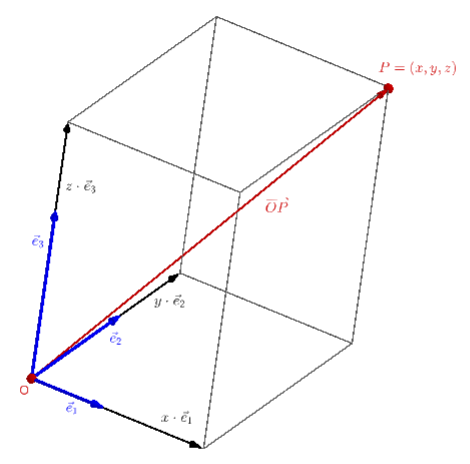
\includegraphics[width=0.7\textwidth]{cap_edolcv/dados/fig_edolcv_fg/fig}
  \caption{Esboço do gráfico da função gama $\Gamma(x)$.}
  \label{fig:edolcv_fg}
\end{figure}

\begin{obs} Vejamos as seguintes observações:
  \begin{enumerate}[a)]
  \item $\nexists\Gamma(0)$

    De fato, $\Gamma(0)$ não está definido pois
    \begin{equation}
      \lim_{x\to 0^-} \Gamma(x) = \lim_{x\to 0^-} \frac{\cancelto{\Gamma(1)=1}{\Gamma(x+1)}}{x} = -\infty
    \end{equation}
    e
    \begin{equation}
      \lim_{x\to 0^+} \Gamma(x) = \lim_{x\to 0^+} \frac{\cancelto{\Gamma(1)=1}{\Gamma(x+1)}}{x} = \infty
    \end{equation}

  \item $\nexists\Gamma(p)$, com $p$ inteiro negativo

    De fato, isto pode ser mostrado por indução a partir do item a) e da propriedade \eqref{eq:edolcv_fgp1}. Verifique!
  \end{enumerate}
\end{obs}

\begin{obs}
  Para números não naturais $x$, o valor de $\Gamma(x)$ só pode ser computado via técnicas de cálculo numérico. Uma das exceções, $\Gamma(\frac{1}{2})$, de fato
  \begin{align}
    \Gamma\left(\frac{1}{2}\right) &= \int_0^\infty z^{\frac{1}{2}-1}e^{-z}\,dz\\
    &= \int_0^\infty \frac{e^{-z}}{\sqrt{z}}\,dz
  \end{align}
  Fazendo a substituição $u=\sqrt{z}$, temos $\displaystyle du = \frac{dz}{2\sqrt{z}} = \frac{dz}{2u}$, obtemos
  \begin{align}
    \Gamma\left(\frac{1}{2}\right) &= \int_0^\infty \frac{e^{-u^2}}{u}\cdot 2u\,du \\
    &= 2\int_0^\infty e^{-u^2}\,du \\
    &= \int_{-\infty}^\infty e^{-u^2}\,du
  \end{align}
  Esta última é a conhecida integral de Gauss, a qual tem valor
  \begin{equation}
    \int_{-\infty}^\infty e^{-u^2}\,du = \sqrt{\pi}.
  \end{equation}
  Logo, concluímos que
  \begin{equation}\label{eq:edolcv_g12}
    {\color{blue}\Gamma\left(\frac{1}{2}\right) = \sqrt{\pi}}.
  \end{equation}
\end{obs}

\subsection{Função beta}

\begin{flushright}
  \href{https://archive.org/details/funcao-beta}{[Vídeo]} | [Áudio] | \href{https://phkonzen.github.io/notas/contato.html}{[Contatar]}
\end{flushright}

A \emph{função beta} (ou, integral de Euler de primeiro tipo) é definida por
\begin{equation}
  {\color{blue}B(x,y) = \int_0^1 z^{x-1}(1-z)^{y-1}\,dz},
\end{equation}
para quaisquer números reais positivos $x$ e $y$.

Sua relação com a função gama é dada por
\begin{equation}\label{eq:edolcv_bg}
  {\color{blue}B(x,y) = \frac{\Gamma(x)\Gamma(y)}{\Gamma(x+y)}}.
\end{equation}
De fato, temos
\begin{align}
  \Gamma(x)\Gamma(y) &= \int_0^\infty u^{x-1}e^{-u}\,du\cdot\int_0^\infty v^{y-1}e^{-v}\,dv \\
  &= \int_{v=0}^\infty\int_{u=0}^\infty u^{x-1}v^{y-1}e^{-(u+v)}\,du\,dv
\end{align}
Fazendo a mudança de variáveis $u=zt$ e $v=z(1-t)$, temos a jacobiana
\begin{align}
  J(u,v) &=
  \begin{vmatrix}
    \frac{\p u}{\p z} & \frac{\p u}{\p t}\\
    \frac{\p v}{\p z} & \frac{\p v}{\p t}
  \end{vmatrix}\\
  &= \begin{vmatrix}
    t & z\\
    (1-t) & -z
  \end{vmatrix}\\
  &= -z.
\end{align}
Logo,
\begin{align}
  \Gamma(x)\Gamma(y) &= \int_{z=0}^\infty\int_{t=0}^1 (zt)^{x-1}[z(1-t)]^{y-1}e^{-[zt+z(1-t)]}\,|J(u,v)|\,dt\,dz\\
  &= \int_{z=0}^\infty z^{x+y-1}e^{-z}\,dz\cdot \int_{t=0}^1 t^{x-1}(1-t)^{y-1}\,dt\\
  &= \Gamma(x+y) B(x,y),
\end{align}
o que nos fornece \eqref{eq:edolcv_bg}.

\begin{ex}
  \begin{equation}
    B\left(\frac{1}{2}, \frac{1}{2}\right) = \pi.
  \end{equation}
  De fato, de \eqref{eq:edolcv_bg}, temos
  \begin{align}
    B\left(\frac{1}{2}, \frac{1}{2}\right) &= \frac{\Gamma\left(\frac{1}{2}\right)\Gamma\left(\frac{1}{2}\right)}{\Gamma\left(\frac{1}{2}+\frac{1}{2}\right)}\\
    &= \frac{\sqrt{\pi}\sqrt{\pi}}{\Gamma(1)}\\
    &= \pi.
  \end{align}
\end{ex}

Para $n$ e $m$ números naturais não nulos, a propriedade \eqref{eq:edolcv_bg} mostra que a função beta guarda a seguinte relação com os coeficientes binomiais
\begin{equation}\label{eq:edolcv_fgcb}
  {\color{blue}B(n,m) = \frac{n+m}{nm}\cdot \frac{1}{\binom{n+m}{n}}},
\end{equation}
onde no denominador do último termo temos o coeficiente binomial
\begin{equation}
  \binom{n+m}{n} = \frac{(n+m)!}{n!(n+m-n)!} = \frac{(n+m)!}{n!m!}.
\end{equation}
De fato, \eqref{eq:edolcv_fgcb} decorre de \eqref{eq:edolcv_bg}, pois
\begin{align}
  B(n,m) &= \frac{\Gamma(n)\Gamma(m)}{\Gamma(n+m)} \\
  &= \frac{(n-1)!(m-1)!}{(n+m-1)!}\\
  &= \frac{n!m!}{(n+m)!}\frac{n+m}{nm}\\
  &= \frac{n+m}{nm}\cdot\frac{1}{\frac{(n+m)!}{n!m!}}\\
  &= \frac{n+m}{nm}\cdot \frac{1}{\binom{n+m}{n}}.
\end{align}

\subsection*{Exercícios resolvidos}

\begin{flushright}
  [Vídeo] | [Áudio] | \href{https://phkonzen.github.io/notas/contato.html}{[Contatar]}
\end{flushright}

\begin{exeresol}
  Calcule $\displaystyle\Gamma\left(\frac{3}{2}\right)$.
\end{exeresol}
\begin{resol}
  Da propriedade \eqref{eq:edolcv_fgp1} e de \eqref{eq:edolcv_g12} , temos
  \begin{align}
    \Gamma\left(\frac{3}{2}\right) &= \Gamma\left(\frac{1}{2}+1\right)\\
    &= \frac{1}{2}\Gamma\left(\frac{1}{2}\right)\\
    &= \frac{1}{2}\sqrt{\pi}.
  \end{align}
\end{resol}

\begin{exeresol}
  Verifique que
  \begin{equation}
    n! = \int_0^1 (-\ln s)^n\,ds.
  \end{equation}
\end{exeresol}
\begin{resol}
  Fazemos as mudanças de variáveis $t = -\ln s$, donde
  \begin{gather}
    dt = -\frac{1}{s}\,ds \\
    \Rightarrow ds = -e^{-t}\,dt
  \end{gather}
  Logo, temos
  \begin{align}
    \int_0^1 (-\ln s)^n\,ds &= -\int_\infty^0 t^ne^{-t}\,dt\\
    &= \int_0^\infty t^ne^{-t}\,dt\\
    &= \Gamma(n+1) \\
    &= n!
  \end{align}
\end{resol}

\begin{exeresol}
  Calcule $B(2,3)$.
\end{exeresol}
\begin{resol}
  Da propriedade \eqref{eq:edolcv_bg}, temos
  \begin{align}
    B(2,3) &= \frac{\Gamma(2)\Gamma(3)}{\Gamma(2+3)}\\
    &= \frac{1!\cdot 2!}{4!} \\
    &= \frac{2}{24} \\
    &= \frac{1}{12}.
  \end{align}
\end{resol}

\subsection*{Exercícios}

\begin{flushright}
  [Vídeo] | [Áudio] | \href{https://phkonzen.github.io/notas/contato.html}{[Contatar]}
\end{flushright}

\begin{exer}
  Calcule
  \begin{enumerate}[a)]
  \item $\Gamma(1)$\\
  \item $\Gamma(3)$\\
  \item $\Gamma(5)$\\
  \item $\Gamma(7)$
  \end{enumerate}
\end{exer}
\begin{resp}
  a)~1; b)~2; c)~24; d)~720
\end{resp}

\begin{exer}
  Calcule
  \begin{enumerate}[a)]
  \item $\Gamma\left(\frac{3}{2}\right)$\\
  \item $\Gamma\left(\frac{5}{2}\right)$\\
  \item $\Gamma\left(\frac{7}{2}\right)$\\
  \end{enumerate}
\end{exer}
\begin{resp}
  a)~$\frac{\sqrt{\pi}}{2}$; b)~$\frac{3\sqrt{\pi}}{4}$; c)~$\frac{15\sqrt{\pi}}{8}$
\end{resp}

\begin{exer}
  Calcule
  \begin{enumerate}[a)]
  \item $\Gamma\left(-\frac{1}{2}\right)$\\
  \item $\Gamma\left(-\frac{3}{2}\right)$
  \end{enumerate}
\end{exer}
\begin{resp}
  a)~$-2\sqrt{\pi}$; b)~$\frac{4\sqrt{\pi}}{3}$
\end{resp}

\begin{exer}
  Calcule
  \begin{enumerate}[a)]
  \item $B(1,1)$\\
  \item $B(2,2)$\\
  \item $B(3,2)$\\
  \end{enumerate}
\end{exer}
\begin{resp}
  a)~1; b)~$\frac{1}{6}$; c)~$\frac{1}{12}$;
\end{resp}

\begin{exer}
  Calcule
  \begin{enumerate}[a)]
  \item $B\left(\frac{1}{2},\frac{1}{2}\right)$\\
  \item $B\left(1,\frac{1}{2}\right)$\\
  \item $B\left(\frac{1}{2},\frac{3}{2}\right)$\\
  \end{enumerate}
\end{exer}
\begin{resp}
  a)~$\pi$; b)~2; c)~$\frac{\pi}{2}$
\end{resp}

\begin{exer}
  Verifique que
  \begin{equation}
    B(1,x) = \frac{1}{x},
  \end{equation}
  para todo $x$ número real positivo.
\end{exer}
\begin{resp}
  Dica: use \eqref{eq:edolcv_bg}.
\end{resp}

\section{Equação de Bessel}\label{cap_edolcv_sec_fbessel}

\begin{flushright}
  \href{https://archive.org/details/edo-bessel}{[Vídeo]} | [Áudio] | \href{https://phkonzen.github.io/notas/contato.html}{[Contatar]}
\end{flushright}

As funções de Bessel estão relacionadas as soluções das chamadas equações de Bessel
\begin{equation}\label{eq:bessel}
  x^2y'' + xy' + (x^2-\nu^2)y = 0,
\end{equation}
onde $y:x\mapsto y(x)$. Esta equação admite uma solução da forma
\begin{equation}\label{eq:bessel-s1}
  y(x) = \sum_{n=0}^\infty c_nx^{n+r},
\end{equation}
com $r$, $c_0\neq 0$ e $c_n$, $n=1,2,\ldots$ devem ser determinados. Para tanto, vamos substituir \eqref{eq:bessel-s1} em \eqref{eq:bessel}. Antes, observamos que
\begin{equation}
  y'(x) = \sum_{n=0}^\infty c_n(n+r)x^{n+r-1}
\end{equation}
e
\begin{equation}
  y''(x) = \sum_{n=0}^\infty c_n(n+r)(n+r-1)x^{n+r-2}
\end{equation}
Substituindo em \eqref{eq:bessel}, obtemos
\begin{gather}
  0 = x^2y'' + xy' + (x^2-\nu^2)y \\
  = \sum_{n=0}^\infty c_n(n+r)(n+r-1)x^{n+r} + \sum_{n=0}^\infty c_n(n+r)x^{n+r} \\
  + \sum_{n=0}^\infty c_nx^{n+r+2}- \nu^2\sum_{n=0}^\infty c_nx^{n+r}\\
  = c_0(r^2-r+r-\nu^2)x^r \\                              + x^r\sum_{n=1}^\infty c_n\left[(n+r)(n+r-1)+(n+r)-\nu^2\right]x^n+ x^r\sum_{n=0}^\infty c_nx^{n+2}\\
  = c_0(r^2-\nu^2)x^r + x^r\sum_{n=1}^\infty c_n\left[(n+r)^2-\nu^2\right]x^n \\
  + x^r\sum_{n=0}^\infty c_nx^{n+2}\label{eq:bessel-s2}
\end{gather}
Do primeiro termo, obtemos a chamada \emph{equação indicial}
\begin{equation}
  r^2 - \nu^2 = 0
\end{equation}
donde
\begin{equation}
  r_1 = \nu,\qquad r_2=-\nu.
\end{equation}
Ou seja, somente podemos esperar encontrar soluções para \eqref{eq:bessel} da forma \eqref{eq:bessel-s1} para estes valores de $r$.

Substituindo $r=r_1=\nu$ em \eqref{eq:bessel-s2}, obtemos
\begin{gather}
  0 = x^\nu\sum_{n=1}^\infty c_n\left[(n+\nu)^2-\nu^2\right]x^n + x^\nu\sum_{n=0}^\infty c_nx^{n+2}\\
  =  x^\nu\sum_{n=1}^\infty c_nn(n+2\nu)x^n + x^\nu\sum_{n=0}^\infty c_nx^{n+2}\\
  = x^\nu\left[c_1(1+2\nu)x + \underbrace{\sum_{n=2}^\infty c_nn(n+2\nu)x^n}_{m=n-2} + \underbrace{x^\nu\sum_{n=0}^\infty c_nx^{n+2}}_{m=n}\right]\\
  = x^\nu\left[c_1(1+2\nu)x \right.\\
    \left. + \sum_{m=0}^\infty c_{m+2}(m+2)(m+2+2\nu)x^{m+2} + x^\nu\sum_{m=0}^\infty c_mx^{m+2}\right]\\
  = x^\nu\left\{c_1(1+2\nu)x + \sum_{m=0}^\infty \left[c_{m+2}(m+2)(m+2+2\nu) + c_m\right]x^{m+2}\right\}
\end{gather}
Logo,
\begin{equation}
  c_1(1+2\nu) = 0
\end{equation}
e, para $m=0,1,2,\infty$,
\begin{equation}
  (m+2)(m+2+2\nu)c_{m+2}+c_m = 0
\end{equation}
ou, equivalentemente,
\begin{equation}
  c_{m+2} = \frac{-c_m}{(m+2)(m+2+2\nu)}
\end{equation}

Escolhendo $c_1=0$, temos
\begin{equation}
  c_3=c_5=c_7=\cdots=0.
\end{equation}
Agora, para $m+2=2n$, $n=1,2,3,\ldots$, temos
\begin{equation}
  c_{2n} = -\frac{c_{2n-2}}{2^2n(n+\nu)}.
\end{equation}
Daí, segue que
\begin{align}
  c_2 &= -\frac{c_0}{2^2\cdot 1\cdot (1+\nu)}\\
  c_4 &= -\frac{c_2}{2^2\cdot 2\cdot (2+\nu)}\\
  &= \frac{c_0}{2^4\cdot 2!\cdot (1+\nu)(2+\nu)}\\
  c_6 &= -\frac{c_4}{2^2\cdot 3\cdot (3+\nu)}\\
  &= -\frac{c_0}{2^6\cdot 3!\cdot (1+\nu)(2+\nu)(3+\nu)}\\
  &\vdots\\
  c_{2n} &= \frac{(-1)^nc_0}{2^{2n}n!(1+\nu)(2+\nu)\cdots(n+\nu)}
\end{align}
Da propriedade da função gama
\begin{equation}
  \Gamma(x+1) = x\Gamma(x)
\end{equation}
temos que
\begin{align}
  \Gamma(1+\nu+1) &= (1+\nu)\Gamma(1+\nu)\\
  \Gamma(1+\nu+2) &= (2+\nu)\Gamma(2+\nu)=(1+\nu)(2+\nu)\Gamma(1+\nu)\\
  &\vdots\\
  \Gamma(1+\nu+n) &= (1+\nu)(2+\nu)\cdots(n+\nu)\Gamma(1+\nu). 
\end{align}
Com isso, escolhendo
\begin{equation}
  c_0 = \frac{1}{2^\nu\Gamma(1+\nu)}
\end{equation}
concluímos que
\begin{equation}
  c_{2n} = \frac{(-1)^n}{2^{2n+\nu}n!\Gamma(1+\nu+n)}
\end{equation}
e
\begin{equation}
  c_{2n-1}=0
\end{equation}
para $n=1,2,3,\ldots$.

Com tudo isso, obtivemos a seguinte solução para a equação de Bessel
\begin{equation}
  y(x) = \sum_{n=0}^\infty \frac{(-1)^n}{2^{2n+\nu}n!\Gamma(1+\nu+n)}x^{2n+\nu}
\end{equation}
ou, equivalentemente,
\begin{equation}
  y(x) = \sum_{n=0}^\infty \frac{(-1)^n}{n!\Gamma(1+\nu+n)}\left(\frac{x}{2}\right)^{2n+\nu}.
\end{equation}
Esta é conhecida como \emph{função de Bessel de primeira espécie} de ordem $\nu$ e é usualmente denotada por
\begin{equation}\label{eq:bessel-1esp-nu}
  {\color{blue}J_\nu(x) = \sum_{n=0}^\infty \frac{(-1)^n}{n!\Gamma(1+\nu+n)}\left(\frac{x}{2}\right)^{2n+\nu}}. 
\end{equation}
Pode-se mostrar que se $\nu\geq 0$, a série converge para $x\in [0, \infty)$.

  Outra solução da equação de Bessel é obtida tomando $r=r_2=-\nu$. Procedendo de forma análoga, obtemos a solução
  \begin{align}
    y(x) &= J_{-\nu}(x)\\
    &= \sum_{n=0}^\infty \frac{(-1)^n}{n!\Gamma(1-\nu+n)}\left(\frac{x}{2}\right)^{2n-\nu},
  \end{align}
  a qual é chamada de função de Bessel de primeira espécie de ordem $-\nu$.

  Agora, vamos discutir sobre a \emph{solução geral} da equação de Bessel. Pode-se mostrar \emph{se $\nu$ não é um número inteiro, então $J_\nu(x)$ e $J_{-\nu}(x)$ são soluções linearmente independentes}. Logo, temos a solução geral
  \begin{equation}
    y(x) = c_1J_\nu(x) + c_2J_{-\nu}(x),\quad \nu\not\in\mathbb{Z}.
  \end{equation}

  \begin{ex}
    A solução geral da equação de Bessel de ordem $\nu=1/3$
    \begin{equation}
      x^2y'' + xy' + \left(x^2 - \frac{1}{9}\right)y = 0
    \end{equation}
    é
    \begin{equation}
      y(x) = c_1J_{\frac{1}{3}}(x) + c_2J_{-\frac{1}{3}}(x).
    \end{equation}
  \end{ex}

  \subsection{Função de Bessel de segunda espécie}

  \begin{flushright}
    [Vídeo] | [Áudio] | \href{https://phkonzen.github.io/notas/contato.html}{[Contatar]}
  \end{flushright}
  
  A \emph{função de Bessel de segunda espécie} de ordem $\nu$ é dada por
  \begin{equation}
    Y_\nu(x) = \frac{J_\nu(x)\cos(\nu\pi)-J_{-\nu}(x)}{\sen(\nu\pi)}
  \end{equation}
  Para $\nu$ não inteiro, $Y_\nu(x)$ e $J_\nu(x)$ são soluções linearmente independentes da equação de Bessel. Agora, pode-se mostrar que quando $\nu\to m$ número inteiro, o seguinte limite está bem definido
  \begin{equation}
    Y_m(x) = \lim_{\nu\to m} Y_\nu(x).
  \end{equation}
  Além disso, para $m$ número inteiro, $Y_m(x)$ e $J_m(x)$ são linearmente independentes. Logo, a \emph{solução geral} da equação de Bessel de ordem $m$ é
  \begin{equation}
    {\color{blue}y(x) = c_1J_m(x) + c_2Y_m(x)},
  \end{equation}
  onde $Y_\nu(x)$ é chamada de \emph{função de Bessel de segunda espécie} de ordem $\nu$.

  \begin{ex}
    A solução geral da equação de Bessel de ordem $\nu=3$
    \begin{equation}
      x^2y'' + xy' + \left(x^2 - 9\right)y = 0
    \end{equation}
    é
    \begin{equation}
      y(x) = c_1J_{3}(x) + c_2Y_3(x).
    \end{equation}  
  \end{ex}

  \subsection*{Exercícios resolvidos}

    \begin{flushright}
    [Vídeo] | [Áudio] | \href{https://phkonzen.github.io/notas/contato.html}{[Contatar]}
  \end{flushright}

  \begin{exeresol}
    Forneça a solução geral da equação
    \begin{equation}
      x^2y'' + xy' + x^2y = 0
    \end{equation}
  \end{exeresol}
  \begin{resol}
    Esta é a equação de Bessel de ordem $\nu = 0$. A solução geral é combinação linear da função de Bessel de primeira espécie $J_0(x)$ com a função de Bessel de segunda espécie $Y_0(x)$, i.e.
    \begin{equation}
      y(x) = c_1J_0(x) + c_2Y_0(x).
    \end{equation}
  \end{resol}


  \begin{exeresol}
    Verifique se
    \begin{equation}
      J_{\frac{1}{2}}(x) = \left(\frac{2}{\pi x}\right)^{\frac{1}{2}}\sen x,\quad x>0.
    \end{equation}
    Dica:
    \begin{equation}\label{eq:bessel-dica-1}
      \Gamma\left(\frac{1}{2}+n\right) = \frac{(2n)!}{4^nn!}\sqrt{\pi}.
    \end{equation}
  \end{exeresol}
  \begin{resol}
    Da definição da função de Bessel de primeira espécie de ordem $\nu$ \eqref{eq:bessel-1esp-nu}, temos
    \begin{equation}
      J_{\frac{1}{2}}(x) = \sum_{n=0}^\infty \frac{(-1)^n}{n!\Gamma\left(1+\frac{1}{2}+n\right)}\left(\frac{x}{2}\right)^{2n+\frac{1}{2}}.
    \end{equation}
    Usando \eqref{eq:bessel-dica-1}, temos
    \begin{align}
      \Gamma\left(1+\frac{1}{2}+n\right) &= \frac{[2(n+1)]!}{4^{n+1}(n+1)!}\sqrt{\pi}\\
      &= \frac{[2(n+1)]!}{2^{2n+2}(n+1)!}\sqrt{\pi}. 
    \end{align}
    Substituindo na função de Bessel, obtemos
    \begin{align}
      J_{\frac{1}{2}}(x) &= \sum_{n=0}^\infty \frac{(-1)^n}{n!\frac{[2(n+1)]!}{2^{2n+2}(n+1)!}\sqrt{\pi}}\left(\frac{x}{2}\right)^{2n+\frac{1}{2}}\\
      &= \left(\frac{x}{2}\right)^{\frac{1}{2}}\frac{1}{\sqrt{\pi}}\sum_{n=0}^\infty \frac{(-1)^n2^{2n+2}(n+1)!}{n![2(n+1)]!2^{2n}}x^{2n}\\
      &= \left(\frac{x}{2\pi}\right)^{\frac{1}{2}}\sum_{n=0}^\infty \frac{(-1)^n2^2(n+1)}{[2(n+1)]!}x^{2n}\\
      &= \left(\frac{x}{2\pi}\right)^{\frac{1}{2}}2\sum_{n=0}^\infty \frac{(-1)^n(2n+2)}{(2n+2)(2n+1)!}x^{2n}\\
      &= \frac{2\sqrt{x}}{x\sqrt{2}\sqrt{\pi}}\sum_{n=0}^\infty \frac{(-1)^n}{(2n+1)!}x^{2n+1}\\
      &= \sqrt{\frac{2}{\pi x}}\sen x,
    \end{align}
    lembrando que a expansão em série de MacLaurin
    \begin{equation}
      \sen x = \sum_{n=0}^\infty \frac{(-1)^n}{(2n+1)!}x^{2n+1}.
    \end{equation}
  \end{resol}

  \subsection*{Exercícios}

    \begin{flushright}
    [Vídeo] | [Áudio] | \href{https://phkonzen.github.io/notas/contato.html}{[Contatar]}
  \end{flushright}

  \begin{exer}
    Forneça a solução da equação de Bessel
    \begin{equation}
      x^2y'' + xy' + (x^2-\frac{1}{16})y = 0.
    \end{equation}
  \end{exer}
  \begin{resp}
    $y(x) = c_1J_{\frac{1}{4}}(x) + c_2J_{-\frac{1}{4}}(x)$
  \end{resp}


  \begin{exer}
    Forneça a solução da equação de Bessel de ordem um
    \begin{equation}
      x^2y'' + xy' + (x^2-1)y = 0.
    \end{equation}
  \end{exer}
  \begin{resp}
    $y(x) = c_1J_1(x) + c_2Y_1(x)$
  \end{resp}

  \begin{exer}
    Forneça a solução da equação
    \begin{equation}
      4x^2(y''+y) + 4xy' -9y = 0.
    \end{equation}
  \end{exer}
  \begin{resp}
    $y(x) = c_1J_{\frac{3}{2}}(x) + c_2J_{-\frac{3}{2}}(x)$
  \end{resp}

  \begin{exer}
    Calcule $J_0'(x)$ para $x>0$\footnote{Pode-se mostrar que $J_0$ é uma função analítica em $x=0$. Veja, por exemplo, \cite[Capítulo 5., Seção 5.7.]{Boyce2020}}.
  \end{exer}
  \begin{resp}
    $J_0'(x)=-J_1(x)$
  \end{resp}

  \begin{exer}
    Verifique se
    \begin{equation}
      J_{-\frac{1}{2}}(x) = \left(\frac{2}{\pi x}\right)^{\frac{1}{2}}\cos x,\quad x>0.
    \end{equation}
  \end{exer}
  \begin{resp}
    Dicas:
    \begin{equation}
      \Gamma\left(\frac{1}{2}+n\right) = \frac{(2n)!}{4^nn!}\sqrt{\pi}.
    \end{equation}
    \begin{equation}
      \cos x = \sum_{n=0}^\infty \frac{(-1)^n}{(2n)!}x^{2n}.
    \end{equation}  
  \end{resp}

  \begin{exer}
    Calcule a solução geral da equação de Bessel de ordem um meio
    \begin{equation}
      x^2y'' + xy' + \left(x^2-\frac{1}{4}\right)y = 0.
    \end{equation}
  \end{exer}
  \begin{resp}
    $y(x) = c_1\frac{\sen x}{x^{1/2}} + c_2\frac{\cos x}{x^{1/2}}$
  \end{resp}


%resposta dos exercícios
\ifisbook


\chapter*{Resposta dos Exercícios}\label{cap_respostas}
\addcontentsline{toc}{chapter}{Respostas dos Exercícios}

\shipoutAnswer
\fi

% endnotes
\clearpage
\phantomsection
\addcontentsline{toc}{chapter}{Notas}
\theendnotes


%%references
\ifisbook
\clearpage
\phantomsection
\renewcommand\bibname{Referências}
\addcontentsline{toc}{chapter}{\bibname}
\fi

\begin{thebibliography}{99}
  
  \bibitem{Boyce2017a}
    Boyce, W.E. \& DiPrima, R.C., Equações diferenciais elementares e problemas de valores de contorno, 11. ed., LTC, 2020. \texttt{ISBN: 978-1-119-38164-8}
    
  \bibitem{Cengel2014}
    Çengel, Y. A., Equações diferenciais, 1. ed., AMGH, 2014. \texttt{ISBN: 9788580553482}

  \bibitem{Oliveira2003}
    Oliveira, E. C. \& Maiorino, J. E., Introdução aos métodos de matemática aplicada, 2. ed., Unicamp, 2013. \texttt{ISBN: 8526806386}

  \bibitem{Zill2016}
  Zill, D. G., Equações diferenciais com aplicações em modelagem, 10. ed., Cengage Learning, 2016. \texttt{ISBN: 978-85-221-2402-2}
\end{thebibliography}

% índice remissivo
\ifisbook
\printindex
\fi

\end{document}
